\chapter{Syntaktische Markierungen}\label{syntax}

Auf der syntaktischen Ebene manipuliert das \hai{{\LiJi}} besonders stark im Bereich der Verbsyntax (Abschnitte \ref{verbsyntax}, \ref{overraising}, \ref{noipp}, \ref{kommenzugehen}) und mittels der Suggestion veränderter Grundwortstellung über Extrapositionen (Abschnitt \ref{VOOV}). Kleinere Manipulationen betreffen die \isi{Negationskongruenz} (Abschnitt \ref{negation}) und die Relativsatzeinleitung (Sektion \ref{relativpartikel}). 

Es ist besonders auffällig, dass wir im \hai{{\LiJi}} viele syntaktische Manipulationsstrategien vorfinden, die direkt in die Grundwortstellung eingreifen (Abschnitte \ref{verbsyntax} u. \ref{VOOV}). Damit stellt uns die Beschreibung der syntaktischen Manipulationen im Gegensatz zur Phonologie und \isi{Morphologie} vor das Problem, dass es sich nur schwer bestimmen lässt, wo die Matrixsprache endet und wo die Zielsprache beginnt. Die \mbox{Definition} eines syntaktischen Phänomens hängt stark davon ab, welche Grundwortstellung vorausgesetzt wird. Neuhochdeutsch wird in dieser Arbeit als eine Sprache mit \hai{{\OV}}-Grundwortstellung behandelt.\footnote{Deutsch ist sicher keine prototypische \hai{{\OV}}-Sprache wie z.\,B.\, Japanisch oder Türkisch, erfüllt jedoch die nötigen Grundvoraussetzungen (vgl.\, \citealt{Vikner2001}, \citealt{Haider2010b}). Besonders der Blick auf die Sprachgeschichte der deutschen Grundwortstellung verdeutlicht, wie flexibel und v.\,a.\, wie jung das deutsche System ist (vgl.\, \citealt{Schallert2010}, \citealt{Haider2010}).} Für das moderne Ostjiddische hingegen wird ein \hai{{\OV}}/\hai{{\VO}}-Mischsystem angenommen, dass erst ab der Schriftsprache des 19. Jahrhunderts systematisch verwendet wird (vgl.\, \citealt{Santorini1989,Santorini1992,Santorini1993b,Santorini1993a,Santorini1994,Santorini1995};\,\citealt[203–207]{Krogh2007};\,\citealt[97–134]{Haider2013}). Für das Westjiddische im 19. und 20. Jahrhundert, wie auch für ältere Sprachstufen des Jiddischen, wird eine Grundwortstellung parallel zum Deutschen angenommen, die eine deutlichere Ausrichtung an Grundmustern von \hai{{\OV}}-Sprachen zeigt als es im modernen Jiddisch der Fall ist (vgl.\, \citealt{Santorini1989, Santorini1992, Santorini1993a, Santorini1993b, Santorini1994, Santorini1995}). Da die neuhochdeutsche Literatursprache die Matrixsprache zum \hai{{\LiJi}} darstellt, wird die \hai{{\OV}}-Grundwortstellung als dessen Matrixstruktur gesetzt. Emulationen von \hai{{\VO}}-Eigenschaften des modernen Jiddischen werden als Manipulationen an der \hai{{\OV}}-Ausgangssituation analysiert. Das Prinzip der emulierenden \isi{Imitation} wird im Bereich der \isi{Syntax} besonders deutlich: Ein Sprecher einer \hai{{\OV}}-Sprache kann die Wortstellung dieser Sprache nur im Rahmen seines muttersprachlichen Systems manipulieren. Die Fähigkeit, zwischen zwei Systemen zu \textit{switchen}, ist auf bilinguale Sprecher beschränkt. Wie beim Zweitspracherwerb werden bei der sprachlichen \isi{Emulation} Regeln im Kontrast zur Muttersprache (Matrixsprache) formuliert und angewendet. Alle erhobenen und im Folgenden analysierten syntaktischen Phänomene des \hai{{\LiJi}} werden auf Basis der Grundmuster der neuhochdeutschen Schriftsprache definiert. Es besteht darin zu den vorhergegangenen Analysen keinerlei Unterschied. Da dieses Vorgehen aber gerade im Bereich der \isi{Syntax} seine Tücken zeigt, scheint es ratsam, dieses Prinzip erneut zu formulieren und den syntaktischen Einzelanalysen vorwegzuschicken.  

Aus dem Umstand heraus, dass die einschlägigen Arbeiten zur jiddischen \isi{Syntax} der theoretischen Linguistik (insbes. der generativen Linguistik) entstammen, werden die in der Literatur üblichen Konzepte verwendet und auf die Daten des \hai{{\LiJi}} angewandt, da nur so ein wissenschaftlicher Diskurs möglich ist. 


  \section{Abfolgevariation im Verbalkomplex}\label{verbsyntax}
%  %\noindent
Diese Arbeit folgt den von \citet{Bech1955,Bech1957} formulierten Prinzipien und Notationen zum deutschen Verbgefüge. In einer Verbkette regiert jedes Verb den Status seines infiniten Komplements. Entscheidend für die Analyse verbaler Cluster sind die drei verschiedenen Status, die \citet{Bech1955,Bech1957} für die Rektion ansetzt: Ein Verb regiert den Status seines infiniten Komplements. Von Verben im 1. Status wird der reine \isi{Infinitiv} gefordert, während das Infinitum des 2. Status im \textit{zu}-\isi{Infinitiv} steht und im 3. Status im Perfektpartizip:
  \begin{center}
   $ V1 \xrightarrow{regiert} V2 \xrightarrow{regiert} V3  $ \\
     \end{center}
  Entscheidend daran ist, dass der Status immer nur vom unmittelbar nächsten regierenden verbalen Element zugewiesen wird. Dabei verhält es sich so, dass bestimmte Verbklassen gewisse Status bevorzugen und damit die \isi{Statusrektion} sehr streng organisiert ist. So fordern Modalverben den 1. Status ihres Komplements (\ref{1ST}), Vollverben hingegen immer den 2. Status (\ref{2ST}) und (tempusbildende) Auxiliare dementsprechend den 3. Status (\ref{3ST}). Daraus ergibt sich für das Verbgefüge der rechten Satzklammer in (\ref{4ST}) die Notation entsprechend der Abhängigkeiten \hai{V\textsubscript{3}}–\hai{V\textsubscript{2}}–\hai{V\textsubscript{1}}. 
 
 
  
  
      \eenumsentence{

      \item \textit{weil sie denken}\textsubscript{1. Status} \textit{muss}\label{1ST}
      \item \textit{weil sie zu denken}\textsubscript{2. Status} \textit{versucht}\label{2ST}
           \item \textit{weil sie gedacht}\textsubscript{3. Status} \textit{hat}\label{3ST}     
                  \item  \textit{weil sie gedacht}\textsubscript{3} \textit{haben}\textsubscript{2}  \textit{soll}\textsubscript{1}\label{4ST}   


      }
  
 \label{Verbabfolgedeutsch} Im Schriftdeutschen als \hai{{\OV}}-Sprache erfolgt die Serialisierung zweigliedriger Verbketten innerhalb der rechten Satzklammer (\hai{{\RSK}}) immer nach dem Muster \hai{V}\textsubscript{2}–\hai{V}\textsubscript{1} (\ref{dreiverben_dt});\, \,%rs s. Bsp. 
 d.\,h.\, die \hai{VP} ist hier kopf-initial (Abbildung \ref{kopfxbar}a).\, Andere \hai{{\OV}}-Spra\-chen wie Niederländisch (s.\, Bsp.\,  \ref{dreiverben_ndl}) \,%rs s. Bsp. 
 oder diverse deutsche Varietäten (vgl.\, \citealt[75]{Vikner2001})  können von dieser Abfolgeregel abweichen. Diese Flexibilität innerhalb der \hai{VP} ist eine Besonderheit von \hai{{\OV}}-Sprachen. Die Grundabfolge in \hai{{\VO}}-Sprachen (wie etwa dem Englischen oder Französischen) ist immer kopf-final \hai{V}\textsubscript{1}–\hai{V}\textsubscript{2}, s. Bsp. (\ref{dreiverben_engl}), (\ref{dreiverben_fr});\, Abbildung \ref{kopfxbar}b. Generell lässt sich festhalten, dass \hai{{\VO}}-Sprachen keinerlei Abfolgevarianz bei zusammengesetzten Verbformen aufweisen, während dies bei \hai{{\OV}}-Sprachen durchaus der Fall sein kann (siehe z.B. Niederländisch oder Deutsch).

 \begin{figure}[htbp]
 \begin{center}
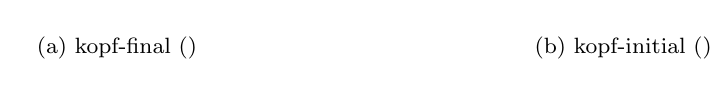
\begin{tikzpicture}
\node [below = 5.8em] (a) {\footnotesize{(a) kopf-final (\hai{{\OV}})}};
\Tree [.VP [.$\triangle$ ] 
             [.\textsc{V'} [.\textsc{XP} ] [.V° ]]
        ]
\begin{scope}[xshift=6cm]
 \node [below = 5.8em] (b) {\footnotesize{(b) kopf-initial (\hai{{\VO}})}};
\Tree  [.VP [.$\triangle$ ] 
             [.\textsc{V'} [.V° ] [.\textsc{XP} ]]
        ]
\end{scope}


\end{tikzpicture}\caption{Die \hai{VP} in \hai{{\OV}}- und \hai{{\VO}}-Sprachen 
%(vgl.\, \citealt[262, Abbildung 1]{Santorini1993a})
}\label{kopfxbar}
 \end{center}
 \end{figure}

 
 


 
 
  In \hai{{\VO}}-Sprachen gibt es keine Varianz in der Verbabfolge. Das moderne Jiddische, welches in dieser Arbeit den Argumenten Santorinis (\citeyear{Santorini1993b}) und Haiders (\citeyear{Haider2013}) folgend als gemischte \hai{{\OV}}/\hai{{\VO}}-Sprache typisiert wird, zeigt somit auch im Verbalkomplex Strukturen beider Grundwortstellungstypen (\ref{dreiverben_oj}). Allein damit, dass im Ostjiddischen Verbstellungsvariation vorliegt, ist eine \hai{{\VO}}-Grundwort-stellung für diese Sprache auszuschließen. Im Bereich der Verbserialisierung verhält sich \ili{Ostjiddisch} eher einer \hai{{\OV}}-Sprache entsprechend (vgl.\, \citealt[170–173]{Geilfuss1990}). 
 
  \eenumsentence{\label{dreiverben_dt} 
      \item dt. \textit{Ein Haus muss} \textit{gebaut}\textsubscript{2} werden\textsubscript{1}\\
     (zitiert n. Vikner 2001:\,75)\label{AbfolgeVerben_1}
    \item dt. *\textit{Ein Haus muss} \textit{werden}\textsubscript{1} \textit{gebaut}\textsubscript{2}\\
     (zitiert n. Vikner 2001:\,75)\label{AbfolgeVerben_2}
  }
  
  
      \eenumsentence{\label{dreiverben_ndl} 
   \item {\ndl} \textit{Een huis moet} \textit{gebouwd}\textsubscript{2} \textit{worden}\textsubscript{1}\\
     (zitiert n. Vikner 2001:\,75)\label{AbfolgeVerben_5}
  \item {\ndl} \textit{Een huis moet} \textit{worden}\textsubscript{1} \textit{gebouwd}\textsubscript{2}\\
     (zitiert n. Vikner 2001:\,75)\label{AbfolgeVerben_6}
}

       
   \eenumsentence{\label{dreiverben_oj} 
     \item {\oj} \textit{A hoyz muz} \textit{geboyt}\textsubscript{2} \textit{vern}\textsubscript{1}\\
     (zitiert n. Besten \& Moed-van Walraven 1986:\,117. Bsp. 16;\\ vgl.\, Vikner 2001:\,74)\label{AbfolgeVerben_7}
     
     \item {\oj} \textit{A hoyz muz} \textit{vern}\textsubscript{1} \textit{geboyt}\textsubscript{2}\\ 
     (zitiert n. Besten \& Moed-van Walraven 1986:\,117. Bsp. 16;\\ vgl.\, Vikner 2001:\,74)\label{AbfolgeVerben_8}

   }
  
     \eenumsentence{\label{dreiverben_engl} 
   \item {\engl} *\textit{A house must} \textit{built}\textsubscript{1} \textit{be}\textsubscript{2}\\
   (zitiert n. Besten \& Moed-van Walraven 1986:\,117. Bsp. 16;\\ vgl.\, Vikner 2001:\,74)\label{AbfolgeVerben_3}
   \item {\engl} \textit{A house must} \textit{be}\textsubscript{1} \textit{built}\textsubscript{2}\\
   (zitiert n. Besten \& Moed-van Walraven 1986:\,117. Bsp. 16;\\ vgl.\, Vikner 2001:\,74)\label{AbfolgeVerben_4}
} 
 
  \eenumsentence{\label{dreiverben_fr} 
     \item {\fr} *\textit{Une maison doit} \textit{construite}\textsubscript{2} \textit{être}\textsubscript{1}\label{AbfolgeVerben_11}
     
     \item {\fr} \textit{Une maison doit} \textit{être}\textsubscript{1} \textit{construite}\textsubscript{2}\\ 
   
     }

 
 Die ostjiddischen Abfolgemuster unterscheiden sich jedoch stark vom Westjiddischen. Zwar stehen noch detaillierte Analysen zur Verbsyntax des späten Westjiddischen aus, doch konnte Santorini (1989, 1992, 1993a, 1993b, 1994, insbes. 1995) zeigen, dass sich die kopf-initiale Verbstellung im Ostjiddischen bereits Ende des 16. Jahrhunderts gegenüber der kopf-finalen Verbstellung durchsetzen konnte, während im Westjiddischen zwischen dem  16. und 17. Jahrhundert noch beide Strukturen bis ins 18. Jahrhundert – für das 19. und 20. Jahrhundert hat Santorini keine Daten zum Westjiddischen – konkurrierten. Ihre Quellen zum Westjiddischen zeigen prinzipiell eine stärkere Ausrichtung am deutschen System als die ostjiddischen Quellen. Für das späte \ili{Westjiddisch} des 19. Jahrhunderts ist eher eine kopf-finale Grundstruktur anzunehmen als eine kopf-initiale.


 \hai{{\OV}}-Sprachen erlauben im Gegensatz zu \hai{{\VO}}-Sprachen mehr Wortstellungsvariation. Die Abweichung der Grundstellung der Verben innerhalb der \hai{{\RSK}} wird als \quein{verb raising} (\hai{{\VR}}) bezeichnet (vgl.\, \citealt{Evers1975};Abbildung \ref{baumVR}). In einer \hai{{\OV}}-Sprache wie dem Deutschen ist die übliche Abfolge bei zweigliedrigen Verbketten \hai{V}\textsubscript{2}–\hai{V}\textsubscript{1} (s. Abschnitt \,%rs Abschnitt
 \ref{Verbabfolgedeutsch}, S.\, \pageref{Verbabfolgedeutsch}). Unter \hai{{\VR}} fallen damit Belege des Musters \hai{V}\textsubscript{1}–\hai{V}\textsubscript{2}, wie in (\ref{BSPVR12}) illustriert. 


  \eenumsentence{\label{BSPVR}
    \item dt. \textit{Da habt ihr mir nicht folgen}\textsubscript{2} \textit{wollen}\textsubscript{1}\label{BSPVR21}  
       \item dt. \textit{Da habt ihr mir nicht wollen}\textsubscript{1} \textit{folgen}\textsubscript{2}\label{BSPVR12}
  }
  

\vspace{0.2cm}
 


\begin{figure}

\fittable{
\begin{tikzpicture}[sibling distance=36pt] 
 \Tree [.VP\textsubscript{1} [.VP\textsubscript{2} [.VP\textsubscript{3} [.\node(V3){\=V\textsubscript{3}};V\textsubscript{3} ] ] 
 [.\=V\textsubscript{2} \node(V1){V\textsubscript{2}};] ] 
[.\node(v1g){\=V\textsubscript{1}};V\textsubscript{1} ]
]
\draw[semithick,->] (V3) to[bend right=20] (V1);
%[.V\textsubscript{1} V\textsubscript{1} ]]

\begin{scope}[xshift=4cm,yshift=12pt]
 \tikzset{every tree node/.style={align=center, anchor=north}}
\Tree [.VR\\[14pt]{$\Rightarrow$} ]
\end{scope}

\begin{scope}[xshift=10cm]
 \Tree [.VP\textsubscript{1} [.\node(vp2g){VP\textsubscript{2}};[.VP\textsubscript{3} e ] [.\node(V2){\=V\textsubscript{2}}; [.V\textsubscript{2} [.V\textsubscript{2} ] [.\=V\textsubscript{3} V\textsubscript{3} ]
] ] ] 
[.\=V\textsubscript{1} \node(V1){V\textsubscript{1}};]
]
\draw[semithick,->] (V2) to[bend right=20] (V1);

\end{scope}

 \end{tikzpicture}
\caption{\hai{{\VR}} nach den Besten \& Edmondson 
 (\citeyear[196, Abbildung 76]{BestenEdmondson1983})}
\label{baumVR}	%Baum
}

 \end{figure}


 In älteren Sprachstufen des Jiddischen findet sich bereits \hai{{\VR}} belegt, wie in (\ref{IPPsantorinib}) ( \ref{IPPsantorini}) (S.\, \pageref{IPPsantorini})  zu sehen ist (vgl.\, \citealt{Santorini1989,Santorini1992,Santorini1993b,Santorini1993a,Santorini1994,Santorini1995}). \hai{{\VR}} ist auch vielfach für die Diachronie des Deutschen beschrieben und analysiert worden (vgl.\, \citealt{Maurer1926,Haerd1981,Ebert1980,Ebert1981,Ebert1998,Agel2001,Ramers2005,Axel2007,Sapp2006,Sapp2011}). Während das Schriftdeutsche im Verlauf des Frühneuhochdeutschen die relativ strikte Abfolge \hai{V}\textsubscript{2}–\hai{V}\textsubscript{1} durchsetzt,\footnote{Krasselt (\citeyear{Krasselt2013}) zeigt, dass selbst noch in der modernen Umgangssprache des Deutschen Variation und eine breite Akzeptabilität bei Zwei- und Dreiverbclustern besteht.} entwickelt sich das Jiddische komplementär und baut die \hai{V}\textsubscript{1}–\hai{V}\textsubscript{2} Serialisierung weiter aus. Im modernen Ostjiddischen ist damit die Grundstellung des Deutschen nicht gegeben;\, hier sind beide Abfolgevarianten möglich (\ref{BSPVRJI}) (vgl.\, \citealt{Santorini1989,Santorini1992,Santorini1993b,Santorini1993a,Santorini1994,Santorini1995,BestenWalraven1986}). 
  
  
   \eenumsentence{\label{BSPVRJI}
   
    \item {\mj} \textit{da habt ir mir nit veln}\textsubscript{1} \textit{falgn}\textsubscript{2} (\hai{DCY}:\,{\wj}\,Gerichtsprotokolle von 1465)\\
   \sem{da habt ihr mir nicht folgen wollen (wörtl. wollen folgen)}\label{IPPsantorinib}

    \item {\oj} {\RL{ד{א\makebox(-1.25,-1.25)[r]{\libertineGlyph{uni05B8}}} ה{א\makebox(-1.25,-1.25)[r]{\libertineGlyph{uni05B8}}}בט איר מיר ניט געוו{א\makebox(-1.25,-1.25)[r]{\libertineGlyph{uni05B8}}}לט {פ\makebox(-0.8,9)[r]{\libertineGlyph{uni207B}}}{א\makebox(-1.25,-1.25)[r]{\libertineGlyph{uni05B8}}}לגן}} \textit{do hobt ir mir nit gevolt}\textsubscript{2} \textit{folgn}\textsubscript{1}\\
     \sem{da habt ihr mir nicht folgen wollen (wörtl. gewollt folgen)} \label{BSPVRji21}  
       \item {\oj} {\RL{ד{א\makebox(-1.25,-1.25)[r]{\libertineGlyph{uni05B8}}} ה{א\makebox(-1.25,-1.25)[r]{\libertineGlyph{uni05B8}}}בט איר מיר ניט {פ\makebox(-0.8,9)[r]{\libertineGlyph{uni207B}}}{א\makebox(-1.25,-1.25)[r]{\libertineGlyph{uni05B8}}}לגן געוו{א\makebox(-1.25,-1.25)[r]{\libertineGlyph{uni05B8}}}לט}} \textit{do hobt ir mir nit folgn}\textsubscript{1} \textit{gevolt}\textsubscript{2}\\ 
       \sem{da habt ihr mir nicht folgen wollen (wörtl. folgen gewollt)}\label{BSPVRji12}   
       
                }
  
  
Die deutschen Dialekte (und auch andere westgermanische Varietäten) zeigen eine deutlich höhere Variabilität innerhalb der \hai{VP}, als es die moderne Schriftsprache vermuten lässt (u.\,a.\, \citealt{Loetscher1978,BestenEdmondson1983,Patocka1997,Vikner1995,Vikner2001,Seiler2004,Wurmbrand2004,Wurmbrand2006,Wurmbrand2012,Sapp2006,Sapp2011,DubenionSmith2010,Schallert2014}). Die Möglichkeit, dass \hai{{\VR}}-Belege des \hai{chrLiJi1} auf deutsch-dialektalen Formen fußen, ist damit nicht auszuschließen. Doch auch in Quellen des späten Westjiddischen finden sich beide Abfolgetypen (\hai{V}\textsubscript{2}–\hai{V}\textsubscript{1} u. \hai{V}\textsubscript{1}–\hai{V}\textsubscript{2}) belegt ( \ref{GrobVRnegation}), (weitere Bsp. vgl.\, \citealt[36–38]{Schaefer2008}, \citeyear[61f]{Schaefer2010}). Das heißt, dass wir \hai{{\VR}} im \hai{{\LiJi}} sowohl als Reflexe aus ostjiddischen, westjiddischen als auch deutschen Varietäten interpretieren können. 
  
   \eenumsentence{
  

 \item {\RL{דא\makebox(-1.25,-1.15)[r]{\libertineGlyph{uni05B7}}ס קא\makebox(-1.25,-1.15)[r]{\libertineGlyph{uni05B7}}הנער קא\makebox(-1.25,-1.15)[r]{\libertineGlyph{uni05B7}}הן מא\makebox(-1.25,-1.15)[r]{\libertineGlyph{uni05B7}}ן מיט ניקס ז{א\makebox(-1.25,-1.25)[r]{\libertineGlyph{uni05B8}}}לל נעממע}} \\
       \textit{das kahner kahn man mit niks soll nemme}\\
       \sem{dass keiner einen Mann ohne etwas nehmen soll}\\
       (\qu{Die Hochzeit zu Grobsdorf} Gießen 1822:\,12)\label{GrobVRnegation}
  }

  
 Semantische Verbklassen spielen beim \hai{{\VR}} deutscher Varietäten eine große Rolle (\citealt{Ebert1998,Sapp2006,Sapp2011,Vikner2001,Wurmbrand2004,Wurmbrand2006,Schallert2014}). Allerdings kann diese Arbeit aus folgenden Gründen selbst keine Analyse der Beziehung von \hai{{\VR}} und semantischer Verbklassen im \hai{{\LiJi}} leisten: Zum einen fehlen detaillierte und v.\,a.\, flächendeckende Daten zur Situation von \hai{{\VR}} in den deutschen Dialekten, mit denen die Belege aus dem \hai{chrLiJi1} zu vergleichen wären. Zum anderen sind die Korpora des \hai{{\LiJi}} allein vom Umfang her zu heterogen, um repräsentativ für ein System sein zu können. Besonders frequente Verben, wie etwa Modalverben (vgl.\, \citealt{Ruoff1981}), wären so von vornherein deutlich überrepräsentiert, während andere Verbklassen unter Umständen vom \isi{Korpus} gar nicht erfasst wären. Auch hätten im Fall einer \hai{{\VR}}-Analyse nach semantischen Rollen alle Belege für die schriftdeutsche Grundabfolge \hai{V}\textsubscript{2}–\hai{V}\textsubscript{1} aufgenommen und annotiert werden müssen. Und auch Belege für \hai{{\VR}} außerhalb des \hai{{\LiJi}}, also in der Literatursprache des 19. Jahrhunderts, hätten miterhoben werden müssen. Die nachfolgende Analyse beschreibt somit allgemein die Existenz von \hai{{\VR}} im \hai{{\LiJi}}, nicht aber deren hintergründige Motivation (Verbklasse, \hai{{\VR}} in der Schriftsprache). 


 
 \subsection{Abfolge zweigliedriger Verbcluster}\label{vr}
 %  %\noindent   
   Die Verbserialisierung \hai{V}\textsubscript{1}–\hai{V}\textsubscript{2}, die ausgehend von der Organisation der neuhochdeutschen \hai{VP} durch \hai{{\VR}} entsteht, findet sich in 29 Quellen (54,7\,\%) des \hai{chrLiJi1}-\isi{Korpus}. Die zeitliche Verteilung der Belege erstreckt sich über den gesamten Untersuchungszeitraum (Abbildung \ref{histoVR}), allerdings zeigt sich eine besondere Anhäufung an Quellen, die diese Manipulationsstrategie aufweisen, in der ersten Hälfte des 19. Jahrhunderts.\, Auch die areale Verteilung der Texte mit \hai{{\VR}}-Strukturen erstreckt sich auf das gesamte Erhebungsgebiet (Abbildung \ref{KarteVR}). 
    
    \begin{figure}
   \fittable{    
	\begin{tikzpicture}
		\begin{axis}[only marks, width=0.82\textwidth,height=0.2\textheight,
		legend style={at={(1,1)},xshift=+0.2cm, yshift=-0.02cm,anchor=north west,nodes=left},
			%title={Funktionstypen des sp\"aten Westjiddisch},
			xtick={1700, 1725, 1750, 1775, 1800, 1825, 1850, 1875, 1900, 1925, 1950, 1975}, ytick=\empty,
			x tick label style={/pgf/number format/1000 sep=}, 
			y tick label style={/pgf/number format/1000 sep=},
			%extra y ticks={456.1, 1022.4},
			%extra y tick labels={{456,1},{1022,4}},
			extra y tick style={grid=major,
				tick label style={, ,}},
				ymin=0.5,
				ymax=2.5,
			ylabel={Phänomenbelege},
			enlarge x limits=0.03]	
		



\addplot  [mark=square, black] table [x=jahr, y=vr] {figures/VR_vr.txt};%2


\addplot [mark=o,black] table [x=jahr, y=no] {figures/VR_no.txt};%1
 

			% Andere Formen a={mark=square*,blue},% b={mark=triangle*,red},% c={mark=o,draw=black}}
						\legend{Abfolge \hai{V}\textsubscript{1}–\hai{V}\textsubscript{2} (\hai{{\VR}}), keine \hai{VR}} %macht Legende
		\end{axis}
	\end{tikzpicture}	
	}
	\caption{Diachrone Verteilung von \hai{{\VR}} bei zweigliedrigen Verbketten im \hai{chrLiJi1}}
	\label{histoVR}	
\end{figure}

    

 
\begin{figure}
\centering
\includegraphics[width=\textwidth]{figures/Karte_VR2.png}
		\caption{\label{KarteVR} Areale Verteilung von \hai{{\VR}} bei zweigliedrigen Verbketten im \hai{chrLiJi1}}
	\end{figure}
  %farbe angleichen



    
    
    Im \hai{jüdLiJi1} ist in neun von zehn Quellen \hai{{\VR}} anzutreffen. Einzig die ungarische Quelle \hai{PDebrecen} unterlässt Manipulationen der Verbserialisierung.\footnote{Diese Quelle zeigt auch bezüglich mehrgliedriger (> 2) \isi{Verbcluster} keine Manipulationen, vgl.\, Unterabschnitt \ref{verbcluster}. \,%rs Unterabschnitt
    Dies ist besonders vor dem Hintergrund interessant, dass Ungarisch, die hier koterritoriale Sprache, auch Varianz im Verbkomplex aufweist (\citealt{Bartos2004}).} 

\subsection{Abfolge mehrgliedriger Verbcluster}\label{verbcluster}%
 %  %\noindent 
 Das moderne Jiddische zeigt, wie schon die Zweiverbcluster vermuten lassen (vgl.\, Unterabschnitt \ref{vr}), \,%rs Unterabschnitt
 starke Varianz bezüglich mehrgliedriger Verbgefüge. Noch fehlt es an Untersuchungen, die Präferenz und Akzeptanz der möglichen Abfolgevarianten erfassen. In der grammatiktheoretischen Literatur finden sich zwei Typen von Dreiverbclustern belegt, und zwar \hai{V\textsubscript{1}}–\hai{V\textsubscript{2}}–\hai{V\textsubscript{3}} und \hai{V\textsubscript{1}}–\hai{V\textsubscript{3}}–\hai{V\textsubscript{2}}  (\citealt[117]{BestenWalraven1986}; \citealt[70–79]{Vikner2001}). Die Situation im Alt- und Mitteljiddischen im \hai{DCY} wurde von Santorini (\citeyear{Santorini1995, Santorini1994, Santorini1993b, Santorini1993a, Santorini1992, Santorini1989}) zwar nicht nach der Statustheorie Bechs (\citeyear{Bech1955,Bech1957}) beschrieben. Ihre Daten zeigen aber immerhin einen Wandel von kopf-finalen (\hai{{\OV}}) zu kopf-initialen (\hai{{\VO}}) Strukturen bei \textit{komplexen Verben} (\qu{complex verbs}), der bereits im Mitteljiddischen einsetzt und Ende des 18. Jahrhunderts vollständig abgeschlossen war (s. u.\,a.\, \citealt[270]{Santorini1993a}). 
Es ist durchaus plausibel, dass Abfolgevarianz innerhalb der \hai{VP}, wie wir sie im gegenwärtigen Ostjiddischen finden, auch im späten Westjiddischen gegeben war. Analysen zu \hai{{\VR}} im späten Westjiddischen bestätigen dies (\citealt[36–38]{Schaefer2008}; \citealt[61f]{Schaefer2010}). Allerdings ist auch hier das letzte Wort längst nicht gesprochen. 

Manipulationen bei mehrgliedrigen Verbclustern (> 2) finden sich in lediglich neun Quellen des \hai{chrLiJi1};im \hai{jüdLiJi1} betrifft es immerhin fünf der zehn Quellen. 
Im \hai{chrLiJi1} tritt interessanterweise nur eine von der Matrixsprache abweichende Serialisierungsvariante auf. Es handelt sich dabei um für \hai{{\VO}}-Sprachen typische Abfolge \hai{V\textsubscript{1}}–\hai{V\textsubscript{2}}–\hai{V\textsubscript{3}}–\hai{V\textsubscript{n}}. In sieben Quellen findet sich diese Form von \hai{{\VR}} bei Dreiverbclustern mit \isi{Ersatzinfinitiv} (\hai{{\IPP}})\footnote{Zur näheren Erklärung siehe Abschnitt \ref{noipp}, S.\, \pageref{noipp}.} wie etwa in (\ref{bsp321_1}).\footnote{D.\,h. die Matrixabfolge wäre hier \hai{V\textsubscript{1}}–\hai{V\textsubscript{3}}–\hai{V\textsubscript{2}} (vgl.\, Abschnitt \ref{noipp}, S.\, \pageref{noipp}).} 
 In drei Quellen tritt die \hai{{\VO}}-Abfolge im Futur auf, wie in (\ref{bsp321_2}). In einer Quelle (\hai{AO} Wien, 1770) tritt diese Abfolge in  Futur- und in \hai{{\IPP}}-Kontext auf. In einem Beispiel finden wir die \hai{{\VO}}-Abfolge bei einem viergliedrigen \isi{Verbcluster} (\ref{bspvierverbcluster}).\footnote{Dieser Beleg ist der einzige für eine Manipulation eines viergliedrigen Verbclusters.} In der Quelle \hai{{\PP}} findet sich in einem einzigen Beleg die \hai{{\VO}}-Struktur mit einem trunkierten Ersatzinfitiv von \sem{sollen} (\ref{bsp312_1}), wie es aus dem Südniederländischen und dem mittel- und südbairischen Übergangsgebiet bekannt ist (vgl.\, \citealt{Hoehle2006}\,;\, \citealt{Weber2014,Schallert2013}, \citeyear[188]{Schallert2014}). Acht der neun Quellen, in denen sich \hai{V\textsubscript{1}}–\hai{V\textsubscript{2}}–\hai{V\textsubscript{3}}(–\hai{V\textsubscript{4}}) findet, weisen auch \hai{{\VR}} bei zweigliedrigen Verben auf (vgl.\, Unterabschnitt \ref{vr}). Damit wird deutlich, dass sich die Manipulation von zweigliedrigen Verbketten nicht von denen mehrgliedriger Cluster unterscheidet. Auffällig sind die Tendenzen im \hai{{\LiJieins}}, die \hai{VP} nach dem \hai{{\VO}}-Muster zu strukturieren. In vielen Fällen kommen Extrapositionen hinzu, die zusammen mit der Abfolge innerhalb der \hai{VP} die \textit{Illusion} eines Satzes mit \hai{{\VO}}-Grundwortstellung evozieren, wie z.\,B.\, in (\ref{bsp321_1}) und (\ref{bsp312_1}). 

    
     %lea2
      \eenumsentence{
       \item \textit{daß mer nich hat\textsubscript{1} sollen\textsubscript{2} seh'n\textsubscript{3} den ßerrissenen Brustmalbisch} (\hai{SV} München, 1890:\,10)\\
     wörtl. \sem{dass man nicht hat sollen sehen die zerrissene Weste}\label{bsp321_1} 
     
\item \textit{weil er sich will\textsubscript{1} lassen\textsubscript{2} beschneiden\textsubscript{3}} (\hai{TH} Merseburg, 1820:\,98)\label{bsp321_2}

    \item  \textit{ich hab'\textsubscript{1} wölle\textsubscript{2} anheibe\textsubscript{3} zu hupfe\textsubscript{4}} (\hai{PG} Speyer, 1835:\,54)\\
  wörtl. \sem{ich habe wollen anfangen zu hüpfen}\label{bspvierverbcluster}
  
  \item  \textit{der hat\textsubscript{1} soll\textsubscript{2} gehören\textsubscript{3} der Schönsten} (\hai{{\PP}} Berlin, 1839:\,17)\\
 \sem{der hat der Schönsten gehören sollen}\label{bsp312_1}
      }


      
Das Raumbild dieser Manipulationsstrategie lässt ein grobflächiges Areal erkennen (Abbildung \ref{KarteVerbcluster}): Die Abfolge \hai{V\textsubscript{1}}–\hai{V\textsubscript{2}}–\hai{V\textsubscript{3}} im Futur ist ausschließlich in Quellen des Südostens belegt. M.\,E. aber ist auch dieses Gebiet mehr ein Zufallsprodukt. Viel aussagekräftiger ist die Interpretation der Karte in Abbildung \ref{KarteVerbcluster} bezüglich der Grundstruktur: Die Abfolge \hai{V\textsubscript{1}}–\hai{V\textsubscript{2}}–\hai{V\textsubscript{3}} tritt im \hai{chrLiJi1} unabhängig der Quellverortung auf. 


\begin{figure}
\centering
\includegraphics[width=\textwidth]{figures/Karte_VR_verbcluster.png}
		\caption{\label{KarteVerbcluster} Areale Verteilung von Abfolgevarianzen zwei- u. mehrgliedriger \isi{Verbcluster} im \hai{chrLiJi1}}
	\end{figure}
  %farbe angleichen
 
 
Mit Blick auf die Verteilung von \hai{{\VR}} bei mehrgliedrigen Verbketten in der Zeit (Abbildung \ref{histoVerbcluster}) fällt auf, dass die \hai{{\VO}}-Abfolge (\hai{V\textsubscript{1}}–\hai{V\textsubscript{2}}–\hai{V\textsubscript{3}}–\hai{V\textsubscript{n}}), analog zur Zweiverbserialisierung (\hai{V\textsubscript{1}}–\hai{V\textsubscript{2}}) im gesamten Untersuchungszeitraum auftritt. 
     
    \begin{figure}
\fittable{
	\begin{tikzpicture}
		\begin{axis}[only marks, width=0.82\textwidth,height=0.24\textheight,
		legend style={at={(1,1)},xshift=+0.2cm, yshift=0cm,anchor=north west,nodes=left},
			%title={Funktionstypen des sp\"aten Westjiddisch},
			xtick={1700, 1725, 1750, 1775, 1800, 1825, 1850, 1875, 1900, 1925, 1950, 1975}, ytick=\empty,
			x tick label style={/pgf/number format/1000 sep=}, 
			y tick label style={/pgf/number format/1000 sep=},
			%extra y ticks={456.1, 1022.4},
			%extra y tick labels={{456,1},{1022,4}},
			extra y tick style={grid=major,
				tick label style={, ,}},
				ymin=0.5,
				ymax=4,
                y=8.4mm,
			ylabel={Phänomenbelege},
			enlarge x limits=0.03]	
	
		



\addplot  [mark=square, black] table [x=jahr, y=vr] {figures/VR_vr_123.txt};%3.5
\addplot  [mark=*, red] table [x=jahr, y=123IPP] {figures/cluster_123IPP.txt};%3
\addplot  [mark=*, orange] table [x=jahr, y=123keinIPP] {figures/cluster_123keinIPP.txt};%.2.5
\addplot  [thick, mark=*, green] table [x=jahr, y=312status] {figures/cluster_312status.txt};%2
\addplot  [thick, mark=*, yellow] table [x=jahr, y=1234] {figures/cluster_1234.txt};%1.5

\addplot  [mark=o, black] table [x=jahr, y=no] {figures/cluster_no.txt};%1


 

			% Andere Formen a={mark=square*,blue},% b={mark=triangle*,red},% c={mark=o,draw=black}}
				\legend{\hai{V}\textsubscript{1}–\hai{V}\textsubscript{2} (vgl.\, Abbildung \ref{KarteVR}), \hai{V}\textsubscript{1}–\hai{V}\textsubscript{2}–\hai{V}\textsubscript{3} (\hai{{\IPP}}), \hai{V}\textsubscript{1}–\hai{V}\textsubscript{2}–\hai{V}\textsubscript{3} (Futur), \hai{V}\textsubscript{1}–\hai{V}\textsubscript{2}–\hai{V}\textsubscript{3} (trunkierter \hai{{\IPP}}), \hai{V}\textsubscript{1}–\hai{V}\textsubscript{2}–\hai{V}\textsubscript{3}–\hai{V}\textsubscript{4}, keine Manipulation} %macht Legende
		\end{axis}
	\end{tikzpicture}
}
	\caption{Diachrone Verteilung von Abfolgevarianz mehrgliedriger \isi{Verbcluster} im \hai{chrLiJi1}}
	\label{histoVerbcluster}	
\end{figure}

 
Wie auch im \isi{Korpus} christlicher Autoren, so finden wir im \hai{jüdLiJi1} ausschließlich Manipulationen der Verbserialisierung nach dem \hai{{\VO}}-Typ (\hai{V}\textsubscript{1}–\hai{V}\textsubscript{2}–\hai{V}\textsubscript{3}): fünf der zehn Quellen weisen diese Abfolge auf.\footnote{Es handelt sich dabei um die Quellen: \hai{GuS10}, \hai{PBreslau}, \hai{PBerlin1} (im \hai{{\IPP}}-Kontext), \hai{PBerlin2} (im Futur-Kontext) u. \hai{PAlsleben} (im \hai{{\IPP}}-Kontext mit \isi{Partizip}, vgl.\, \ref{noipp}).}
 
 %Die Abwesenheit von \hai{{\VR}} bei mehrgliedrigen Verbklustern im \hai{LiJi2} ist schwer einzuschätzen. %BB erklären/diskutieren wieso nicht im \ili{LiJi2} manipuliert!?
 
 Das Auftreten von \hai{{\VR}} im \hai{{\LiJi}} ist ein besonders gutes Beispiel für die 
Nutzung der Viskosität sprachlicher Strukturen (vgl.\, \citealt{Haider2007}). Die Organisation der \hai{{\RSK}} im Deutschen ist alles andere als auf die Verbabfolge \hai{V}\textsubscript{2}–\hai{V}\textsubscript{1}  der Schreibnorm festgelegt, sondern erlaubt viel mehr Variation, was mit Blick auf sprachgeschichtliche und dialektale Daten deutlich wird. Das \hai{{\LiJi}} nutzt diese Variabilität (Viskosität) aus, um entweder Formen (ost-)jiddischer \isi{Syntax} zu emulieren und/oder um durch den Kontrast zur Schreibsprache Fremdheit und/oder Fehlerhaftigkeit zu erzeugen. 

 
 
 
 
  \subsection{Rechtsadjazenz trennbarer Verbpartikeln}\label{rechtsadjazent}
  %  %\noindent
Wie alle germanischen Sprachen 
% hat auch Jiddisch 
verfügt auch das Jiddische über %\todo{rephrase}
trennbare und nicht-trennbare Verb\-partikeln (\citealt[33–49]{Vikner2001}). Jiddisch verhält sich in vielerlei Hinsicht ähnlich dem Schriftdeutschen (\citealt[33–49]{Vikner2001}). Besonders die verschiedenen möglichen Stellungsvarianten von trennbarer \isi{Partikel} und Verb im Satz scheinen keine Unterschiede zwischen Deutsch und Jiddisch aufzuweisen (vgl.\, \citealt[38f]{Heine2010}; \citealt[33–49]{Vikner2001}). Vor diesem Hintergrund mag es überraschen, dass in einer Vielzahl literaturjiddischer Quellen eine Manipulation an der schriftsprachlichen Position von trennbaren Verbpartikeln erfolgt. Auffällig ist dabei die Einheitlichkeit aller betroffenen Texte. Obwohl die \isi{Verbpartikel} im deutschen Satz durchaus an mehreren Positionen stehen kann (vgl.\, \citealt{Heine2010,Luedeling2001}), d.\,h. der theoretisch mögliche Raum für Manipulationen recht groß ist, findet sich im \hai{{\LiJi}} nur eine vom Standard abweichende Position der \isi{Partikel}, nämlich die rechts des Verbs in nicht-\hai{V2}-Kontexten, in denen das Partikelverb in der \hai{{\RSK}} steht, s. (\ref{particl_liji}). \,%rs + s.
 Im \hai{chrLiJi1} finden sich solche rechtsadjazenten Verbpartikeln bei 24 verschiedenen Verben in nicht-\hai{V2}-Kontexten bei insgesamt neun Quellen z.\,B.\, (\ref{particl_liji_1})–(\ref{particl_liji_2}), im \hai{jüdLiJi1} in drei Quellen,\footnote{Diese Quellen sind: \hai{\hai{PAlsleben}, \hai{PBerlin1}, \hai{PBerlin2}.}} z.\,B.\, \ref{particl_liji_3}. 

Aus den deutschen Dialekten können solche Formen nicht entlehnt sein.\footnote{Ein Beispiel dafür, dass die dt. Dialekte in diesem Fall wie die Schriftsprache funktionieren, findet sich im \hai{WS} 16 \qu{Du bist noch nicht groß genug, um eine Flasche Wein auszutrinken}. Hier taucht die Abfolge, in der die \isi{Partikel} rechtsadjazent steht, \quein{zu trinken aus} lediglich in den dänischsprachigen und zimbrischen Bögen auf, in den deutschsprachigen Bögen bleibt die \isi{Partikel} links am Verb (s. Abschnitt \ref{v2}, S.\, \pageref{WS16}).}\\\,%rs Spatium fehlt


   
\eenumsentence{\label{particl_liji}

\item \textit{wär ich gegange doch nich mit} (\hai{LS} Bonn, 1925:\,17)\\
 \sem{wär ich doch nicht mitgegangen}\label{particl_liji_1}

\item \textit{ich muß das Fett nur schöpfen ab} (\hai{HJ} Berlin, 1811:\,101)\\
 \sem{ich muss das Fett nur abschöpfen}\label{particl_liji_2}

\item \textit{woribber ich jedoch stimm an kaane Klagelider} (\hai{PAlsleben}:\,5)\\
 \sem{worüber ich jedoch keine Klagelieder anstimme}\label{particl_liji_3}

\item \textit{Woß du willst von der noch holen raus?} (\hai{TFRdt}:\,35)\\
 \sem{Was willst du von der noch heraus holen?}\label{particl_liji_4}
 
}


An der diachronen Verteilung der Belege auffällig ist, dass rechtsadjazente Verbpartikeln besonders häufig um 1800 auftreten und nur noch vereinzelt in der 2. Hälfte des 19. Jahrhunderts. Für das 20. Jahrhundert ist nur mehr ein einzelner Beleg vorhanden (vgl.\, Abbildung \ref{histoparticl}). 
Auch die Kartierung der Belege zeigt ein durchaus interessantes Raumbild (Abbildung \ref{KarteVerbpartikel}). Rechtsadjazente Verbpartikeln trennbarer Verben finden sich besonders im östlichen Teil des Untersuchungsgebiets und besonders im nordöstlichen Raum. Was diesem Raumbild jedoch zugrunde liegt, ist fragwürdig. Ohne in die Irre laufende Spekulationen zuzulassen, lässt sich zumindest am Raumbild feststellen, dass besonders die Randgebiete des Untersuchungsgebietes betroffen sind und damit Kontaktzonen zu Sprachen mit einer anderen Grundwortstellung als dem Deutschen betroffen sind. Das hieße, dass hier ggf. Strukturen aus dem Kontakt zu anderen Sprachen als dem Jiddischen ins \hai{{\LiJieins}} einfließen. Die zeitliche Verteilung bestärkt dies insofern, als die Belege im Zeitraum der napoleonischen Kriege und damit zu einer Zeit, in der der Kontakt zu anderen Sprachen begünstigt war, auftreten. Wie Skibicki (\citeyear[142]{Skibicki2013}) zeigt, ist die rechtsadjazente Positionierung von Verbpartikeln aus der \hai{DaF}-Forschung besonders als Interferenz von Muttersprachlern des Polnischen \il{polnisch} bekannt. Im Polnischen sind Partikelverben nicht trennbar. Dies könnte zumindest die Belege im Osten des Untersuchungsgebietes erklären. 
  \begin{figure}
\fittable{
	\begin{tikzpicture}
		\begin{axis}[only marks, width=0.82\textwidth,height=0.2\textheight,
		legend style={at={(1,1)},xshift=+0.2cm, yshift=-0.0cm,anchor=north west,nodes=left},
			%title={Funktionstypen des sp\"aten Westjiddisch},
			xtick={1700, 1725, 1750, 1775, 1800, 1825, 1850, 1875, 1900, 1925, 1950, 1975}, ytick=\empty,
			x tick label style={/pgf/number format/1000 sep=}, 
			y tick label style={/pgf/number format/1000 sep=},
			%extra y ticks={456.1, 1022.4},
			%extra y tick labels={{456,1},{1022,4}},
			extra y tick style={grid=major,
				tick label style={, ,}},
				ymin=0.5,
				ymax=2.5,
			ylabel={Phänomenbelege},
			enlarge x limits=0.03]	
	
		

\addplot  [mark=*, black] table [x=jahr, y=particl] {figures/particl_particl.txt};%2
\addplot [mark=o,black] table [x=jahr, y=no] {figures/particl_no.txt};%1
 

			% Andere Formen a={mark=square*,blue},% b={mark=triangle*,red},% c={mark=o,draw=black}}
						\legend{\isi{Partikel} rechtsadjz., keine Manipulation} %macht Legende
		\end{axis}
	\end{tikzpicture}
}
	\caption{Diachrone Verteilung rechtsadjazenter Verbpartikeln trennbarer Verben im \hai{chrLiJi1}}
	\label{histoparticl}	
\end{figure}
     


\begin{figure}
\centering
\includegraphics[width=\textwidth]{figures/Karte_Partikel.png}
		\caption{\label{KarteVerbpartikel} Areale Verteilung rechtdadjazenter Partikeln trennbarer Verben im \hai{chrLiJi1}}
	\end{figure}
  %farbe angleichen

Nach Vikner (\citeyear[36]{Vikner2001}) dürfte man eine solche Position der \isi{Verbpartikel}, wie wir sie im \hai{{\LiJi}} sehen, im modernen Jiddischen nicht annehmen. Wenn in strikten \hai{{\VO}}-Sprachen, wie Dänisch oder Englisch, eine \isi{Verbpartikel} im \hai{V2}-Kontext trennbar ist (\ref{particle_3}), (\ref{particle_4}), dann ist sie es auch im nicht-\hai{V2}-Kontext (\ref{particle_3c}), (\ref{particle_4c}). Im Jiddischen und Deutschen hingegen bleibt eine \isi{Partikel}, die im \hai{V2}-Kontext trennbar ist (\ref{particle_3}), (\ref{particle_4}), im nicht-\hai{V2}-Kontext ungetrennt. %Wobei man an dieser Stelle kritisch fragen muss, wie Vikner (\citeyear[36]{Vikner2001}) hier im modernen Jiddischen, welches symmetrisches \hai{V2} in Haupt- wie Nebensatz hat (vgl.\, \citealt{Santorini1989}), einen nicht-\hai{V2}-Kontext feststellen will. = eingebettete Fragesätze
Es bleibt festzuhalten, dass sich die auffälligen Manipulationen des \hai{{\LiJi}} an Strukturen orientieren, die charakteristisch für  \hai{{\VO}}-Sprachen sind. Gegebenenfalls wollen diese Strukturen also \hai{{\VO}}-Eigenschaften des Jiddischen imitieren. Da sich hier die Partikeln wie in \hai{V2}-Umgebung verhalten, können die literaturjiddischen Belege für rechtsadjazente Verbpartikeln im nicht-\hai{V2}-Kontext auch mit der \isi{Emulation} ostjiddischen symmetrischen \hai{V2} zusammenhängen. 

% \qu{if a German or Yiddish particle is postverbal (seperate) in \hai{V2} contexts, then it is still preverbal (non-separate) in non-\hai{V2} contexts} (\citealt[36]{Vikner2001}). 

   \eenumsentence{ 
   \item dt. \textit{Den Brief schickt er ab} (zitiert n. \citealt[35, Bsp. 62 a.]{Vikner2001})
\label{particle_1}
    \item ji. ??\textit{Dem briv shikt er avek} 
    (zitiert n. \citealt[119, Bsp. 20b.]{BestenWalraven1986};vgl.\, \citealt[35, Bsp. 62 b.]{Vikner2001})\label{particle_2}
 \item {\dän} \textit{Brevet sender han afsted} (zitiert n. \citealt[35, Bsp. 62 c.]{Vikner2001})\label{particle_3}
\item {\engl} \textit{The letter he sends away}\label{particle_4}
  \item dt. *\textit{Den Brief abschickt er} (zitiert n. \citealt[35, Bsp. 62 d.]{Vikner2001})\label{particle_1b}
    \item ji. *\textit{Dem briv avekshikt er} (zitiert n. \citealt[35, Bsp. 62 e.]{Vikner2001})\label{particle_2b}
 \item {\dän} *\textit{Brevet afstedsender han} (zitiert n. \citealt[35, Bsp. 62 f.]{Vikner2001})\label{particle_3b} \,%rs Punkt fehlt
 \item {\engl} *\textit{The letter awaysends he}\label{particle_4b}\\
 } 
   
   
   \eenumsentence{ 
   \item dt. *\textit{Den Brief hat er geschickt ab} (zitiert n. \citealt[36, Bsp. 64 a.]{Vikner2001})\label{particle_1c}
    \item ji. ??\textit{Dem briv hot er geshikt avek} (zitiert n. \citealt[36, Bsp. 64 b.]{Vikner2001})\label{particle_2c}
 \item {\dän} \textit{Brevet har han sendt afsted} (zitiert n. \citealt[36, Bsp. 64 c.]{Vikner2001})\label{particle_3c}
\item {\engl} \textit{The letter he has send away}\label{particle_4c}
  \item dt. \textit{Den Brief hat er abgeschickt} (zitiert n. \citealt[36, Bsp. 64 d.]{Vikner2001})\label{particle_1bb}
    \item ji. \textit{Dem briv hot er avekgeshickt} (zitiert n. \citealt[36, Bsp. 64 e.]{Vikner2001})\label{particle_2bb}
 \item {\dän} *\textit{Brevet har han afstedsendt} (zitiert n. \citealt[36, Bsp. 64 f.]{Vikner2001})\label{particle_3bb} \,%rs Punkt fehlt
 \item {\engl} *\textit{The letter he has awaysent}\label{particle_4bb}\\
   }
   
Bereits die Akzeptabilitätsnotation Vikners (\citeyear{Vikner2001}) für  rechtsadjazente Partikeln mit \qu{??} für das in (\ref{particle_2}) wiedergegebene Beispiel deutet darauf hin, dass die Situation im Jiddischen durchaus komplex ist. Das bestätigen auch Korpusdaten des \hai{CMY}. Hier trifft man auf rechtsadjazente Verbpartikeln an Positionen, wie sie für \hai{{\VO}}-Sprachen üblich sind, z.\,B.\, \ref{part_cmy_A}. Dass jedoch eine innerjiddische Variation gegeben ist, zeigen Belege wie (\ref{part_cmy_1}) vs. (\ref{part_cmy_2}.) 



 \eenumsentence{ 
    
    
    \item {\RL{
מע ה{א\makebox(-1.25,-1.25)[r]{\libertineGlyph{uni05B8}}}ט איר דערלויבט צו גיין א\makebox(-1.25,-1.15)[r]{\libertineGlyph{uni05B7}}היים און קומען צוריק {א\makebox(-1.25,-1.25)[r]{\libertineGlyph{uni05B8}}}ן {פ\makebox(-0.8,9)[r]{\libertineGlyph{uni207B}}}א\makebox(-1.25,-1.15)[r]{\libertineGlyph{uni05B7}}רלירן ד{א\makebox(-1.25,-1.25)[r]{\libertineGlyph{uni05B8}}}ס {א\makebox(-1.25,-1.25)[r]{\libertineGlyph{uni05B8}}}רט אין דער
ריי
\hfill
}}\\
 \textit{me hot ir derloybt tsu geyn aheym un kumen tsurik on farlirn dos ort in der rey}\\
%
    \sem{Man hat ihr erlaubt nach Hause zu gehen (wörtl. zu gehen nach Hause) und zurück kommen (wörtl. kommen zurück) ohne den Platz in der Reihe zu verlieren} 
    (\hai{CMY}:\, Forverts 2009.06.12)\label{part_cmy_A}
    
 \item   {\RL{וועלכן ז{{יי}\makebox(-1.5,-3.5)[r]{\libertineGlyph{uni207B}}}נע עלטערן אין {פ\makebox(-1,4)[r]{\libertineGlyph{afii57807}}}א\makebox(-1.25,-1.15)[r]{\libertineGlyph{uni05B7}}ריז שיקן א\makebox(-1.25,-1.15)[r]{\libertineGlyph{uni05B7}}וועק אין א\makebox(-1.25,-1.15)[r]{\libertineGlyph{uni05B7}} וו{{יי}\makebox(-1.5,-3.5)[r]{\libertineGlyph{uni207B}}}טן ד{א\makebox(-1.25,-1.25)[r]{\libertineGlyph{uni05B8}}}רף}}\\
    \textit{velkhn sayne eltern in paris shikn avek in a vaytn dorf}\\
    \sem{welchen seine Eltern in Paris in ein weit entferntes \\
    Dorf wegschicken (wörtl. schicken weg)}\\
    (\hai{CMY}:\,Forverts 2007.12.14)\label{part_cmy_1}%schicken weg
    
  \item {\RL{און וועלט זי א\makebox(-1.25,-1.15)[r]{\libertineGlyph{uni05B7}}וועקשיקן {פ\makebox(-0.8,9)[r]{\libertineGlyph{uni207B}}}ון ז{{יי}\makebox(-1.5,-3.5)[r]{\libertineGlyph{uni207B}}}ן הויז}}\\%format  Diakritika geprüft
    \textit{un velt zi avekshikn fun zayn hoyz}\\
    \sem{und wollte sie von seinem Haus wegschicken}\\
    (\hai{CMY}:\,Tanakh, Dvorim Yehoyesh)\label{part_cmy_2}%wegschicken
      
         
    }


Ein potenzieller Einfluss des Englischen auf das Jiddische der Gegenwart ist nicht von der Hand zu weisen. Insbesondere, da die meisten Belege für rechtsadjazente Verbpartikeln in den Korpustexten der in New York erscheinenden Zeitung \href{http://yiddish.forward.com/}{\qu{\RL{{פ\makebox(-0.8,9)[r]{\libertineGlyph{uni207B}}}{א\makebox(-1.25,-1.25)[r]{\libertineGlyph{uni05B8}}}רווערטס}}/ \qu{Forverts}} %format  Diakritika geprüft
zu finden sind.\footnote{Da allerdings ein Großteil des derzeitigen [Frühjahr 2014] \hai{CMY} auf die \isi{Artikel} dieser Zeitschrift aufbaut bzw. der Verfasserin nicht die aktuelle Textmasse und v.\,a.\, zeitliche und räumliche Verteilung des derzeitigen \hai{CMY} bekannt ist, ist dieser Umstand nur als qualitative Beobachtung zu bewerten und kann nicht unter quantitativen Gesichtspunkten überprüft werden.} 

Allerdings müssen diese Belege nicht auf eine jüngere Entwicklung im Jiddischen zurück geführt werden, da auch in historischen Daten hin und wieder solcherlei \hai{{\VO}}-Tendenzen auftreten. Im \hai{DCY} finden sich  rechtsadjazente Verbpartikeln trennbarer Verben besonders in Quellen des 16. und 17. Jahrhunderts (\ref{inyourface1})–(\ref{inyourface3}). Wie in den parallelen Formen \textit{teyln mit} vs. \textit{mit kumn} in Beispiel \ref{inyourface2} zu sehen, ist das System deutlich uneinheitlich. Ein Beleg in einer jüngeren \ili{Westjiddisch}-Quelle liegt in einer vermutlich im hessischen Raum entstandenen, aus dem späten 17. ggf. frühen 18. Jahrhundert stammenden Handschrift vor (\ref{part_schirm}), die sprachlich schwer zwischen Deutsch in hebräischen Lettern und \ili{Westjiddisch} einzuordnen ist (vgl.\, Hs. im Appendix S.\, \pageref{part_schirm}). Dieser Beleg könnte durch die Formelhaftigkeit der Textsorte begünstigt worden sein;\, im Gesamtkontext der verstreuten Belege und auch mit Blick auf die Strukturen im \hai{{\LiJi}} dürfte eine detailliertere diachrone wie synchrone Beschreibung der Position von Verbpartikeln im Jiddischen aber durchaus spannende Ergebnisse liefern. 

 \eenumsentence{ 
 
  \item \textit{dz der mensh hibt an tsu nidrn ali tag zeynr grub}\\
   \sem{dass der Mensch anfängt (wörtl. fängt an) niederzugehen jeden Tag zu seiner Grube}\\\,%rs ")" streichen 
  (\hai{DCY}:\,\qu{Sefer shir ha-shirim} Krakau 1579)\label{inyourface1}
 
  \item \textit{un zi valtn spiln mit}\\
   \sem{und sie wollten mitspielen (wörtl. spielen mit)}\\
  (\hai{DCY}:\,\qu{Megilat Ester} Krakau 1589)\label{inyourface1b}

\item \textit{zi zalin armh leyt vaul teyln mit das zi akh mit kumn bitseytn}\\
   \sem{Sie sollen armen Leuten wohl mitteilen (wörtl. teilen mit), dass sie auch mitkommen beizeiten}\\ \,%rs mitkommen
  (\hai{DCY}:\,\qu{Eyn shoyn neyya lid fun msikh} Prag 1666)\label{inyourface2}


   \item \textit{wer iz dizr nar der zu fri klapt an}\\
   \sem{Wer ist dieser Narr, der zu früh anklopft (wörtl. klopft an)}\\
  (\hai{DCY}:\,\qu{Eyn sheyn purim shpil} Krakau 1697)\label{inyourface3}


 
      \item {\RL{האט מן זיא קיין ביז אויג געבין איוף}}\\
    \textit{hat mn si kein bis aug/oug gebin auf/ouf}\\
    \sem{hat man ihnen kein böses Auge aufgegeben (wörtl. gegeben auf)}\\
    (Hs. des Marburger Staatsarchivs Sig. 40 a Rubr.16 Nr.22;\, vgl.\, Hs. im Appendix \pageref{part_schirm})\label{part_schirm}
}

In authentischen westjiddischen Quellen des (langen) 19. Jahrhunderts vom Typus \hai{A1} gibt es bislang keine Evidenz für rechtsadjazente Verbpartikeln im nicht-\hai{V2}-Kontext. Es finden sich hier aber andere interessante Strukturen wie etwa Belege für eine Linksbewegung von Partikeln in \hai{V2}-Stellung (\ref{partgrobsdorf}). Erwähnenswert sind diese Strukturen an dieser Stelle, insofern als das gesprochene Westjiddische des 19. Jahrhunderts scheinbar durchaus Variationen im Bereich der Verbpartikelserialisierung aufwies. Solcherlei Formen sind kaum autochthon \ili{westjiddisch} und aller Wahrscheinlichkeit nach auf den Kontakt zu den hessischen Dialekten zurückzuführen, für die solcherlei Strukturen bekannt sind (vgl.\, \citealt{SchallertSchwalm}).\footnote{Dieses Phänomen ist allerdings nicht auf die hessischen Dialekte beschränkt, sondern auch in den ostmitteldeutschen Dialekten des Thüringischen,  Obersächsischen und auch des Siebenbürgischen-Sächsischen verbreitet (vgl.\, \citealt{SchallertSchwalm,Sift2016}). Für das Westjiddische ist diese Struktur allerdings bislang nur im hessischen Raum bezeugt.}

 \eenumsentence{ 
 
   \item {\RL{דיע דא\makebox(-1.25,-1.15)[r]{\libertineGlyph{uni05B7}}ס ניימ{א\makebox(-1.25,-1.25)[r]{\libertineGlyph{uni05B8}}}ריש אוף ה{א\makebox(-1.25,-1.25)[r]{\libertineGlyph{uni05B8}}}ן געבויכט}}\\
 \textit{die das neimorisch uf hon gebraucht/gebroucht}\\
 \sem{die das Neumodische aufgebracht haben (wörtl. auf haben gebracht)}
 (\qu{Die Hochzeit zu Grobsdorf} Gießen 1822:\,137)\label{partgrobsdorf} \\ 
 }

Die Strukturen des \hai{{\LiJi}} und auch die wenigen Belege aus dem Westjiddischen wie (\ref{partgrobsdorf}) können als Hinweis gedeutet werden, dass im Westjiddischen vom Schriftdeutschen abweichende Strukturen möglicherweise tatsächlich gegeben waren.  Gegebenenfalls stehen die rechtsadjazenten Verbpartikeln des \hai{{\LiJieins}} synonymisch für eine generelle Stellungsvarianz von Verbpartikeln im Westjiddischen. Für den Rahmen dieser Arbeit wird zunächst von der Null-Hypothese ausgegangen, dass die Autoren des \hai{{\LiJi}} mit rechtsadjazenten Verbpartikeln trennbarer Verben allgemeine \hai{{\VO}}-Eigenschaften des Jiddischen simulieren wollten. Ob die spezielle Konstruktion bei den gegebenen Lexemen in der simulierten Form auch im tatsächlich gesprochenen Jiddischen gegeben war oder ob diese Strukturen, wie wir sie im \hai{CMY} finden, eine aktuelle Entwicklung des Jiddischen als Kontaktsprache zum Englischen anzeigt, kann zunächst nicht beantwortet werden.     
   
      \section{Bewegungen über die \hai{VP} hinaus}\label{overraising} %bzw. in sie hinein
 %  %\noindent
  In diesem Abschnitt werden weitere Typen von Verbbewegung wie \hai{{\VPR}}, \hai{V}-zu-\hai{I} und \hai{V}-zu-\hai{C} (\hai{V2}) diskutiert. Es wird zunächst dargestellt, wieso es  für die Beschreibung der Korpusdaten vonnöten ist, die schriftdeutsche Satzstruktur (Matrixsprache) als Ausgangspunkt der Manipulation zu verwenden. Dies gilt hier besonders, da der typologische Status des Jiddischen als gemischte \hai{{\OV}}/\hai{{\VO}}-Spra\-che nicht vollständig geklärt ist bzw. als allgemein problematisch angesehen werden kann und noch grundlegende Studien zur Situation in den jiddischen Varietäten ausstehen, die hier nur in einem sehr geringen Umfang geleistet werden können. 
  
  \subsection {Verb projection raising als Problemfall}\label{vpr}
  %  %\noindent
 \textit{Verb projection raising} (\hai{{\VPR}}) wie in (\ref{bspVPR1}) ist ein umstrittenes Konzept, welches im Rahmen der theoretischen (überwiegend generativen) Linguistik vielfach und unterschiedlich definiert wurde (vgl.\, u.\,a.\, \citealt{Evers1975,HaegemanRiemsdijk1986,Dikken1989,Dikken1994,Dikken1995,Dikken1996,Salzmann2011}). Anfangs wurde darunter die Adjunktion der \hai{VP} an einen höher liegenden Kopf verstanden (\citealt{Evers1975}), daher die Definition als \quein{raising}. Es ist aber auch denkbar, eine Bewegung verbaler Elemente auszuschließen: \qu{the only movement operation necessary is object movement to a functional projection between the modal and the main verb} (\citealt[273]{Wurmbrand2006}). Im einfachsten Sinn liegt \hai{{\VPR}} vor, sobald nicht-verbale Elemente (X) innerhalb des Verbgefüges auftreten. Um der Notation der Verbserialisierung treu zu bleiben, entspricht \hai{{\VPR}} dabei der Struktur \hai{V\textsubscript{1}–X–V\textsubscript{2}} (oder auch \hai{V\textsubscript{1}–V\textsubscript{2}–X–V\textsubscript{n}} ). Interessant dabei ist, dass die Verbserialisierung hier dem \hai{{\VO}}-Muster folgt. \hai{{\VPR}} nach dem Muster \hai{V\textsubscript{2}–X–V\textsubscript{1}} ist grundsätzlich unmöglich, weil nur linksverzweigende Verbketten Elemente aufnehmen können (vgl.\, \citealt[273–276]{Schallert2014}). Eine Grundbedingung ist, dass sich \hai{{\VPR}} und \hai{V2} gegenseitig blockieren.\footnote{\hai{{\VPR}} kann diachron u.\,U. als Katalysator und ggf. Vorstufe dienen, \hai{V2}-Strukturen herauszubilden, was wiederum beides nach Haider (\citeyear[125]{Haider2013}) Indikatoren für den Wechsel von \hai{{\OV}} zu \hai{{\VO}} darstellen.} Aus diesem Grund ist \hai{{\VPR}} im modernen Jiddischen, welches über symmetrisches \hai{V2} verfügt, auszuschließen (vgl.\, \citealt[68f]{Vikner2001}). Auf die Situation im Jiddischen wird im Folgenden näher eingegangen.  
  
     \eenumsentence{\label{bspVPR1}
     \item dass sie da müssen\textsubscript{1} [einen ordentlichen Korb voll Essen]\textsubscript{X} kochen\textsubscript{2}\\
     (Westmitteldeutsches Transkript des Zwirnerkorpus,\\
     zitiert n. \citealt[125, Bsp. 59]{DubenionSmith2010})
     } 
 
 \hai{{\VPR}} ist in den germanischen \hai{{\OV}}-Sprachen weit verbeitet und bislang für flämische und deutsche Dialekte ausführlich beschrieben worden (u.\,a.\, \citealt{Loetscher1978,HaegemanRiemsdijk1986,Dikken1989,Dikken1994,Dikken1995,Dikken1996,BestenBroekhuis1992,Hoecksema1994,Vikner2001,Wurmbrand2006,DubenionSmith2010,DubenionSmith2011,Salzmann2011}). Wie Wurmbrand (\citeyear[273–284]{Wurmbrand2006}) zeigt, gibt es in den germanischen Sprachen eine implikationelle Hierarchie der nicht-ver\-ba\-len Füllelemente \qu{\hai{X}} (Abbildung \ref{vprHierarchie}), an der sich auch die Analyse der \hai{{\VPR}}-Struk\-tu\-ren im \hai{{\LiJi}} orientiert. Für eine Varietät, die in der Hierarchie \quein{höher} gerankte Elemente in ihre \hai{VP} bewegen kann, gilt, dass sie auch \hai{{\VPR}} mit \quein{niedrigeren} Elementen produzieren kann. Diese Hierarchie fußt auf fünf engverwandten westgermanischen Sprachen, die sich, wie in Abbildung \ref{vprHierarchie} dargestellt, innerhalb der Hierarchie verorten lassen.\footnote{Dubenion-Smith (\citeyear[124–127]{DubenionSmith2010}, \citeyear[288f]{DubenionSmith2011}) zeigt mittels der Kategorien Wurmbrands (\citeyear{Wurmbrand2006}), dass sich die Dialekte des Westmitteldeutschen und Schlesischen, ähnlich wie die des Westflämischen verhalten und alle Kategorien der Hierarchie abdecken.} \\ 


\begin{figure}
\begin{center}
%\tikzstyle{decision} = [diamond, draw, fill=blue!50]
\tikzstyle{line} = [draw, -stealth, thick]
%\tikzstyle{elli}=[draw, ellipse, fill=red!50,minimum height=8mm, text width=5em, text centered]
%\tikzstyle{block} = [draw, rectangle, fill=blue!50, text width=8em, text centered, minimum height=15mm, node distance=10em]
\tikzstyle{square}=[rectangle, minimum size=0.5cm,draw=gray!80,fill=gray!40]
\tikzstyle{vspecies}=[rectangle, minimum size=0.5cm,draw=gray!80,fill=gray!20]
%\tikzstyle{square}=[rectangle,minimum size=0.5cm,draw=white!80,fill=white!20]
\tikzstyle{fspecies}=[rectangle, minimum size=0.5cm,draw=gray!80,fill=gray!20]

\begin{tikzpicture}
%\node [fspecies] (obj) {Object of comparison (\hai{OCOMP})};
%\node [fspecies, left of=start, xshift=-5em] (process1) {Process 1};
%\node [elli, above of=start, yshift=5em] (user) {user};
%\node [fspecies, below right=0.5em and -5em of obj] (gen) {Genitive (\hai{GEN})};
\node [fspecies] (obl) {Definite objects};
\node [fspecies, below right=0.5em and -2.5em of obl] (io) {Indefinite objects, \hai{{\PP}}s};
\node [fspecies, below right=0.5em and -3.5em of io] (do) {Low adverbs, idioms, bare \hai{N}s};
\node [fspecies, below right=0.5em and -3.5em of do] (su) {Separable particles};

\node [square, below left=0.7em and -9.9em of su] (sp) {Westflämisch $\rightarrow$ Alemannisch  $\rightarrow$ Deutsch/Afrikaans  $\rightarrow$ Niederländisch};


%\draw[->, thick] (obj) |- (gen);
%\draw[->, thick] (gen) |- (obl);
\draw[->, thick] (obl) |- (io);
\draw[->, thick] (io) |- (do);
\draw[->, thick] (do) |- (su);
%arrows
%\path [line] (obj) -- (gen);
%\path [line] (process1) -- (start);
%\path [line] (process2) -- (start);
%\path [line] (start) -- (decision1);
%\path [line] (start) -| node[yshift=0.5em, xshift=10em] {yes} (process1);
%\path [line] (start) -| node[yshift=0.5em, xshift=-10em] {no} (process2);
\end{tikzpicture}
 \end{center}
 \caption{Hierarchie der möglichen nicht-verbalen Elemente einer \hai{VP} bei \hai{{\VPR}} nach Wurmbrand (\citeyear[274]{Wurmbrand2006})}\label{vprHierarchie}
 \end{figure}
 


Um bestimmen zu können, ob \hai{{\VPR}}-Belege des \hai{{\LiJi}} auf deutsch-dialektale oder jiddische Strukturen zurückgreifen, bleibt zu klären, wo sich jiddische Varietäten in diesem Modell verorten lassen: Die diachronen Daten Santorinis (\citeyear[126]{Santorini1989}, \citeyear[609]{Santorini1992}, \citeyear[278]{Santorini1993b,Santorini1995}) sprechen zumindest für einen grundlegenden Wandel im Verbalsystem, der wiederum auch zur Abnahme von \hai{{\VPR}}-Strukturen geführt hat. Grund hierfür ist die Ausbildung von symmetrischer Verbzweitstellung (\hai{V2}) in Haupt- und Nebensatz des modernen Ostjiddischen. Um diesen Wechsel erklären zu können, nimmt Santorini (insbes. \citeyear{Santorini1995}) zwei Satztypen an, die in der jiddischen Sprachgeschichte miteinander konkurrierten: der ältere Typ ist kopf-final (\hai{{\OV}};Abbildung \ref{kopfxbar} (a), S.\, \pageref{kopfxbar}) und erlaubt \hai{{\VPR}}, der jüngere Typ  hingegen ist kopf-initial (\hai{{\VO}};Abbildung \ref{kopfxbar} (b), S.\, \pageref{kopfxbar}) und begünstige \hai{V2}. Modernes \ili{Ostjiddisch} ist nach Santorinis Ansatz nur mehr kopf-initial. Spätes \ili{Westjiddisch} hingegen hat, Santorini zur Folge, kopf-finale Strukturen bewahrt. So ist zu erklären, dass in Quellen des späten Westjiddischen \hai{{\VPR}} vielfach belegt ist vgl.\, (\ref{VPR_WJ}).  
  
   \eenumsentence{\label{VPR_WJ}
     \item östl. \hai{{\NWJ}} \textit{wie er hott a Zeitung gelesen}\\
     \sem{wie er eine Zeitung gelesen hat}\\
     (Heymann 1909:\,22;\, vgl.\, \citealt{Schaefer2013})\label{VPRHeymann}
     
     \item elsäs. \hai{{\SWJ}} \textit{Ich hett vorher die Trumpfdame selle gleich ham nemme}\\
     \sem{Ich hätte vorher die Trumpfdame gleich heim nehmen sollen}\\
     (Meyer 1930 \qu{Garkisch}:\,20;\, vgl.\, \citealt{Schaefer2014})\label{VPRGarkisch}

 	}
  


\hai{{\VPR}} ist im modernen Jiddischen aufgrund der von ihm vorrausgesetzten \hai{{\VO}}-Struktur und des symmetrischen \hai{V2} nicht mehr möglich (\citealt[68f]{Vikner2001}). Strukturen wie in (\ref{vprji}) sind eher als \hai{V}-zu-\hai{I} Bewegung zu analysieren, eine für das Jiddische,  Isländische, und Französische angenommene Bewegung nach links in eine höhere funktionale Kopfposition (vgl.\, \citealt[4–7]{Vikner2001}; \citealt{Diesing1990}). Im Unterschied zu den zwei weiteren charakteristischen Sprachen für die {V}-zu-\hai{I}-Bewegung, Französisch (\ref{vprfranz}) und Isländisch (\ref{vprisl}), für die Strukturen wie in (\ref{BSPVPRvikner}) ungrammatisch sind, erlaubt Jiddisch deutlich mehr Stellungsvariationen. Würde es sich bei dem jiddischen Beleg in (\ref{vprji}) um {V}-zu-\hai{I}-Bewegung handeln, so dürfte angenommen werden, dass andere Sprachen, die diese Art von Bewegung deutlich stärker ausgebaut haben als das Jiddische, auch hier {V}-zu-\hai{I}-Bewegung zeigen würden. Eine Unterscheidung, ob \hai{{\VPR}} oder {V}-zu-\hai{I}-Bewegung stattfindet, kann in vielen Fällen nicht getroffen werden, weil erst die Position einer Negation (\hai{NegP}) oder eines Adverbs (\hai{{\AdvP}}) im Satz ersichtlich machen würde, um welche Bewegung es sich tatsächlich handelt.\footnote{Bei \hai{{\VPR}} stünde etwa die Negation links vom finiten Verb, bei {V}-zu-\hai{I} Bewegung stünde sie rechts davon.} Hier sind besonders die Belege Vikners (\citeyear[66–68, Bsp. 139–154]{Vikner2001}, s.\,u.  (\ref{vprji})–(\ref{vprisl}) als problematisch einzuschätzen, weil sie nur einen speziellen Typus von \hai{{\VPR}} beschreiben. 

 \eenumsentence{\label{BSPVPRvikner}

\item {\oj} \textit{…az Jonas vil a hoyz koyfn}\\
wörtl. \sem{…dass Jonas will ein Haus kaufen}\\
(\citealt[66, Bsp. 143 b.]{Vikner2001})\label{vprji}

\item {\westfl} \textit{…da Jan wilt een hus kopen}\\
wörtl. \sem{…dass Jan will ein Haus kaufen}\\
(\citealt[67, Bsp. 146 b.]{Vikner2001})\label{vprWF}

\item {\hochaleman} \textit{…das de Hans wil es Huus chaufe}\\
wörtl. \sem{…dass der Hans will ein Haus kaufen}\\
(\citealt[67, Bsp. 151 b.;\, s.\,a. 149 b., 150 b., 152 b.]{Vikner2001};\\
vgl.\, \citealt[419, Bsp. 8]{HaegemanRiemsdijk1986})\label{vprZUE}

\item {\fr} *\textit{…que Jean veut une maison acheter}\\
wörtl. \sem{…dass Jean will ein Haus kaufen}\\
(\citealt[66, Bsp. 142 b.]{Vikner2001})\label{vprfranz}

\item {\isl} *\textit{…að Jón vill hús kaupa}\\
wörtl. \sem{…dass John will ein Haus kaufen}\\
(\citealt[66, Bsp. 141 b.]{Vikner2001})\label{vprisl}

\item {\oj} *\textit{…az Jonas efsher dos hoyz vil  koyfn}\\
wörtl. \sem{…dass Jonas vielleicht das Haus will kaufen}\\
(ungrammatisch nach \citealt[69, Bsp. 156 a.]{Vikner2001})\label{vprefscher1}

\item {\oj} *\textit{…az Jonas efsher vil dos hoyz koyfn}\\
wörtl. \sem{…dass Jonas vielleicht will das Haus kaufen}\\
(ungrammatisch nach \citealt[69, Bsp. 156 a.]{Vikner2001})\label{vprefscher}

\item {\aleman} ?\textit{…dass dr Hans villicht wil s Huus chaufe}\\
wörtl. \sem{…dass Hans vielleicht will das Haus kaufen}\\
(\citealt[69, Bsp. 156 e.]{Vikner2001})\label{vprvielleicht1}

\item {\schwäb} ?\textit{…dass dr Hans veilleicht will s Haus kaufa}\\
wörtl. \sem{…dass Hans vielleicht will das Haus kaufen}\\
(\citealt[69, Bsp. 156 e.]{Vikner2001})\label{vprvielleicht2}


}


Jenseits der strikten Regel, dass \hai{V2} \hai{{\VPR}} blockiert, zeigen vereinzelte Daten, dass \hai{{\VPR}} im Ostjiddischen durchaus belegt ist. Wir finden es zum Beispiel nach dem von Vikner (\citeyear{Vikner1995,Vikner2001}) unberücksichtigten Muster \hai{V\textsubscript{1}–V\textsubscript{2}–X–V\textsubscript{3}} in einem Wenkerbogen aus dem westlichen \hai{{\ZOJ}} (\ref{vprjiddischwenker}). Auch, wenn dies ein noch singulärer Beleg ist, zeigt er zumindest, dass wir für ostjiddische Varietäten nicht mit Absolutheit sagen können, dass \hai{{\VPR}} hier nicht möglich ist. 


 \eenumsentence{\label{VPROJ}
 
     \item \textit{Er haite ſo gethün, daß er hot gewellt zum dreſchen beſtellen}\\
  wörtl.   \sem{Er hatte so getan, dass er hat gewollt zum dreschen bestellen}\\
  \sem{Er tat so, als wolle er zum dreschen bestellen}\\
  Vorlage des \hai{WS}: \textit{Er tat so, als hätten sie ihn zum Dreschen bestellt}\footnote{Die widerspenstige \isi{Semantik} des Vorgabesatzes wird dazu geführt haben, dass der Jiddisch-Informant des \hai{WB} Nr. 09746 hier eine etwas freiere Übersetzung gewählt hat.}\\
      (Kobylagora 1881, \hai{WB} Nr. 09746:\,\hai{WS} 20;\, vgl.\, \citealt{FleischerSchaeferErsch})\label{vprjiddischwenker}
     
 }
 
  Für die Analyse der Daten des \hai{{\LiJi}} wird davon ausgegangen, dass \hai{{\VPR}} sowohl im West- als auch im angrenzenden westlichen Ostjiddischen gegeben ist. Ein Einfluss deutscher Dialekte ist auch hier nicht auszuschließen. Bei der Analyse des \hai{{\LiJi}} kommt allerdings noch ein weiteres Problem hinzu: Da es sich hier nicht um eine rein natürliche Sprache handelt, sondern um eine auf natürliche Sprachen aufbauende fiktionale Sprache (s. Abschnitt \ref{kunstsprachen}, S.\, \pageref{kunstsprachen}), können keine gezielten Daten durch z.\,B.\, Informantenbefragung erhoben werden, die uns darüber Auskunft geben könnten, ob tatsächlich \hai{{\VPR}} oder nicht doch {V}-zu-\hai{I}-Bewegung vorliegt. Im Korpusmaterial des \hai{{\LiJi}} gibt es keinen Fall, in dem aufgrund des Erscheinens eines Adverbs/einer Negation deren Position klar entschieden würde, ob \hai{{\VPR}} oder \hai{V2} vorliegt. 
  
Das Problem, das sich daraus ergibt, ist die Analyse der übrigen potenziellen Belege für \hai{{\VPR}} wie z.\,B.\, in (\ref{vprlijiunsicher1})–(\ref{vprlijiunsicher2}). Es fällt bei diesen übrigen Belegen auf, dass besonders \sem{weil}- und \sem{dass}-Sätze mit solchen Strukturen auftreten (s. Unterabschnitt \ref{v2}). Auch dies spricht dafür, die Analyse als \hai{V2} nicht auszuschließen. Im Gegensatz zur Meinung Ulrike Freywalds (\citeyear[269]{Freywald2008}), lässt sich eine klare Entscheidung, ob  ein Beleg nun \hai{{\VPR}} oder \hai{V2} repräsentiert, nicht ad hoc treffen. Dies gilt ganz besonders für historische Daten. Daraus ergibt sich die Frage, ob das \hai{{\LiJi}} eine Bewegung nicht-verbaler Elemente in die \hai{VP} (\hai{{\VPR}}) oder die symmetrische \hai{V2}-Stellung des Ostjiddischen ({V}-zu-\hai{C}-Bewegung) emuliert. Eine klare Lösung dieses Problems wird wohl kaum zu finden sein. Als Kompromiss, der am wenigsten Verletzungen zulässt, werden zunächst alle Strukturen, in denen zwischen zwei verbalen Elementen eine nicht-verbale Konstituente (X) steht, als potenzielles \hai{{\VPR}} analysiert. In einer gesonderten Analyse von \hai{V2}-Strukturen in Abschnitt \ref{v2} (S.\, \pageref{v2}), werden diese angenommenen \hai{{\VPR}}-Belege als potenzielle Emulationen von \hai{V2} behandelt.   


  \eenumsentence{\label{VPRLiJi}

 \item \textit{daß der Moses hat}\textsubscript{1} \textit{in’s Gesetz}\textsubscript{X} \textit{verboten}\textsubscript{2} (\hai{BW} Leipzig, 1826:\,118)  \\
  \sem{dass der Mose es im Gesetz verboten hat}\label{vprlijiunsicher1}

 \item \textit{als ich habe}\textsubscript{1} \textit{gesehen}\textsubscript{2} \textit{Sie}\textsubscript{X} \textit{tanzen}\textsubscript{3} (\hai{AB} Hamburg, 1850:\,45)  \\
  \sem{als ich Sie tanzen gesehen habe}\label{vprlijiunsicher3}

 \item \textit{weil Sie ihn haben}\textsubscript{1} \textit{daran}\textsubscript{X} \textit{gehindert}\textsubscript{1} (\hai{SH} Kluczbork, 1855:\,3III)  \\
  \sem{weil Sie ihn daran gehindert haben}\label{vprlijiunsicher2}
 
}


 Im \hai{chrLiJi1} tritt potenzielles \hai{{\VPR}} in 17 Quellen in Erscheinung. Die diatopische Verteilung zeigt keinerlei Präferenz dieser Strukturen für einen bestimmten Raum (Abbildung \ref{KarteVPR}). In zwei dieser Quellen treten in jeweils einem Beleg zwei Intervenierer \qu{X} in die \hai{VP} (Struktur:  \hai{V\textsubscript{1}–X–X–V\textsubscript{2}}). In allen anderen Fällen findet sich die einfache Struktur  \hai{V\textsubscript{1}–X–V\textsubscript{2}}. Von den relevanten 17 Texten ist in sieben ein definites Objekt als Intervenierer zu finden, womit hier die \quein{höchste} Stufe der Wurmbrand'schen Skala (vgl.\, Abbildung \ref{vprHierarchie}) belegt ist. Zwei Quellen zeigen indefinite Objekte bzw. Präpositionalphrasen als \quein{höchsten} Intervenierer. In wiederum sieben Quellen tritt \hai{{\VPR}} mit einfachen Adverbien, Redensarten und \isi{Pronomen} auf. Diese Texte erfüllen demnach, was im Deutschen prinzipiell möglich ist. In lediglich einer Quelle findet sich eine \isi{Partikel} als Intervenierer. Die Darstellung im Histogramm (Abbildung \ref{histovpr}) zeigt, dass über den gesamten Untersuchungszeitraum hinweg potenzielles \hai{{\VPR}} zu finden ist. Ein Hochpunkt dieser Strukturen findet sich in der ersten Hälfte des 19. Jahrhunderts. Danach zeichnet sich ein Rückgang dieses Phänomens im \hai{chrLiJi1} ab. Mit Blick auf die Abdeckung der hierarchischen Stufen kann ein leichter Rückgang \quein{höherer} Positionen gegen Ende des 19. Jahrhunderts verzeichnet werden (vgl.\, Abbildung \ref{vprHierarchie}). 
     
     
     
     
     \begin{figure}
 
\includegraphics[width=\textwidth]{figures/Karte_VPR.png}
		\caption{\label{KarteVPR} Areale Verteilung von \hai{{\VPR}}-Strukuren im \hai{chrLiJi1}}
	\end{figure}
  %farbe angleichen
     
     
     
    \begin{figure}
\fittable{
	\begin{tikzpicture}
		\begin{axis}[only marks, width=0.82\textwidth,height=0.2\textheight,
		legend style={at={(1,1)},xshift=+0.2cm, yshift=-0.0cm,anchor=north west,nodes=left},
			%title={Funktionstypen des sp\"aten Westjiddisch},
			xtick={1700, 1725, 1750, 1775, 1800, 1825, 1850, 1875, 1900, 1925, 1950, 1975}, ytick=\empty,
			x tick label style={/pgf/number format/1000 sep=}, 
			y tick label style={/pgf/number format/1000 sep=},
			%extra y ticks={456.1, 1022.4},
			%extra y tick labels={{456,1},{1022,4}},
			extra y tick style={grid=major,
				tick label style={, ,}},
				ymin=0.5,
				ymax=3.5,
			ylabel={Phänomenbelege},
			enlarge x limits=0.03]	
	
		

\addplot  [mark=triangle*, fill=white] table [x=jahr, y=particl]{figures/VPR_particl.txt};%3
\addplot  [mark=triangle*, fill=white, black] table [x=jahr, y=adv_N]{figures/VPR_adv_N.txt};%2.5
\addplot  [mark=square*, fill=white] table [x=jahr, y=indef_PP]{figures/VPR_indef_PP.txt};%2
\addplot  [mark=square*, black] table [x=jahr, y=Def] {figures/VPR_Def.txt};%1.5
\addplot [mark=o,black] table [x=jahr, y=no] {figures/VPR_no.txt};%1
 

			% Andere Formen a={mark=square*,blue},% b={mark=triangle*,red},% c={mark=o,draw=black}}
						\legend{\hai{{\VPR}} bei \isi{Partikel}, \hai{{\VPR}} bei {\Adv}/{\Pron}, \hai{{\VPR}} bei Indef. Obj., \hai{{\VPR}} bei Def. Obj., keine Manipulation} %macht Legende
		\end{axis}
	\end{tikzpicture}
}
	\caption{Diachrone Verteilung potenzieller \hai{{\VPR}}-Sätze im \hai{chrLiJi1}}
	\label{histovpr}	
\end{figure}



Potenzielles \hai{{\VPR}} tritt im \hai{jüdLiJi1} in vier Quellen auf.\footnote{Es handelt sich dabei um die Quellen \hai{GuS1}, \hai{GuS5}, \hai{PBreslau} und \hai{PBerlin1}.} Lediglich in \hai{PBerlin1} findet sich \hai{{\VPR}} bei einer vollen \hai{{\NP}}, in allen anderen Quellen ist \hai{{\VPR}} bei \hai{{\PP}}-Phrasen als Intervenierer die höchste erreichte Ebene der Hierarchie Wurmbrands (\citeyear{Wurmbrand2006}). Auffällig an den Daten zum \hai{jüdLiJi} ist, dass wir hier besonders häufig mehr als einen Intervenier finden, wie z.\,B.\, in (\ref{bspvprjuedliji1})–(\ref{bspvprjuedliji2}) (hier auch immer unter der Vermeidung von \hai{{\IPP}}). 

  
    \eenumsentence{\label{VPRjuedLiJi}
    \item \textit{as sie hobben}\textsubscript{\hai{V}\textsubscript{1}}  \textit{mich}\textsubscript{\hai{X}}  \textit{nischt}\textsubscript{\hai{X}} \textit{gewollt}\textsubscript{\hai{V}\textsubscript{2}}   \textit{darein}\textsubscript{\hai{X}}  \textit{lassen}\textsubscript{\hai{V}\textsubscript{3}}  (\hai{GuS5}:\,5)\\
    \sem{dass sie mich nicht hinein lassen wollten}\label{bspvprjuedliji1}
    
    \item \textit{dass er nischt} \textit{hot}\textsubscript{\hai{V}\textsubscript{1}} \textit{gewollt}\textsubscript{\hai{V}\textsubscript{2}} \textit{uns}\textsubscript{\hai{X}}  \textit{Antwort}\textsubscript{\hai{X}}  \textit{geben}\textsubscript{\hai{V}\textsubscript{3}} (\hai{PBreslau}:\,343)\\
   \sem{…dass er uns nicht Antwort geben wollte}\label{bspvprjuedliji2} 
    

    
    }


  \subsection{Verbzweitstellung}\label{v2}
%  %\noindent
Ein Charakteristikum des modernen Ostjiddischen ist die symmetrische Verbzweitstellung (\hai{V2}). Wie Beatrice Santorini (1989;\, 1992;\, 1993a;\, 1993b;\, 1994;\, 1995) %ls! cite-Befehle fehlen!
mehrfach zeigt, finden sich Nebensätze mit \hai{V2}-Strukturen in mitteljiddischer Zeit in ost- und westjiddischen Varietäten. \citeauthor{KuehnertWagner2014} (\citeyear{KuehnertWagner2014}) bestätigen, dass Nebensätze mit \hai{V2} bereits in mitteljiddischer Zeit im Ost- wie Westjiddischen verbreitet waren. Symmetrisches \hai{V2} setzt sich jedoch nur im modernen Ostjiddischen durch.

Besonders in der gesprochenen Sprache  des Deutschen tritt \hai{V2} (\hai{V}-zu-\hai{C}-Bewe-gung) in Nebensätzen unter bestimmten Vorraussetzungen vermehrt auf (u.\,a.\, \citealt{Wegener1993,Wegener1999,Guenther1993,Uhmann1998,Scheutz1998,Scheutz2001,Reis2006,Freywald2008,Freywald2009,SteinbachAntomo2010}). \hai{V2} ist demnach im Deutschen besonders in durch \textit{dass} oder \textit{weil} eingeleiteten Nebensätzen zu finden. Untersuchungen zur Situation in der deutschen Schriftsprache des 19. Jahrhunderts, die für den Fall des \hai{{\LiJieins}} relevant wären, stehen jedoch noch aus. Besonders interessant sind Belege für \hai{V2} in durch Partikeln eingeleitete Relativsätze wie (\ref{V2extraposition2bsp}). Laut Gärtner (\citeyear{Gaertner2001}) sind \hai{V2}-Relativsätze im Deutschen nur  bei der Verwendung von schwachen Demonstrativa möglich, nicht aber in Verbindung mit Relativpartikeln. Im Ostjiddischen hingegen macht die \hai{V2}-Regel keine Ausnahme bei Relativsätzen vgl.\, (\ref{vosV2OJ}). 

  \eenumsentence{\label{V2LiJi}
   \item \textit{as er hot a groisse Freid mit Madam} (\hai{AK} Zürich, 1948:\,235)  \\
  \sem{dass er eine große Freude mit Madam hat}\label{lijiv2bspvprDAS}

\item \textit{weil Sie habe erhalten das Geld } (\hai{LS} Bonn, 1925:\,4)  \\
  \sem{weil Sie das Geld erhalten habe}\label{lijiv2bspvprWEIL}

\item \textit{daß ich steche alles todt} (\hai{BP} Berlin, 1875:\,12)  \\
  \sem{dass ich alles tot steche}\label{V2extraposition1bsp}

\item \textit{wo de hast gestohle aus mei Strumpf} (\hai{LS} Bonn, 1925:\,20)  \\
  \sem{die du aus meinem Strumpf gestohlen hast}\label{V2extraposition2bsp}
  
  \item \RL{וו{א\makebox(-1.25,-1.25)[r]{\libertineGlyph{uni05B8}}}ס דו ה{א\makebox(-1.25,-1.25)[r]{\libertineGlyph{uni05B8}}}סט געטר{א\makebox(-1.25,-1.25)[r]{\libertineGlyph{uni05B8}}}גן וועגן דעם שא\makebox(-1.25,-1.15)[r]{\libertineGlyph{uni05B7}}נד} (\hai{CMY}: Tanakh, Tsfanye     	Yehoyesh)\\
  \textit{vos du host getrogn vegn dem shand}\\
  \sem{welches du wegen der Schande getragen hast}\label{vosV2OJ}
  
    
  }
  

Vor diesem Hintergrund müssen also Belege wie in (\ref{lijiv2bspvprDAS}) und (\ref{lijiv2bspvprWEIL}), s.\,a. (\ref{vprlijiunsicher1}), (\ref{vprlijiunsicher2}), \,%rs "," fehlt
besonders behandelt werden, da diese sowohl \hai{{\VPR}} als auch \hai{V2} repräsentieren können. Für den folgenden Abschnitt wurden nun alle \hai{V2}/\hai{{\VPR}}-Belege zum \hai{{\LiJi}} als \hai{V2}-Belege analysiert, während im vorigen Abschnitt die Analyse zu Gunsten von \hai{{\VPR}}-Strukturen ausfiel. Ebenso werden hier Fälle wie (\ref{V2extraposition1bsp})–(\ref{V2extraposition2bsp}), wo die Dateninterpretation zwischen \hai{V2} und \isi{Extraposition} mit \hai{{\VR}} schwankt, als \hai{V2} analysiert. %Eine verwandte Analyse zur Verwendung von Extrapositionen in Haupt- und Nebensätzen erfolgt gesondert in Abschnitt \ref{V2EX} (S.\, \pageref{V2EX}). 
Tabelle \ref{tblv2ExVPR} zeigt, in welchen Quellen des \hai{chrLiJi1} \hai{V2} in Nebensätzen als Resultat von Extrapositionen bzw. als Ergebnis von \hai{{\VPR}} auftritt. Insgesamt ist \hai{V2} in 31 Quellen potenziell belegt. Davon zeigen 14 Quellen \hai{V2} in beiden Kontexten. Weitere 14 Texte zeigen \hai{V2} ausschließlich als potenzielles Resultat von \hai{{\VR}} mit Extrapositionierung von \hai{{\NP}}s, \hai{{\PP}}s oder \hai{{\AP}}s, d.\,h. hier sind die \hai{VP}s kompakt in der \hai{{\LSK}}. 
%\footnote{ Diese Strukturen könnten auch alsin der \hai{{\RSK}} (bei angenommener \isi{Extraposition} und \hai{NF}).} 
In lediglich drei Quellen liegt emuliertes \hai{V2} nur durch potenzielles \hai{{\VPR}} vor. Nur zwei Quellen zeigen potenzielle \isi{Extraposition} im Nebensatz ohne \hai{{\VR}}, d.\,h. hier ist eine \hai{V2}-Analyse auszuschließen.%\footnote{Was die Tabelle nicht einfängt, sind Belege für das Verhältnis von \hai{{\VR}} bei Extrapositionen im Nebensatz. So verzichten auch Quellen, die \hai{{\VR}} bei \isi{Extraposition} zeigen, z.\,T.  auch auf \hai{{\VR}};siehe dazu Abschnitt \ref{V2EX} (S.\, \pageref{V2EX}).} \\  

  \begin{table}
   \centering
\begin{tabularx}{0.60\textwidth}{lYY}

		\lsptoprule

\textbf{Quelle}	& \textbf{emuliertes \hai{V2} durch Extra- position mit \hai{{\VR}}}	& \textbf{emuliertes \hai{V2} durch \hai{{\VPR}}}	 \\ \midrule
\hai{AB}	& \cmark & \cmark\\
\hai{AJ}	& \cmark	& \cmark\\
\hai{AO}	& \cmark	& \cmark\\
\hai{BP}	& \cmark	& \cmark\\
\hai{BW}	& \cmark	& \cmark\\
\hai{FE}	& \cmark	& \cmark\\
\hai{HJ}	&\cmark	& \cmark\\
\hai{LP}	& \cmark	& \cmark\\
\hai{LS}	& \cmark	& \cmark\\
\hai{NW}	& \cmark	& \cmark\\
\hai{SH}	& \cmark	& \cmark\\
\hai{SS}	& \cmark	& \cmark\\
\hai{SV}	& \cmark	& \cmark\\
\hai{WA}	& \cmark	& \cmark\\
\hai{AD}	& \cmark&–\\
\hai{AK}	& \cmark&–\\
\hai{AT}	& \cmark&–\\
\hai{DW}	& \cmark&–\\
\hai{FS}& \cmark&–\\
\hai{GW}	& \cmark&	–\\
\hai{JD}&	 \cmark&	–\\
\hai{JK}&	 \cmark&	–\\
\hai{JP}&	 \cmark&	–\\
\hai{PA}	& \cmark	&–	\\
\hai{PF}	& \cmark	&–	\\
\hai{{\PP}}	& \cmark	&–	\\
\hai{TH}	& \cmark	&–	\\
\hai{UT}	& \cmark	&–	\\ 

\hai{SB}	&(\cmark ohne \hai{{\VR}})	&–	\\
\hai{EV}	& (\cmark ohne \hai{{\VR}})& – \\

\hai{EJ}	&–	& \cmark\\
\hai{OF}&–&	 \cmark\\
\hai{PG}	&–	& \cmark\\
\lspbottomrule
 \end{tabularx}
 \caption{Typen von potenziellem \hai{V2} im \hai{chrLiJi1}}
  \label{tblv2ExVPR}
 \end{table} 

 

Zunächst einmal fällt besonders auf, dass \hai{V2}-Kontexte im \hai{chrLiJi1} nahezu ausschließlich in mit \textit{dass}  eingeleiteten Sätzen (28 Quellen) auftreten. Daneben finden wir es auch in Relativsätzen (fünf Quellen) und mit \textit{weil} (sechs Quellen) oder \textit{wenn} (fünf Quellen) eingeleiteten Sätzen. Im Deutschen tritt \textit{dass}-\hai{V2} nur bei bestimmten Verben auf (\citealt{Freywald2008,Freywald2009};vgl.\, auch \citealt{Reis2006}). Doch ein solcher Effekt ist im \hai{{\LiJi}} nicht zu erkennen. Auch ist bekannt, welche Verben im Deutschen prinzipiell nie in \hai{V2} stehen können (vgl.\, \citealt{FreywaldSimon2007}). Dazu zählen besonders Partikelverben. Im \hai{{\LiJi}} treten \hai{V2}-Sätze bei solchen \hai{V2} hemmenden Verben nicht auf, sondern es sind immer nur Verben betroffen, die m.\,E. auch im Deutschen \hai{V2}-fähig sind.

Im \hai{{\LiJi}} könnten \textit{dass}-\hai{V2}-Sätze zwei Funktionen haben: Zum einen könnten sie eine strukturelle Lücke der deutschen Nebensatzstruktur zeigen, die die Möglichkeit zur \isi{Emulation} jiddischen, d.\,h. symmetrischen \hai{V2} bietet;\, zum anderen aber kann hier mittels \hai{V2} in \textit{dass}-Sätzen Dialektalität erzeugt werden. Insgesamt findet sich potenzielles \hai{V2} in 31 Quellen. 23 Texte davon sind Dramen (von 33 Dramen im \isi{Korpus}), fünf haben prosaischen Charakter (von sieben epischen Texten im \isi{Korpus}), eine Quelle (von neun) ist in Reimform und zwei Quellen verbinden diverse Textsorten (Texte dieses Charakters finden sich im \isi{Korpus} in vier Quellen). Da das \isi{Korpus} nicht ausgewogen nach Textsorten verteilt ist, sondern überwiegend Dramentexte aufgenommen wurden, besitzt dieser Wert keine Aussagekraft. Rein qualitativ zeigt dies aber, dass potenzielle \hai{V2}-Sätze in Dramentexten, die sich durch konzeptionelle Mündlichkeit auszeichnen, belegt sind. Die diachrone Verteilung dieser Belege zeigt keinerlei An- bzw. Abstieg von \hai{V2}-Strukturen (Abbildung \ref{histov2}), was als Indiz herangezogen werden kann, eine Ausrichtung am Ostjiddischen \hai{V2} auszuschließen, da sich in diesem Falle \hai{V2}-Belege zum Ende des 19. Jahrhunderts hin ansteigen müssten. Die Ausrichtung an gesprochener Sprache mag demnach \hai{V2} im \hai{chrLiJi1} begünstigt haben. 


  \begin{figure}[p]

\fittable{
	\begin{tikzpicture}
		\begin{axis}[only marks, width=0.82\textwidth,height=0.2\textheight,
		legend style={at={(1,1)},xshift=+0.2cm, yshift=-0.0cm,anchor=north west,nodes=left},
			%title={Funktionstypen des sp\"aten Westjiddisch},
			xtick={1700, 1725, 1750, 1775, 1800, 1825, 1850, 1875, 1900, 1925, 1950, 1975}, ytick=\empty,
			x tick label style={/pgf/number format/1000 sep=}, 
			y tick label style={/pgf/number format/1000 sep=},
			%extra y ticks={456.1, 1022.4},
			%extra y tick labels={{456,1},{1022,4}},
			extra y tick style={grid=major,
				tick label style={, ,}},
				ymin=0.5,
				ymax=3.5,
			ylabel={Phänomenbelege},
			enlarge x limits=0.03]	
	
		

\addplot  [mark=triangle*, fill=white] table [x=jahr, y=V2_wenn]{figures/V2_wenn.txt};%3
\addplot  [mark=triangle*, fill=white, black] table [x=jahr, y=V2_rel]{figures/V2_rel.txt};%2.5
\addplot  [mark=square*, fill=white] table [x=jahr, y=V2_weil]{figures/V2_weil.txt};%2
\addplot  [mark=square*, black] table [x=jahr, y=V2_dass] {figures/V2_dass.txt};%1.5

\addplot [mark=o,black] table [x=jahr, y=no] {figures/V2_no.txt};%1
 

			% Andere Formen a={mark=square*,blue},% b={mark=triangle*,red},% c={mark=o,draw=black}}
						\legend{\textit{wenn}-\hai{V2}, Relativ-\hai{V2}, \textit{weil}-\hai{V2}, \textit{dass}-\hai{V2}, keine Manipulation} %macht Legende
		\end{axis}
	\end{tikzpicture}
}
	\caption{Diachrone Verteilung potenzieller \hai{V2}-Sätze im \hai{chrLiJi1}}
	\label{histov2}	
\end{figure}


\begin{figure}[p]

\includegraphics[width=\textwidth]{figures/Karte_V2.png}
		\caption{\label{KarteV2} Areale Verteilung von potenziellen \hai{V2} (\hai{{\VPR}}) im \hai{chrLiJi1}}
	\end{figure}
  %farbe angleichen


Für die Kartierung in den Abbildungen (\ref{KarteV2} u. \ref{wenkerkarte16_2}) wurden nur Kontexte aufgenommen, in denen \hai{V2} auch als \hai{{\VPR}} interpretiert werden könnte, um die Vergleichbarkeit mit Daten aus den deutschen Dialekten zu gewährleisten. Diese \hai{V2}-Belege ergeben kein aussagekräftiges Raumbild (Abbildung \ref{KarteV2}). Als aufschlussreich könnte u.\,U. lediglich die Verteilung der vier Satztypen, bei denen \hai{V2} auftritt, bezeichnet werden. So findet sich \hai{V2} bei \textit{dass}-Sätzen ausschließlich im äußersten Norden, während besonders im 
% westmittel- 
westmitteldeutschen %\todo{rephrase}
und (süd-)ost\-mittel\-deut\-schen Raum \hai{V2} auch in anderen Kontexten (\textit{weil}, \textit{wenn}, Relativsatz) auftreten. Dieses Bild könnte die Situation der deutschen Dialekte widerspiegeln: Zumindest gibt es in den Materialien der Wenkerbögen Hinweise darauf, dass besonders im Südosten \textit{dass}-\hai{V2} bzw. \hai{{\VPR}} populärer sind als andernorts. \label{WS16}Die Karte in Abbildung \ref{wenkerkarte16_1} zeigt Dialektübersetzungen des \hai{WS} 16 \qu{Du bist noch nicht groß genug, um eine Flasche Wein auszutrinken} nach dem Schema \quein{Du bist noch nicht groß genug, dass du kannst/könntest/sollst/darfst/möchtest eine Flasche Wein austrinken}.\footnote{Für die Bereitsstellung der Daten danke ich Jürg Fleischer, besonders aber Kathrin Wollenschläger, die die Transliteration und Annotation der Sätze im Rahmen des Projekts \qu{Morphosyntaktische Auswertung von Wenkersätzen} geleistet hat. Die Stichprobe beruht auf einem systematisch erstellten Ausschnitt der Gesamtmaterialien der \hai{WB} und umfasst 2.114 deutschsprachige \hai{WB} sowie 206 weitere Bögen in diversen Nachbarsprachen, darunter auch ein jiddischer Bogen (vgl.\, \citealt{Fleischer2011,FleischerSchaeferErsch}). %Eine ähnliche, auf die gleiche Datenquelle zurückgreifende Kartierung dieses Phänomens findet sich bereits bei \citealt[Abbildung 1]{Schallert2013b}
} Hier wird also eine adverbiale Infinitivkonstruktion \textit{um…zu} mittels eines \textit{dass}-Satzes umgangen. Im Sinne von Schallert (\citeyear{Schallert2013b}) kann man hier von einer \textit{Infinitivscheuheit} sprechen. Wie auch im Fall der \hai{{\LiJi}}-Belege ist es strittig, ob hier \textit{dass}-\hai{V2} oder \hai{{\VPR}} vorliegt. Zwar beruhen die Wenkerdaten nur auf \textit{dass}-Sätzen als Alternativvarianten, aber dennoch zeigen die Karten in Abbildung \ref{wenkerkarte16_1} und \ref{wenkerkarte16_2} m.\,E. zweierlei: Zum einen eine generelle Präferenz von \textit{dass}-Sätzen gegenüber adverbialen Infinitivkonstruktionen im Bairischen, Schlesischen, Ostpommerschen und Hochalemannischen. Zum anderen zeigt die Verbindung beider Datensets (\hai{chrLiJi1} u. \hai{WB};Abbildung \ref{wenkerkarte16_2}) an einigen Orten Überschneidungen bei den \hai{V2}/\hai{{\VPR}}-Konstruktionen in Verbindung mit \textit{dass}-Sätzen. Da die Wenkermaterialien nur sekundäre Daten zu \textit{dass}-\hai{V2}/\hai{{\VPR}}-Belegen liefern, muss das Raumbild dieser Daten mit äußerster Vorsicht interpretiert werden. Das Raumbild solcher Strukturen im Wenkermaterial kann nur als Hinweis dafür gewertet werden, dass hier ein durchaus interessantes Phänomen deutscher Dialekte vorliegt, das sich näher zu untersuchen lohnt. Was sich aber mit Bestimmtheit aus den Wenkerdaten lesen lässt, ist die Existenz von \textit{dass}-Sätzen mit \hai{V2}/\hai{{\VPR}} in den deutschen Dialekten und damit im gesprochenen Deutschen des 19. Jahrhunderts. 




\begin{figure}[t]

\includegraphics[width=\textwidth]{figures/Karte_WS16_dass.png}
		\caption{\label{wenkerkarte16_1} Abweichungen von adverbialen Infinitivkonstruktionen mittels \textit{dass}-Sätze in \hai{WS} 16 (2000er Sample)}
	\end{figure}
  %farbe angleichen
	

\begin{figure}[t]
\includegraphics[width=\textwidth]{figures/Karte_WS16_dass_LiJi_2.png}
		\caption{\label{wenkerkarte16_2} Belege für \textit{dass}-\hai{V2}/\hai{{\VPR}} in \hai{WS} 16 (2000er Sample) mit potenziellen \hai{V2}-Belegen (\hai{{\VPR}}) im \hai{chrLiJi1}}
	\end{figure}
  %farbe angleichen


Im \hai{JüdLiJi1} treten potenzielle \hai{V2}-Sätze, die auch als \hai{{\VPR}} zu analysieren wären, in neun der zehn Quellen auf. Einzig die ungarische Quelle \hai{PDebrecen} zeigt keinen \hai{V2}-Kontext. In allen neun Texten findet sich \hai{V2} in \textit{dass}-Sätzen, in drei Quellen in \textit{weil}-Sätzen, in je einer Quelle bei mit der \isi{Partikel} \textit{was} eingeleiteten Relativsätzen und bei einem durch \textit{wenn} eingeleiteten Nebensatz. Im \ili{Literaturjiddisch} jüdischer Autoren ist somit auch das Konzept zur \isi{Imitation} gesprochensprachlicher Strukturen, wie z.\,B.\, \textit{dass}-\hai{V2}-Sätze, deutlich erkennbar. \hai{V2} als Resultat aus der Verbindung von \hai{{\VR}} und \isi{Extraposition}(en) ließ sich nur in zwei Belegen in der Quelle \hai{PBerlin2} nachweisen.


Die durchaus problematische, 
% weil nicht testbare 
da nicht testbare, %\todo{rephrase}
Analyse potenzieller \hai{V2}-Struk\-turen im \hai{{\LiJi}} hat zeigen können, dass wir \hai{V2} nahezu ausschließlich in \textit{dass}-Sätzen finden. Dies legt den Schluss nahe, dass diese Strukturen Mündlichkeit darstellen wollen und weniger am symmetrischen \hai{V2} des modernen Ostjiddischen orientiert sind.  

 

 \section{Extrapositionen}\label{VOOV}
%  %\noindent
 Eine ganz besondere Rolle zur syntaktischen Markierung im \hai{{\LiJi}} nehmen Extrapositionen (Rechtsbewegungen) von Phrasen ins \isi{Nachfeld} ein. Man findet hier besonders Extrapositionen von \hai{{\PP}}s wie z.\,B.\, \ref{PPEX}. \,%rs - "(…)"
 Auch von \hai{{\NP}}s (\ref{NPEX}) und \hai{{\AP}}s (\ref{APEX}) und mehreren Phrasen (\ref{NPPPEX}). Die Felderstruktur des modernen Ost\-jid\-dischen unterscheidet sich stark vom Deutschen. Generell folgt im Ostjiddischen auf ein Verbalfeld ein Nominalfeld, was aus Sicht des deutschen Modells dem Prinzip von Extrapositionen entspricht (vgl.\, \citealt{Krogh2008};Bsp. in (\ref{BSPOJEX})). Extrapositionen im \hai{{\LiJi}} könnten somit diese ostjiddische Grundstruktur im Rahmen des deutschen Feldermodells als \isi{Extraposition} emulieren. Mit Blick auf die Verbklammer reichen Belege von \isi{Extraposition} besonders nahe an die ostjiddische Wortstellung heran. Diese verfügt im Gegensatz zum Schriftdeutschen nicht über eine voll ausgebildete \quein{Vollklammer}, sondern zeigt üblicherweise eine \quein{Teilklammer} (vgl.\, \citealt[14–16]{Reershemius2005}),\footnote{\citealt[381]{Mark1978} weist darauf hin, dass es innerhalb des ostjiddischen Dialektkontinuums regionale Unterschiede im Ausbau der Verbklammer gibt. Bislang wurde diese Beobachtung durch keinerlei empirische Daten bestätigt.} d.\,h. dass das \hai{{\MF}} im modernen Jiddischen nur mit einer Phrase, üblicherweise  \isi{Pronomen} oder Nomen im Nominativ, gefüllt werden kann. Extrapositionen könnten darüber hinaus auch, insbesondere, sobald nur ein Einverbcluster oder \hai{{\VR}} (\ref{EXmitVR}) vorliegen oder sofern eine doppelte \hai{{\LSK}} angenommen werden kann,  bei einer \quein{Nullklammer} (vgl.\, \citealt[14]{Reershemius2005}) ostjiddisches \hai{V2} emulieren (z.\,B.\, \ref{BSPEXV2nä}, vgl.\, Tabelle \ref{tblv2ExVPR}, S.\, \pageref{tblv2ExVPR}). Phrasen aus dem \isi{Mittelfeld} ins \isi{Nachfeld} zu extrapositionieren entspräche demnach einer Grundstruktur des Ostjiddischen. 		

  
   \eenumsentence{
   
    \item  $[$∅$]$\textsubscript{VF} $[$\textit{Hob}$]$\textsubscript{LSK} $[$\textit{ich was}$]$\textsubscript{MF} $[$\textit{zu thun}$]$\textsubscript{RSK} $[$\textit{im Hof}$]$\textsubscript{NF} (\hai{PM} Magdeburg, 1792:\,213)\label{PPEX}
    
\item   $[$\textit{ich}$]$\textsubscript{VF} $[$\textit{kann}$]$\textsubscript{LSK} $[$\textit{auswendig}$]$\textsubscript{MF} $[$∅$]$\textsubscript{RSK} $[$\textit{den Talmud}$]$\textsubscript{NF}\\ 
(\hai{{\PP}} Berlin, 1839:\,17)\label{NPEX}

 \item   $[$\textit{dass}$]$\textsubscript{VF} $[$∅$]$\textsubscript{LSK} $[$\textit{er noch}$]$\textsubscript{MF} $[$\textit{is}$]$\textsubscript{RSK} $[$\textit{lebendig}$]$\textsubscript{NF} (\hai{JK} Breslau, 1810:\,48)\label{APEX}
 
  \item   $[$∅$]$\textsubscript{VF} $[$\textit{Hob'}$]$\textsubscript{LSK} $[$\textit{ich}$]$\textsubscript{MF} $[$\textit{gefunden}$]$\textsubscript{RSK} $[$\textit{das Pferd}$]$ $[$\textit{auf die Strooß}$]$\textsubscript{NF} (\hai{TH} Merseburg, 1820:\,101)\label{NPPPEX}

  \item   $[$\textit{da}$]$\textsubscript{VF} $[$\textit{hätt}$]$\textsubscript{LSK} $[$\textit{ich doch}$]$\textsubscript{MF} $[$\textit{können}\textsubscript{1} \textit{nehmen}\textsubscript{2}$]$\textsubscript{RSK} $[$\textit{tausig Dukaten}$]$\textsubscript{NF} (\hai{AT} München, 1776:\,92)\label{EXmitVR}
  
  
  \item $[$\textit{dass}$]$\textsubscript{LSK1} $[$\textit{ich}$]$\textsubscript{VF} $[$\textit{soll}\textsubscript{1} \textit{einkaufen}\textsubscript{2}$]$\textsubscript{LSK2} $[$für dieselben$]$\textsubscript{MF} $[$∅$]$\textsubscript{RSK} $[$\textit{ allerhand schaine Waaren?}$]$\textsubscript{NF} (\hai{AJ} Berlin, 1825:\,6)\label{BSPEXV2nä}
  


}
 

  
   \eenumsentence{\label{BSPOJEX}
 \item  \textit{Das Wort iſt ihm geküma von Harz}\\
 \sem{Das Wort kam ihm von Herzen} (\hai{WB} Kobylagora: \hai{WS}34)\label{NPWS}
    
    
  \item  {\RL{ און וועסט נעמען א\makebox(-1.25,-1.15)[r]{\libertineGlyph{uni05B7}} שטרויכלונג {פ\makebox(-0.8,9)[r]{\libertineGlyph{uni207B}}}א\makebox(-1.25,-1.15)[r]{\libertineGlyph{uni05B7}}ר ד{{יי}\makebox(-1.5,-3.5)[r]{\libertineGlyph{uni207B}}}ן זעל}}\\
\textit{un vest nemen a shtroykhlung far dayn zel}\\
\sem{und wirst eine Wohltat für deine Seele nehmen}\\
 (\hai{CMY}:\, Tanakh, Mishley Yehoyesh)\label{NPPPCMY}
 
   }
   
\noindent  Jenseits des modernen Ostjiddischen sind Extrapositionen jedoch auch ein Phänomen des modernen (insbes. gesprochenen) Deutschen (u.\,a.\, \citealt{Vinckel2006,Lambert1976}; \citealt[477]{HelbigBuscha2001}) und entsprechend in historischen Sprachstufen des Deutschen ein weit verbreitetes Prinzip, das aber im Zuge der Sprachnormierung weitestgehend aus der Schriftsprache verbannt wurde (u.\,a.\, \citealt{Sapp2014,Ebert1980,Ebert1981}). Entscheidend für die Extrapositionierbarkeit im Deutschen sind vielerlei Faktoren wie die Kategorie der extraponierten Phrase, Länge (Behagels \citeyear{Behaghel1909} \qu{Gesetz der wachsenden Glieder}), Fokus, Textsorte und Region (\citealt{Sapp2014,Lambert1976}). Besonders die \isi{Extraposition} von \hai{{\PP}}s ist selbst im modernen Schriftdeutschen weit verbreitet (vgl.\, \citealt[477]{HelbigBuscha2001}). Sapp (\citeyear[148, Tabelle 15]{Sapp2014}) kommt auf der Grundlage der Daten Lamberts (\citeyear[137]{Lambert1976}) zu einer Extrapositionsrate von 6,2\% im modernen Schriftdeutschen. Vor dem Hintergrund muss angenommen werden, dass Extrapositionen ins \isi{Nachfeld}, wie sie im Deutschen möglich sind, auch im Westjiddischen verbreitet waren, wie z.\,B.\, in (\ref{BSPWJEX}). Wie weit in den westjiddischen Varietäten eine Verbklammer entwickelt war, ist bislang nicht untersucht worden. Das westjiddische System scheint jedoch dem Deutschen näher als dem Ostjiddischen zu stehen. Zumindest sind \quein{Teilklammern} wie in (\ref{BSPWJEX}) deutlich seltener belegt als im Ostjiddischen und stellen wohl eher die Ausnahme als die Norm dar.  
   
      \eenumsentence{\label{BSPWJEX}
\item   {\RL{ מער זעללט נאך א\makebox(-1.25,-1.15)[r]{\libertineGlyph{uni05B7}}ביסכה ווא\makebox(-1.25,-1.15)[r]{\libertineGlyph{uni05B7}}רטע מיט דעם עססע}}\\
\textit{mer sellt noch abis'che warte mit dem esse}\\
\sem{Wir sollten noch ein bisschen mit dem Essen warten}\\
  (\qu{Die Hochzeit zu Grobsdorf} Gießen 1822:\,43;\, vgl.\, \citealt{Lowenstein1975})\label{PPEXgrobsdorf} 
  
  \item \textit{er hot nischt gehatt viel Pulver}\\
  \sem{er hat nicht viel Pulver gehabt}\\
       (Heymann 1909:\,11;\, vgl.\, \citealt{Schaefer2013})\label{NPEXHeymann}
}
   
      
   Die Analyse der Extrapositionen im \hai{{\LiJieins}} kann damit entweder auf Emulationen (ostjiddischer) \hai{{\VO}}-Strukturen, symmetrischem \hai{V2} oder westjiddischer bzw. deutscher Dialektalität fußen. Hinzu kommt, dass unklar ist, ob sie in Theaterstücken, \,%rs Theaterstücken
   als konzeptionell mündlichen Texten, generell frequenter sind. Eine Untersuchung zur allgemeinen Verwendung von Extrapositionen in der deutschen Literatur des 19. Jahrhunderts steht noch aus. So ist es unmöglich zu entscheiden, wodurch die Extrapositionen des \hai{{\LiJieins}} motiviert sind. Die hier vorliegende Analyse kann das Phänomen der Nachfeldbesetzung nicht in all seinen Facetten erfassen. Was die Analyseergebnisse im folgenden Unterabschnitt \ref{Extrapositionenqualitativ} aber zeigen können, sind diachrone und diatopische Verteilung von Extrapositionen im \hai{{\LiJi}}. Um über diesen rein deskriptiven Ansatz hinaus Aussagen über die Formen und Funktionen von Nachfeldbesetzungen im \hai{{\LiJi}} machen zu wollen, wäre ein weitaus detailreicher annotiertes \isi{Korpus} mit Daten aus deutschen und jiddischen Varietäten des 19. Jahrhunderts und \hai{{\LiJi}} vonnöten. 
         
   Die Annotation der Extrapositionen erfolgte nach ihrer Phrasenkategorie. Angenommen wird eine Hierarchie von Phrasenkategorien, die die \quein{Leichtheit} 
% bzw.\, 
beziehungsweise %\todo{rephrase}
\quein{Schwerheit} der Extraponierbarkeit der einzelnen Phrasentypen bestimmt. Eine solche Hierarchie zu bestimmen, würde den Rahmen dieser Arbeit sprengen. Auf Grundlage der quantitativen Arbeit Sapps (\citeyear{Sapp2014}) lassen sich bestimmte Kategorien häufiger im \hai{{\NF}} finden als andere, woraus sich eine vorläufige Hierarchie ableiten lässt. So darf etwa für das Frühneuhochdeutsche angenommen werden, dass \hai{{\PP}}s weitaus leichter ins \isi{Nachfeld} gestellt werden können als \hai{{\NP}}s und wiederum \hai{{\NP}}s leichter extraponiert werden können als etwa \hai{{\AP}}s, die wiederum leichter zugänglich sind als \hai{{\AdvP}}. \,%rs im Abk.verzeichnis so "AdvP"
   Daraus ergibt sich folgender Prototyp einer Hierarchie für die im \hai{{\LiJi}} extraponierten Phrasenkategorien:
   
   \begin{figure}
\begin{center}
\tikzstyle{line} = [draw, -stealth, thick]
\tikzstyle{square}=[rectangle, minimum size=0.5cm,draw=gray!80,fill=white!40]
\tikzstyle{vspecies}=[rectangle, minimum size=0.5cm,draw=gray!80,fill=gray!20]
\tikzstyle{fspecies}=[rectangle, minimum size=0.5cm,draw=gray!80,fill=gray!20]

\begin{tikzpicture}

\node [fspecies] (obl) {\hai{{\PP}} $\rightarrow$ \hai{{\NP}} $\rightarrow$ \hai{{\AP}} $\rightarrow$ \hai{{\AdvP}}};\,%rs im Abk.verzeichnis so "AdvP"

\node [square, below=0.7em of obl] (sp) {leichter $\rightarrow$ schwerer extraponierbar};



\end{tikzpicture}
 \end{center}
 \caption{Mögliche Hierarchie der Extraponierbarkeit von Phrasenkategorien in Anlehnung an Sapp (\citeyear[7]{Sapp2014})}\label{EXhirarchie}
 \end{figure}

   
   Auch wird angenommen, dass sobald eine Phrase ins \isi{Nachfeld} extraponiert ist, dies die Zugänglichkeit für die Extrapositionierung weiterer Phrasen erleichtert. Es können also mehrere Phrasen und Phrasenkategorien extraponiert werden. In solchen Fällen wird ein Beleg für die jeweils \quein{höchste} extraponierte  Phrasenkategorie gewertet. Da Phrasenschwere ebenfalls  Nachfeldbesetzung begünstigt, wurden solche Fälle von Extrapositionierung mehrfacher Phrasen generell weitestgehend vermieden. Für eine gründlichere Phänomenanalyse sind solche Fälle aber durchaus relevant. Der Faktor \quein{Länge} wirkt sich auf die Korpusgestaltung generell stark aus. Um den Einfluss Behagels \qu{Gesetz der wachsenden Glieder} (\citeyear{Behaghel1909}) auf die Extrapositionsbelege des \hai{{\LiJi}} ausschließen zu können, wurden Extrapositionen von mehr als zwei Phrasen nicht aufgenommen. Ebenso blieben komplexe, d.\,h. schwere Phrasen, ausgeschlossen. 
   
Um eine quantitative  Aussage über die Funktion und das Vorkommen von Extrapositionen im \hai{chrLiJi1} treffen zu können, wird in Unterabschnitt \ref{sollhaben} exemplarisch das \qu{meistverkaufte Werk des neunzehnten Jahrhunderts} (\citealt[29]{Becker2005}), der Roman \qu{Soll und Haben}, einer Detaillanalyse unterzogen, da hier Extrapositionen eine ganz besondere Rolle spielen und diese, wie gezeigt wird, auf die jüdische Figurenrede beschränkt sind. 
 
 

 
  \subsection{Extrapositionen im \hai{{\LiJi}}}\label{Extrapositionenqualitativ}
  %  %\noindent
 Im \hai{chrLiJi1} finden sich Extrapositionen der vier Kategorien \hai{{\NP}}, \hai{{\PP}}, \hai{{\AP}} und \hai{{\AdvP}}. \,%rs im Abk.verzeichnis so "AdvP"
 Insgesamt treten Extrapositionen in 30 Quellen (57\%) auf, während 21 Quellen (40\%) keinerlei Belege bieten. Deutlich überwiegen Extrapositionen voller \hai{{\NP}}s und \hai{{\PP}}s (vgl.\, Tabelle \ref{tblEXall}). 
    
   \begin{table}
   \centering
\begin{tabular}{lccccc}
\lsptoprule
 & \hai{{\NP}} & \hai{{\PP}} & \hai{{\AP}} & \hai{{\AdvP}} & keine Extrapositionen \\ 
\midrule
Anzahl Quellen & 31 & 29 & 18 & 6 & 21\\
\% von 53 Quellen & 58\% & 55\% & 34\% & 11\% & 40\% \\
\lspbottomrule
 \end{tabular}
 \caption{Extrapositionen im \hai{chrLiJi1} nach Phrasentypen}
  \label{tblEXall}
 \end{table}
  
  
  
  Die zeitliche Verteilung im Histogramm (\ref{histoEX}) zeigt, dass besonders zwischen 1800 und 1860 im \hai{chrLiJi1} vielfach mit Extrapositionen aller vier Kategorien gearbeitet wird. Interessant, ist dass nur in dieser Phase Extrapositionen von \hai{{\AdvP}} \,%rs im Abk.verzeichnis so "AdvP"
  auftreten. Aber auch in den Quellen vor und nach dieser Phase, spielen Extrapositionen eine wiederkehrende Rolle. 
  

    \begin{figure}
\fittable{
	\begin{tikzpicture}
		\begin{axis}[only marks, width=0.82\textwidth,height=0.24\textheight,
		legend style={at={(1,1)},xshift=+0.2cm, yshift=-0.16cm,anchor=north west,nodes=left},
			%title={Funktionstypen des sp\"aten Westjiddisch},
			xtick={1700, 1725, 1750, 1775, 1800, 1825, 1850, 1875, 1900, 1925, 1950, 1975}, ytick=\empty,
			x tick label style={/pgf/number format/1000 sep=}, 
			y tick label style={/pgf/number format/1000 sep=},
			%extra y ticks={456.1, 1022.4},
			%extra y tick labels={{456,1},{1022,4}},
			extra y tick style={grid=major,
				tick label style={, ,}},
				ymin=0.1,
				ymax=6,
			ylabel={Phänomenbelege},
			enlarge x limits=0.03]	
	
		



\addplot  [mark=o, black] table [x=jahr, y=no] {figures/EX_no.txt};%5

\addplot  [mark=*, red] table [x=jahr, y=ADV] {figures/EX_ADV.txt};%4
\addplot  [mark=*, orange] table [x=jahr, y=AP] {figures/EX_AP.txt};%.3
\addplot  [thick, mark=*, green] table [x=jahr, y=PP] {figures/EX_PP.txt};%2
\addplot  [thick, mark=*, blue] table [x=jahr, y=NP] {figures/EX_NP.txt};%1

 

			% Andere Formen a={mark=square*,blue},% b={mark=triangle*,red},% c={mark=o,draw=black}}
				\legend{ keine Extrapositionen, \hai{{\AdvP}}–\isi{Extraposition}, \hai{{\AP}}–\isi{Extraposition}, \hai{{\PP}}–\isi{Extraposition},\hai{{\NP}}–Extraposition} %macht Legende \,%rs im Abk.verzeichnis so "AdvP"
		\end{axis}
	\end{tikzpicture}
}
	\caption{Diachrone Verteilung von Extrapositionen im \hai{chrLiJi1}}
	\label{histoEX}	
\end{figure}



  Wie in Abbildung \ref{KarteEX} kartiert, zeigen lediglich drei Quellen (allesamt aus dem Osten des Untersuchungsgebiets) Extrapositionen aller vier belegten Phrasenkategorien. Drei Kategorien werden in 17 Quellen extraponiert, zwei in neun Quellen und eine Kategorie in drei Quellen. 21 Quellen zeigen keinerlei Extrapositionierungen. Darüber hinaus zeigt die Kartierung der Daten, dass Exprapositionierungen kein raumgebundenes Phänomen ist und sich auf das gesamte Erhebungsgebiet erstreckt. Räumlich auffällig verhalten sich immerhin die Extrapositionen von \hai{{\AdvP}}s. \,%rs im Abk.verzeichnis so "AdvP"
  Diese treten ausschließlich im Osten des Untersuchungsgebietes auf. Ein Einfluss von (ostjiddischen oder auch slawischen) \hai{{\VO}}-Strukturen ist daher ein durchaus plausibles Szenario für die Erklärung dieser Belege. 
  
\begin{figure}
\centering
\includegraphics[width=\textwidth]{figures/Karte_Extraposition.png}
		\caption{\label{KarteEX} Areale Verteilung von Extrapositionen im \hai{chrLiJi1}}
	\end{figure}
  %farbe angleichen


  

  
  Im \hai{jüdLiJi1} findet sich in allen zehn Korpustexten \isi{Extraposition} von \hai{{\NP}}s;\, in nur einer Quelle ist die Extraponierung von \hai{{\PP}}s nicht belegt und fünf Texte zeigen \hai{{\AP}}-Extrapositionen;\, \hai{{\AdvP}}-Extrapositionen \,%rs im Abk.verzeichnis so "AdvP"
  sind in diesen Quellen nicht belegt (vgl.\, Tabelle \ref{tblEXalljuedliji}). Das \ili{Literaturjiddisch} jüdischer Autoren scheint sich hier wenig von den Strategien christlicher Autoren zu unterscheiden. 
  
   \begin{table}
   \centering
\begin{tabular}{lcccc}
\lsptoprule
Quelle & \hai{{\NP}} & \hai{{\PP}} & \hai{{\AP}} & \hai{{\AdvP}} \\ \midrule 
\hai{GuS1} & \cmark & \cmark & \cmark & – \\
\hai{GuS5} & \cmark & \cmark & \cmark & – \\
\hai{GuS10} & \cmark & \cmark & – & – \\
\hai{GuS15} & \cmark & \cmark & – & – \\
\hai{GuS23} & \cmark & \cmark & \cmark & – \\
\hai{PAlsleben} & \cmark & \cmark & – & – \\
\hai{PBreslau} & \cmark & \cmark & – & – \\
\hai{PBerlin1} & \cmark & \cmark & \cmark& – \\
\hai{PBerlin2} & \cmark & \cmark & \cmark& – \\
\hai{PDebrecen} & \cmark & – & – & – \\
\lspbottomrule
 \end{tabular}
 \caption{Extrapositionen im \hai{jüdLiJi1} nach Phrasentypen}
  \label{tblEXalljuedliji}
 \end{table}

Die angenommene Hierarchie der Extrapositionierungen in Abhängigkeit zur extraponierten Phrasenkategorie (vgl.\, Abbildung \ref{EXhirarchie}, S.\, \pageref{EXhirarchie}), findet sich in den Daten des \hai{{\LiJieins}} nur bedingt bestätigt: Den Daten zur Folge wäre die Extrapositionierung von \hai{{\NP}}s zugänglicher als die anderer Phrasenkategorien, denn immerhin können solcherlei Extrapositionen in Quellen des \hai{{\LiJieins}} auftreten, ohne dass dort andere Kategorien extraponiert werden. Doch kann dies auch damit gedeutet werden, dass gerade  \isi{Extraposition} von \hai{{\NP}}s das Hauptkennzeichen der literaturjiddischen Extraponierungen darstellt, welches mehr als die Extrapositionierung von \hai{{\PP}}s das \quein{Andere}, \quein{Fremde} der jüdischen Figurenrede betonen will und zugleich leichter zugänglich ist als die Extraponierung von \hai{{\AP}}s, \hai{{\AdvP}}s oder \isi{Pronomen}. \,%rs im Abk.verzeichnis so "AdvP"

Alles in allem lässt sich feststellen, das die aus dem \hai{{\LiJieins}} bekannte Strategie, noch immer Verwendung findet, wenn auch mit einem kleinen Schwund der \isi{Frequenz}. Dass die Anzahl der verwendeten Extrapositionen im \hai{{\LiJieins}} deutlich über dem an zwei Händen Zählbaren liegt, zeigt die nachfolgende Analyse der Quelle \hai{SH} (Kluczbork, 1855).\footnote{Eine vergleichende Frequenzuntersuchung zwischen Extrapositionen in Quellen des 19. und Quellen des 20./21. Jahrhundert wäre, auch über das Phänomen des \hai{{\LiJi}} hinaus, durchaus sinnvoll, kann aber von der vorliegenden Arbeit nicht geleistet werden.}\\
  
 
       
      \subsection{Einzelanalyse zu Gustav Freytags \qu{Soll und Haben}}\label{sollhaben}
%  %\noindent
Extrapositionen sind eine natürliche Eigenschaft der Matrixsprache (Deutsch).
Der kennzeichnende Akt steckt in der \isi{Frequenz} solcher Formen: Jüdische Figuren gebrauchen Extrapositionen deutlich häufiger als nicht-jüdische. Da das vorliegende Untersuchungskorpus keine quantitativen Rückschlüsse erlaubt, wurde die vom Textmaterial umfangreichste und literarisch einflussreichste Quelle des Samples, Gustav Freytags Roman \qu{Soll und Haben} (1855), einer Einzelanalyse unterzogen. 

 In diesem Text finden sich ausschließlich lexikalische und syntaktische Manipulationen in der jüdischen Figurenrede.\footnote{Von einem Beleg für die Diphthongierung von \hai{V22} abgesehen (\textit{Wai!} \sem{wehe} (\hai{SH} Kluczbork, 1855:\,1V).} Wie die Zusammenstellung der belegten Stilmittel in Tabelle \ref{tblSH1} zeigt, machen Extrapositionen mit 83\% einen Großteil der Manipulationsstrategien aus, gefolgt von Manipulationen der Verbsyntax.\footnote{Hinter den hier als \quein{Verbsyntax} zusammengefassten Daten verbergen sich 100 Belege für \hai{{\VR}}, zehn Belege für \hai{{\VPR}} und ein Beleg für die sog. Stammkonstruktion.} Nur ein marginaler Teil der sprachlichen Strategien läuft über das lexikalische Merkmal von Hebraismen oder sonstigen singulär auftretenden Manipulationen.\footnote{Hinter \quein{Sonstige} verbergen sich einzeln belegte Manipulationen wie ein \textit{dass}-\hai{V2}-Satz oder lexikalische Abweichungen von der Schriftnorm.} Besonders relevant ist das Ergebnis, dass sich solcherlei nicht in der Figurenrede nicht-jüdischer Charaktere findet. Daraus ergibt sich, dass Extrapositionen ein für Freytag zentrales Mittel der Figurenmanipulation sind. \,%rs "sind"

 \begin{table}
   \centering
\begin{tabular}{lrrrr}
\lsptoprule
Stilmittel & Extrapositionen & Verbsyntax & Sonstige & Hebraismen \\ \cline{2-5}
gesamt & 570 & 111 & 23  & 7\\
in \% & 83\% & 12\% & 3\% & 2\%\\
\lspbottomrule
 \end{tabular}
 \caption{Stilmittel jüdischer Figurenrede in Gustav Freytags \qu{Soll und Haben} (1855)}
  \label{tblSH1}
 \end{table} 
 
 Die auftretenden extraponierten Kategorien sind vorwiegend \hai{{\NP}}s und \hai{{\PP}}s;\, nur wenige Belege finden sich für extraponierte Adjektivphrasen (vgl.\, Tabelle \ref{tblSH2}). Auch ist bezeichnend, dass sich in dem Text keinerlei  Extrapositionierungen mehrerer Phrasen finden lässt und so nie mehr als eine Phrase extraponiert wird.  \,%rs "extraponiert"
 
 \begin{table}
   \centering
\begin{tabular}{llll}
\lsptoprule
Kategorie & \hai{{\NP}} & \hai{{\PP}} & \hai{{\AP}} \\ \cline{2-4}
gesamt & 315 & 248 & 7  \\
in \% & 55\% & 44\% & 1\% \\
\lspbottomrule
 \end{tabular}
 \caption{Extrapositionen in Gustav Freytags \qu{Soll und Haben} (1855)}
  \label{tblSH2}
 \end{table} 

\largerpage
Die Beobachtung, dass Extrapositionen im \hai{{\LiJieins}} häufig mit \hai{{\VR}} auftreten, kann am Beispiel von \qu{Soll und Haben} nicht bestätigt werden: Lediglich 18\% aller Sätze mit \isi{Extraposition} zeigen auch \hai{{\VR}}. Hingegen stehen 53\% aller \hai{{\VR}}-Belege in Verbindung mit Extrapositionen (vgl.\, Tabelle \ref{tblSH3}). \hai{{\VR}} könnte demnach Extrapositionen befördern.  
  
  \begin{table}
   \centering
\begin{tabular}{llll}
\lsptoprule
Kategorie & \hai{{\VR}} + \hai{{\NP}}-Ex. & \hai{{\VR}} + \hai{{\PP}}-Ex. & \hai{{\VR}} ohne
Ex. \\ \cline{2-4}
gesamt & 34 & 19 & 47  \\
Anteile Verbsyntax & 34\%&19\% & 47\%\\
Anteile Extrapositionen & 11\% aller \hai{{\NP}}-Ex. & 8\% aller \hai{{\PP}}-Ex.&  \\
\lspbottomrule
 \end{tabular}
 \caption{Das Verhältnis von Extrapositionen und \hai{{\VR}} in Gustav Freytags \qu{Soll und Haben} (1855)}
  \label{tblSH3}
 \end{table} 
 
  \largerpage
 Im Figurenvergleich der wichtigsten jüdischen Figuren des Romans (Itzig Veitel, Hirsch Ehrenthal u. Schmeie Tinkeles), die etwa gleichviele Textpassagen ausmachen, zeigt sich, dass das Gros der Extrapositionen (45\% aller Extrapositionen) von der Figur des Kaufmanns Hirsch Ehrenthal geäußert werden (Abbildung \ref{figurenSH}). Nur ein vergleichsweise geringer Teil an Extrapositionen finden sich bei den Figuren Itzig Veitel, der eigentlichen jüdischen Hauptfigur, und dem galizischen Juden Schmeie Tinkeles. Letzterer hingegen zeigt eine höhere \isi{Frequenz} an Manipulationen der Verbsyntax. Dieser Figurenvergleich ist insofern interessant, als Ehrenthal die vielleicht am negativsten gezeichnete jüdische Figur des Romans darstellt: Während Itzig Veitel, Schmeie Tinkeles und die übrigen jüdischen Rollen immer \quein{Opfer ihrer Jüdischkeit} bleiben, erfüllt die Rolle des Ehrenthals das gefährliche antisemitische Klischee vom ins deutsche Bürgertum integrierten, erfolgreichen und v.\,a.\, korrupten Kaufmann. Während alle anderen jüdischen Figuren darum bemüht sind, ihre \quein{Jüdischkeit} abzulegen, verläuft Ehrenthals Entwicklung gegensätzlich, denn nur er versucht, als \quein{jüdisch} geltende Eigenschaften zu kultivieren. Vielleicht ist dies auch der Grund dafür, wieso als \quein{jüdisch} geltende Extrapositionen in dieser Figur besonders frequent sind. 
  
\begin{figure}
 
\includegraphics[width=\textwidth]{figures/DiagrammSH.png}
	\caption{Manipulationsstrategien in \qu{Soll und Haben} im Figurenvergleich}\label{figurenSH}	
	\end{figure}


 Ein Blick ins \isi{Korpus} zum \hai{{\LiJi}} zeigt schnell, dass der Roman \qu{Soll und Haben} mit seiner auf \isi{Extraposition} und \hai{{\VR}} beschränkten Manipulierungen jüdischer Figurenrede eine Ausnahme darstellt. Die Quelle ist daher nicht repräsentativ für das \hai{{\LiJi}} des 19. Jahrhunderts. Da wir es hier aber mit einem kanonischen Text zu tun haben, der über das 19. Jahrhundert hinaus gewirkt hat, darf auch angenommen werden, dass seine Strategien des \hai{{\LiJi}} andere Autoren beeinflusst hat. Kaum ein anderer der Korpustexte wird so den Diskurs der jüdischen Figurenrede geprägt haben. Der Rückzug phonologischer Manipulationen im \hai{{\LiJi}} des späten 19., 20. und 21. Jahrhunderts  dürfte durch Gustav Freytags vorgenommene Beschränkung der Stilmittel evoziert worden sein. Doch selbst Freytag folgt damit einem Trend des 19. Jahrhunderts, im \hai{{\LiJi}} vermehrt mit syntaktischen Elementen zu arbeiten. 


% \todo{Grafiken rutschen in nachfolgendes Kapitel}

\begin{figure}
\centering
\includegraphics[width=\textwidth]{figures/SuHSatztyp.png}
	\caption{Satztypen bei \isi{Extraposition} in \qu{Soll und Haben}}\label{SatztypfigurenSH}	
	\end{figure}




\begin{figure}
\centering
\includegraphics[width=\textwidth]{figures/SuHMittelfeld.png}
	\caption{Elemente im \hai{{\MF}} bei \isi{Extraposition} in \qu{Soll und Haben}}\label{MFfigurenSH}	
	\end{figure}


   
  \section{Ersatzinfinitiv}\label{noipp}
%  %\noindent
 Jiddisch verfügt wie das Deutsche über \textit{ge}-präfigierte Partizipien. Allerdings verhält sich das moderne Ostjiddische im Bereich der Partizipien, wie schon auf prosodisch-morphologischer Ebene erkennbar (vgl.\, Unterabschnitt \ref{ge}), z.\,T. anders als das Schriftdeutsche. So steht etwa im Schriftdeutschen und in den meisten deutschen Dialekten bei mehrgliedrigen  Verbgefügen (>\,2 Verben) der \isi{Infinitiv} anstelle des Partizips des 3. Status (\ref{IPPBSP};vgl.\, \citealt{Vikner2001,Schallert2014,Schmidt2002,Schmidt2005}). Man nennt dies \quein{Ersatzinfinitiv} oder lat. \quein{infinitivus pro participio} (\hai{{\IPP}}). In einigen Fällen ist dieser \quein{\hai{{\IPP}}-Effekt} (\citealt{Schallert2014}) im Deutschen obligatorisch (vgl.\, \ref{IPPBSP}). Wovon dies allerdings abhängig ist und welche Faktoren generell \hai{{\IPP}} hervorrufen, ist nicht auf eine einfache Formel zu bringen. Schallert (\citeyear{Schallert2012},  \citeyear{Schallert2014}) bietet einige Lösungsansätze am Beispiel des Vorarlberger und Liechtensteiner Alemannischen. Hier scheinen besonders Verbklasse und Kohärenz eine herausragende Rolle zu spielen, die \hai{{\IPP}} entweder begünstigen oder hemmen (\citealt[298–302]{Schallert2012}). Es sind besonders Modalverben, die den \isi{Ersatzinfinitiv} wie in (\ref{IPPBSP}) fordern. Der \isi{Ersatzinfinitiv} beeinflusst auch die Grundabfolge der Verben innerhalb der \hai{{\RSK}}. Statt dem üblichen Muster \hai{V\textsubscript{3}}–\hai{V\textsubscript{2}}–\hai{V\textsubscript{1}} einer \hai{{\OV}}-Sprache (\ref{bspIPP2}) findet sich bei \hai{{\IPP}} die Abfolge \hai{V\textsubscript{1}}–\hai{V\textsubscript{3}}–\hai{V\textsubscript{2}} (\ref{bspIPP1}). 

\newpage 

   \eenumsentence{\label{IPPBSP}
       \item dt. \textit{Oli kommt zu spät, weil er noch \hai{{\IPP}} hat}\textsubscript{1}\textit{erklären}\textsubscript{3} \textit{müssen}\textsubscript{2}\label{bspIPP1}
             \item dt.  […] *\textit{weil er noch \hai{{\IPP}} erklären}\textsubscript{3} \textit{gemusst}\textsubscript{2} \textit{hat}\textsubscript{1}\label{bspIPP2}
           \item dt. […] *\textit{weil er noch \hai{{\IPP}} erklären}\textsubscript{3} \textit{müssen}\textsubscript{2} \textit{hat}\textsubscript{1}\label{bspIPP3}    
           }

In den westgermanischen Sprachen findet sich \hai{{\IPP}} in der Regel bei Spachen mit \textit{ge}-präfigierten Partizipien. Bislang bekannte Ausnahmen von dieser Regel finden sich im Westfriesischen, Südbairischen und Ostjiddischen (vgl.\, \citealt[77]{Vikner2001}; \citealt[11, 242, 313–315]{Schallert2012}), \citeyear{Schallert2013},. In den westfriesischen Dialekten wie auch im Norwegischen und Schwedischen ist ein dem \hai{{\IPP}} komplementäres Phänomen zu beobachten. Hier steht nicht der \isi{Infinitiv} an der Stelle eines Partizips, sondern das \isi{Partizip} an der Stelle des Infinitivs (\ref{BSPwestfrPPI})–(\ref{BSPwestfrPPI2}). Aus diesem Grund nennt man diese Erscheinung \quein{participium pro infinitivo} (\hai{{\PPI}}). 

 
    \eenumsentence{\label{NOIPPBSP}
  \item {\westfr} \textit{Zou hij dat gedaan hebben gekund?}\\
  \sem{Würde er das haben tun können?}\\
 wörtl. \sem{Würde er das getan haben gekonnt?}\\ 
 (zitiert n. \citealt[40, Bsp. 37b., c.]{Barbiers2008}{;} vgl.\, \citealt[242, Bsp. 381]{Schallert2012})\label{BSPwestfrPPI}
 
 
  \item {\westfr} \textit{Zou hij dat gedaan gekund hebben?}\\
  \sem{Würde er das haben tun können?}\\
 wörtl. \sem{Würde er das getan gekonnt haben?}\\
  (zitiert n. \citealt[40, Bsp. 37b., c.]{Barbiers2008}{;} vgl.\, \citealt[242, Bsp. 381]{Schallert2012})\label{BSPwestfrPPI2}
 }
 
 
 Im Südbairischen (\ref{NOIPPBSPtirol}) wie auch im Ostjiddischen (\ref{NOIPPBSPJI}) hingegen finden sich weder \hai{{\IPP}} noch \hai{{\PPI}}, sondern es bleibt die Grundstruktur bestehen. Diese Formen repräsentieren einen älteren Sprachstand der germanischen Sprachen, der hier erhalten blieb. 
 
  
  \eenumsentence{\label{NOIPPBSPtirol}
 \item {\bair} […] \textit{dass ar de Kinder
mit der Eisnbohn spielen gelot hot} (Ötztal)\\
 \sem{dass er die Kinder mit der Eisenbahn hat spielen lassen}\\
  wörtl. \sem{dass er die Kinder mit der Eisenbahn spielen gelassen hat}\\ 
  (zitiert n. \citealt[233 Bsp. 359]{Schallert2012})\label{NOIPtirol_1}

 }

 
 
     \eenumsentence{\label{NOIPPBSPJI}
 \item {\oj} \textit{Er hot undz gelozt vartn}\\
   \sem{Er hat uns warten lassen}\\
  wörtl. \sem{Er hat uns gelassen warten}\\ 
  (zitiert n. \citealt[153]{Lockwood1995};vgl.\, \citealt[78 Bsp. 256]{Vikner2001})\label{NOIPYI_1}

\item {\oj} \textit{Er hot undz vartn gelozt }\\
   wörtl. \sem{Er hat uns warten gelassen}\\ 
   (zitiert n. \citealt[153]{Lockwood1995};vgl.\, \citealt[78 Bsp. 256]{Vikner2001})\label{NOIPYI_2}
   
   
   \item {\oj} *\textit{Er hot undz vartn lozn}\\
  wörtl. \sem{Er hat uns warten lassen}\\ 
   (vgl.\, \citealt{Vikner2001})\label{NOIPYI_3}
 }



Für das Westjiddische ist die Situation noch nicht vollends geklärt. Im \hai{DCY} finden sich keine Belege für die Vermeidung von \hai{{\IPP}};\, im Gegenteil liegen dort bereits ab Ende des 15. Jahrunderts Zeugnise für \hai{{\IPP}} vor, z.\,B.\, (\ref{IPPsantorini}). Quellen des 18., 19. und 20. Jahrhunderts  aus dem Südwestjiddischen und Zentralwestjiddischen zeigen ebenso Evidenz für den \isi{Ersatzinfinitiv}. Unter diesen Vorrausetzungen muss angenommen werden, dass sich das Westjiddische analog zum Deutschen in Richtung eines Ersatzinfinitivs entwickelt hat. In einer nordwestjiddischen Quelle aus dem Berlin des 19. Jahrhundert hingegen ist \hai{{\IPP}} nicht belegt, sondern statt dessen steht immer das \isi{Partizip} (\ref{IPPHeymann}; \citealt[64f]{Schaefer2010}). Damit ist zumindest das Szenario denkbar, dass  im Osten des westjiddischen Sprachgebiets wie im Ostjiddischen die Entwicklung des Ersatzinfnitivs ausblieb.  


  \eenumsentence{
  
     \item \textit{da habt ir mir nit veln falgn} (\hai{DCY}:\,{\wj}\,Gerichtsprotokolle von 1465)\\
   \sem{da habt ihr mich nicht folgen wollen (wörtl. wollen folgen)}\label{IPPsantorini}
   
   \item \textit{wos ich dir hob gelost lernen?} (Heymann 1909:\,135;\, vgl.\, \citealt{Schaefer2014})\\
   \sem{wozu habe ich dich [etwas] lernen lassen?}\label{IPPHeymann}

  }
 
 
 Für die Analyse des \hai{{\LiJi}} gelten die Regeln des Schriftdeutschen
als dessen Matrixsprache. Da dieses \hai{{\IPP}} erlaubt bzw. zum Teil sogar verlangt, werden Verstöße gegen den \hai{{\IPP}}-Effekt im Folgenden als \hai{no-IPP} bezeichnet. In allen Quellen, die Vermeidungen von \hai{{\IPP}} aufweisen, tritt \hai{{\IPP}} parallel auf, d.\,h. es gibt keine Evidenz für eine konsequente Vermeidung des Ersatzinfinitivs, sondern nur singuläre Belege, die die ostjiddische Situation emulieren.

Belege für \hai{no-IPP} finden sich im \hai{chrLiJi1} in lediglich vier Quellen (7,5\% des \isi{Korpus}) in insgesamt fünf Sätzen. Betroffen sind die Modalverben \sem{wollen} (\hai{PF} Augsburg, 1816) und \sem{können} (\hai{FE} Leipzig, 1792), sowie das 
Kausativverb \sem{lassen} (\hai{MV} Berlin, 1862;\, \hai{AK} Zürich, 1948). Die Verteilung dieser Quellen erstreckt sich auf den gesamten Untersuchungszeitraum und deckt räumlich alle Areale des Untersuchungsgebiets ab. Das Phänomen kann somit als äußerst marginales Mittel der Markierung der Figurensprache christlicher Autoren gelten.

Dieses Phänomen gewinnt an Relevanz, sobald man sich die Situation im \hai{jüdLiJi1} ansieht. In diesem deutlich kleineren \isi{Korpus} finden sich in sieben Quellen 15 Sätze, in denen \hai{{\IPP}} vermieden wird.\footnote{\hai{No-IPP} findet sich in \hai{GuS5}, \hai{GuS15}, \hai{GuS23}, \hai{PAlsleben}, \hai{PBreslau}, \hai{PBerlin1}, \hai{PDebrecen}.} Auch hier sind vor allem die Modalverben \sem{wollen} (\hai{GuS5}, \hai{PBerlin1}, \hai{PDebrecen}) und \sem{können} (\hai{GuS23}) betroffen. Gleiches gilt für das \hai{{\ACI}}-Verb %ls! "Kausativverb" vs. "\hai{{\ACI}}-Verb" 
 \sem{lassen} (\hai{GuS23}, \hai{PDebrecen}).
Das \hai{jüdLiJi1} scheint demnach eine deutlich höhere Sensitivität für dieses ostjiddische Phänomen aufzuweisen.


Dieses Phänomen, welches ein äußerst charakteristisches Merkmal des modernen Ostjiddischen ist und  prinzipiell leicht in die deutsche \isi{Syntax} emuliert werden könnte, scheint für Laienlinguisten des 18., 19. und frühen 20. Jahrhunderts nur marginal relevant gewesen zu sein. Für das \hai{chrLiJi1}, welches eine Ausrichtung am \hai{{\IPP}} aufweisenden Westjiddischen zeigt, ist dieses ein logisches Resultat. 
Da wir im \hai{jüdLiJi1} besonders hohe Evidenz für das ostjiddische Auslassen von \hai{{\IPP}} belegt finden, können wir daraus zweierlei schließen: Zum einen sind dies weitere Belege für einen potenziellen ostjiddische Einfluss auf die \isi{Syntax} des östlichen Nordwestjiddischen und Übergangsjiddischen, aus dessen Raum die Quellen des \hai{jüdLiJi1} stammen (vgl.\, \ref{IPPHeymann}). Zum anderen ist anzunehmen, dass \hai{{\IPP}} auch in den Übergangszonen zwischen Ost- und \ili{Westjiddisch} und im östlichen Westjiddischen gehemmt war, ob nun durch den Kontakt zum Ostjiddischen oder durch den zu den koterritorialen deutschen Dialekten sei dahin gestellt. Dies lässt die Vermutung zu, dass die Autoren des \hai{jüdLiJi1} selbst Sprecher der jeweiligen jiddischen Varietät waren, die sie zu stilistischen Zwecken einsetzten. 

    
    
 \section{\textit{Kumen}$+$Bewegungsverb Konstruktion}\label{kommenzugehen}
 %\noindent
Das \hai{chrLiJi1} arbeitet vielfach mit diversen, zum Teil nicht klar analysierbaren Manipulationen an Bewegungsverben. Unter anderem finden sich darunter auch Belege für die jiddische Konstruktion \quein{\textit{kumen} + Bewegungsverb\textsubscript{\textit{tsu}-Infinitiv}} (\ref{1BSPjid}), die möglicherweise dazu dient, einer Bewegung eine klare Richtung zu geben. Sie ist äquivalent 
 mit der deutschen Konstruktion \quein{\textit{kommen} + Bewegungsverb\textsubscript{Partizip}} (\ref{1BSPdt}). \,%rs . und Spatium
 Wie Dal (\citeyear{Dal1954}) darstellt, sind Konstruktionen dieser Art in den germanischen Sprachen seit etwa 1000\,n.\,d.\,Z. belegt. Im Deutschen kam die Konstruktion \quein{\textit{kommen} + Bewegungsverb\textsubscript{Partizip}} in frühmhd. Zeit auf (\citealt[492]{Dal1954}), in der Herman Paul (\citealt[80]{Paul1919}) einen Aspekt \qu{imperfektive[r] Bewegungsbezeichnungen} sieht, was auch weiterhin in jüngeren Arbeiten vertreten wird (vgl.\, \citealt{Rothstein2011,Vogel2005}). Allerdings ist die semantische Funktion dieser Konstruktion de facto weitaus komplexer und nicht auf eine einfache Formel zu bringen. Vielmehr scheint hinter den Konstruktionen, die sich in vielen germanischen Sprachen finden lassen, wohl ein weiterer Reflex einer semantischen Lücke (\qu{lack of the empty GO} \citealt{Riemsdijk2002}) von Bewegungsverben zu verbergen. Darüber hinaus übersieht eine rein auf das Standarddeutsche beschränkte Perspektive die typologische und sprachhistorische Tiefe dieses Phänomens. So finden wir noch bis ins Neuhochdeutsche hinein Bildungen mit  \quein{\textit{kommen} + Bewegungsverb\textsubscript{Infinitiv}} (\ref{1BSPkehrein}),  (\ref{goethekommen});\, (vgl.\,  \citealt{Dal1954}, \citealt[§11]{Kehrein1856}) und auch \,%rs auch ;\, "sind" streichen
  für oberdeutsche und niederdeutsche Dialekte sind solche Formen mit \textit{zu}-\isi{Infinitiv} bezeugt (\ref{kommenhamburg})–(\ref{kommenschweiz}).%\footnote{Interessanterweise fand sich diese Form vorzugsweise in Dialekten, die im arealen Kontakt zum Französischen stehen.} 
  Laut Dal (\citeyear{Dal1954}) sind Formen mit reinem Infinitiv im \mbox{Neuniederländischen} noch immer möglich.\footnote{Allerdings wurden Belege wie {\ndl} \textit{Hij komt vliegen} wörtl. \sem{Er kommt fliegen} von Muttersprachlern des Niederländischen stark abgelehnt. (Für die hilfreiche Befragung von Muttersprachlern des Niederländischen danke ich Jeffrey Pheiff.)} In den germanischen Sprachen findet Dal (\citeyear[495]{Dal1954}) zwei Strategien, diese spezifische Konfiguration von Bewegungsverben und dem Verbum \sem{kommen} mit auxiliarähnlicher Funktion, die sie als \quein{Indifferenzformen} bezeichnet, auszudrücken: a) mittels \isi{Infinitiv} vgl.\, (\ref{1BSPkehrein}), (\ref{1BSPjid}) oder b) mittels \isi{Partizip} vgl.\, (\ref{1BSPdt}). Die jiddische Konstruktion mit \textit{tsu}-\isi{Infinitiv} stellt zwar eine typologisch selten auftretende Konstruktion dar, fügt sich aber leicht in das Bild der germanischen Sprachen. Jiddisch zeigt eine weitere  Strategie (neben reinem \isi{Infinitiv} und \isi{Partizip} II) eine semantische Lücke von Bewegungsverben zu füllen (vgl.\, \citealt{Riemsdijk2002}). 
  

  \eenumsentence{\label{bspkommenzugehen1}

\item {\RL{א\makebox(-1.25,-1.15)[r]{\libertineGlyph{uni05B7}} קליין {פ\makebox(-0.8,9)[r]{\libertineGlyph{uni207B}}}ייגעלע וו{א\makebox(-1.25,-1.25)[r]{\libertineGlyph{uni05B8}}}ס קומט צו {פ\makebox(-0.8,9)[r]{\libertineGlyph{uni207B}}}ליִען אין א\makebox(-1.25,-1.15)[r]{\libertineGlyph{uni05B7}} ווינטערדיקן {פ\makebox(-0.8,9)[r]{\libertineGlyph{uni207B}}}רימ{א
\makebox(-1.25,-1.25)[r]{\libertineGlyph{uni05B8}}}רגן צו דעם
 דיכטערס 
{פ\makebox(-0.8,9)[r]{\libertineGlyph{uni207B}}}ענצטער
\hfill
}}\\
\textit{a kleyn feygele vos kumt tsu fli'en in a vinterdikn frimorgn tsu dem dikhters fenster}\\
\sem{Ein kleines Vögelchen, das an einem winterlichen Frühmorgen an des Dichters Fenster geflogen kommt (wörtl. kommt zu fliegen)}\\
(\hai{CMY}: Forverts 2008.07.18)\label{1BSPjid}
 

\item dt. \textit{Er kommt geflogen}\label{1BSPdt}

\item dt. \textit{die vöglein kamen fliegen}\\
(17. Jh.;\, zitiert n. \citealt[5, Bsp. 234]{Kehrein1856})\label{1BSPkehrein}


\item dt.	\textit{der knabe zurück zu laufen kam}\\
(J. W. Goethe \qu{Wirkung in die Ferne})\label{goethekommen}



\item {\ndt} (Hamburg) \textit{kem es Stutzer öbern Wall to gahn} \\
(\citealt[Bd. 2, S.\,930]{WBhamburgisch})\label{kommenhamburg}

\item {\ndt} (Meklenburgisch) \textit{he is to riden kamen, do kemen se hertokamen}\\ 
(\citealt[Bd. 4, S.\,67]{WBmecklenburgisch})

\item preuss.\textit{He käm to foahre} \\
(\citealt[Bd. 3, S.\, 440]{WBpreussisch})

%\item {\bair}\textit{er kimt schon bald nimmer recht zu gên, I kum zu lâuffen} (	
%\citealt[Bd. 1, Sp. 1246]{WBbayrisch})\\

\item {\rheinfränk}/{\moselfränk} \textit{de Vogel koəm ze flege}\\
(\citealt[Bd. 9, Sp. 836]{RheinischesWB})\label{kommenrhein}

\item  {\elsäss}  \textit{Jetz kummen sie ze fahren} \\
(\citealt[Bd. 2, Sp.888a]{WBderelsaessischenMA})\label{kommenelsass}

\item {\hochaleman} \textit{er chunnt z’laufen, er chunnt chon z’rennen}\\
auch mit erstarrter Gerundiumsform \textit{Er chunnt z’laufets} \\
(\citealt[Bd. 3, Sp. 263]{WBschweizeridiotikon})\label{kommenschweiz}

}
  


Im modernen Ostjiddischen des \hai{CMY} findet man die \quein{\textit{kommen} + \textit{tsu}-Infinitiv}-Konstruktion in Verbindung mit den Bewegungsverben \textit{geyn} \sem{gehen}, \textit{loyfn} \sem{laufen}, \textit{forn} \sem{fahren},  \textit{raytn} \sem{reiten} und \textit{fli'en} \sem{fliegen} (vgl.\, \ref{dtjikommmenzugehen}). Im Vergleich zum Deutschen kann im Jiddischen diese Konstruktion demnach auch mit dem Verb \sem{gehen} gebildet werden. Im Deutschen ist dies, wohl aufgrund der zwei Lesarten von \textit{gehen} (\sem{activity} vs. \sem{accomplishment}), blockiert (\ref{kommenzud}).  

  \eenumsentence{\label{dtjikommmenzugehen}
\item dt. \textit{er kommt gelaufen} vs. jid. {\RL{ער קומט צו לױ{פ\makebox(-0.8,9)[r]{\libertineGlyph{uni207B}}}ן}} \textit{er kumt tsu loyfn}\label{kommenzua}  \,%rs vs. jid.
\item dt. \textit{er kommt gefahren} vs. jid. {\RL{ער קומט צו {פ\makebox(-0.8,9)[r]{\libertineGlyph{uni207B}}}{א\makebox(-1.25,-1.25)[r]{\libertineGlyph{uni05B8}}}רן}} \textit{er kumt tsu forn}\label{kommenzub}\,%rs vs. jid.
\item dt. \textit{er kommt geflogen} vs. jid. {\RL{ער קומט צו {פ\makebox(-0.8,9)[r]{\libertineGlyph{uni207B}}}ליִען}} \textit{er kumt tsu fli'en}\label{kommenzuc} \,%rs vs. jid.
\item dt. \textit{er kommt geritten} vs. jid. {\RL{ער קומט צו ר{{יי}\makebox(-1.5,-3.5)[r]{\libertineGlyph{uni207B}}}טן}} \textit{er kumt tsu raytn}\label{kommenzuc2} \,%rs vs. jid.
\item dt. \#\textit{er kommt gegangen} vs. jid. {\RL{ער קומט צו גיין}} \textit{er kumt tsu geyn}\label{kommenzud}  \,%rs vs. jid.


}


Der Vollständigkeit halber sei erwähnt, dass sich im \hai{CMY} kein Beleg für die deutsche Konstruktion mittels \isi{Partizip} (\ref{kommenzu1}) bzw. die niederländische mittels reines Infinitivs (\ref{kommenzu1ndl}) findet, sondern immer konsequent der \textit{tsu}-\isi{Infinitiv} gesetzt wird (\ref{kommenzu2}). Erst eine Befragung von Muttersprachlern des Jiddischen könnte aber bestätigen, ob diese Konstruktionen im Jiddischen ungrammatisch sind. 

 
\eenumsentence{\label{kommenzupartundihnecmy}

\item oj. {\RL{דער הונט קומט געלױ{פ\makebox(-0.8,9)[r]{\libertineGlyph{uni207B}}}ן}*}?\\ 
?*\textit{der hunt kumt geloyfn} \\
\sem{Der Hund kommt gelaufen}\label{kommenzu1}  

\item oj.  {\RL{דער הונט קומט לױ{פ\makebox(-0.8,9)[r]{\libertineGlyph{uni207B}}}ן}*}?\\ 
?*\textit{der hunt kumt loyfn} \\
\sem{Der Hund kommt gelaufen (wörtl. laufen)}\label{kommenzu1ndl}  


\item oj. {\RL{דער הונט קומט צו לױ{פ\makebox(-0.8,9)[r]{\libertineGlyph{uni207B}}}ן}}\\ 
\textit{der hunt kumt tsu loyfn} \\
\sem{Der Hund kommt gelaufen (wörtl. kommt zu laufen)} \\
(\hai{CMY}: \qu{Er un zi} Liberman Fishl)\label{kommenzu2}

}



Der bislang älteste Beleg für die jiddische \quein{\textit{kumen} $+$ Bewegungsverb\textsubscript{\textit{zu}-Infinitiv}}-Konstruktion findet sich bereits 1507/08 im Bovo-Bukh (\ref{kommenzubovo}). Im \qu{Buch der Fuchsfabeln} von Jakob Koppelmann (1583 Freiburg i.Br.) liegen weitere Belege für diese Konstruktion mit den Bewegungsverben \sem{gehen} (\ref{kommenzufuks}), \sem{laufen}, \sem{hinken}, \sem{fliehen} und \sem{reiten} vor (vgl.\, \citealt[XCf]{Schumacher2006}). Ein slawischer Einfluss auf diese Konstruktion kann demnach ausgeschlossen werden. Zudem gibt es Evidenz im späten Westjiddischen, wie etwa im Elsässer \hai{{\SWJ}} (\ref{kommenzswj}). 

  \eenumsentence{
\item mj. \textit{der km tsu reytn mit toyznt lantsn} \\
\sem{der kam geritten (wörtl. zu reiten) mit tausend Lanzen} \\
(\hai{DCY}:\,1507/08 Bovo-Bukh)\label{kommenzubovo}

\item mj.  {\RL{איין אנדערי פליג הט עש גיזעהן און’ קם צו גין}} \\
\textit{ein anderi flig ht es gizehn un' km tsu gin}\\
\sem{eine andere Fliege hat es gesehen und kam her (wörtl. zu gehen)}\\
(Jakob Koppelmann 1583 Freiburg i.Br. 8. Zeile Geschichte Nr. 98;\, \\
zitiert n. \citealt[226]{Schumacher2006})\label{kommenzufuks}

\item spätes wj. \textit{Dau kommt jetzt der Schatchen Johle z'geïh}\\
\sem{Da kommt jetzt der Heiratsvermittler Johe (wörtl. zu gehen)}\\
(\citealt[10]{Woog1893})\label{kommenzswj}

}


Der älteste deutsche Beleg der Konstruktion mit \textit{zu}-\isi{Infinitiv} ist auf das Jahr 1686 datiert und stammt aus einem \qu{Glückwunschsgedicht} des Breslauer Lyrikers Heinrich Mühlpforth (\ref{kommenzugehendeutsch}). \,%rs Spatium fehlt
 Dieser eine Fall ist, von der Herkunft des Autors abgesehen, zusätzlich problematisch, da die Konstruktion hier reimrelevant ist. In mittelhochdeutschen und frühneuhochdeutschen Korpora ist diese Konstruktion nicht nachweisbar. Damit zeigen bereits die mitteljiddischen Belege (\ref{kommenzubovo})–(\ref{kommenzufuks})  eine autochthone Entwicklung des Jiddischen gegenüber dem Deutschen auf morphosyntaktischer Ebene. 

 \eenumsentence{
\item 
nhd. \textit{Wohin ihr Fuß nur kommt zu gehen/}\\ 
\textit{Da sollen nichts als Rosen stehen.}\\
(\citealt[27]{Muehlpforth1686})\label{kommenzugehendeutsch}
}%format! prüfen ob nur Ziffer ohne Buchstabe - das müsste ja eigentlich nicht mit a. markiert sein



Da dieses Phänomen über die Fragestellung des \hai{{\LiJi}} hinaus als besonders interessant bezüglich der jiddischen Sprachgeschichte eingeschätzt wird (s. Diskussion unten), wurden alle Belege für diese Konstruktion in das \isi{Korpus} aufgenommen;\, d.\,h. die Aufnahme wurde nicht eingestellt, sobald fünf Belege für das Phänomen erfasst waren. In 14 Quellen des \hai{chrLiJi1} tritt in 54 Sätzen eine Manipulation der Morphosyntax von Bewegungsverben auf. Darunter finden sich Belege wie in (\ref{lijikommenzugehen}), die nicht auf authentische jiddische Strukturen zurückzuführen sind. Das \hai{jüdLiJi1} zeigt nur einen Beleg (\ref{kommengus}), in dem sich eine Manipulation am Bewegungsverb feststellen lässt.

  \eenumsentence{\label{lijikommenzugehen}

\item \textit{wie ich bin gange kumme mit mei Päckel} \\
\sem{wie ich gegangen kam mit meinem Päckchen} (\hai{FE} Leipzig, 1792:\,56)
\item \textit{Is kümmen gefohren ze gaihn} \sem{ist gefahren gekommen} (\hai{GP} Nürnberg, 1831:\,53)
\item \textit{Was kimmt ze geihn geritte?} \sem{Was kommt herangeritten?} (\hai{PG} Speyer, 1835:\,16)
\item \textit{dort kommt er anzugehn zu allem Guten} [nicht sinnvoll übersetzbar] (\hai{GuS5}:\,9)\label{kommengus}
}

Sieben Quellen der genannten 14 Quellen des \hai{chrLiJi1} weisen jedoch neben solchen \quein{sonderbaren} Formen, wie z.\,B.\, \ref{lijikommenzugehen}, \,%rs ,…,
 in 19 Sätzen die jiddische Konstruktion für \sem{kommen} + Bewegungsverben auf (z.\,B.\, \ref{lijikommenzugehenauthentisch}). 

\eenumsentence{\label{lijikommenzugehenauthentisch}
\item \textit{dä Pärd kummet ze gaihn rückwärts} \\
\sem{Das Pferd kommt rückwärts her gegangen} (\hai{JK} Breslau, 1810:\,12)
\item \textit{wo werd hin kommen zu fahren der Wagen?} \\
\sem{wo werde ich mit dem Wagen hingefahren kommen?}\\ 
(\hai{AJ} Berlin, 1825:\,14)
\item \textit{kümmt ach gor bald a Bauer zü fohren} \\
\sem{kommt auch bald ein Bauer gefahren} (\hai{DG} Wien, 1858:\,10)
}




  \begin{figure}[b]
\fittable{
	\begin{tikzpicture}
		\begin{axis}[only marks, width=0.82\textwidth,height=0.2\textheight,
		legend style={at={(1,1)},xshift=+0.2cm, yshift=-0.32cm,anchor=north west,nodes=left},
			%title={Funktionstypen des sp\"aten Westjiddisch},
			xtick={1700, 1725, 1750, 1775, 1800, 1825, 1850, 1875, 1900, 1925, 1950, 1975}, ytick=\empty,
			x tick label style={/pgf/number format/1000 sep=}, 
			y tick label style={/pgf/number format/1000 sep=},
			%extra y ticks={456.1, 1022.4},
			%extra y tick labels={{456,1},{1022,4}},
			extra y tick style={grid=major,
				tick label style={, ,}},
				ymin=0.5,
				ymax=2.5,
			ylabel={Phänomenbelege},
			enlarge x limits=0.03]	
	
		



\addplot  [mark=*, black] table [x=jahr, y=entsprichtOJ]{figures/kommen_entsprichtOJ.txt};%2
\addplot  [mark=square*, fill=white] table [x=jahr, y=nichtOJ] {figures/kommen_nichtOJ.txt};%1.5

\addplot [mark=o,black] table [x=jahr, y=NO] {figures/kommen_no.txt};%1
 

			% Andere Formen a={mark=square*,blue},% b={mark=triangle*,red},% c={mark=o,draw=black}}
						\legend{\textit{kumen} + {\textit{zu}-Infinitiv}, sonst. Manipulation, keine Manipulation} %macht Legende
		\end{axis}
	\end{tikzpicture}
}
	\caption{Diachrone Verteilung morphosyntaktischer Manipulationen bei Bewegungsverben im \hai{chrLiJi1}}
	\label{histokommenzugehen}	
\end{figure}

    

 % \todo{grafik rutscht ins nächste Kapitel}

\begin{figure}[b]
\centering
\includegraphics[width=\textwidth]{figures/Karte_kommenzugehen.png}
		\caption{\label{Kartekommenzugehen} Areale Verteilung morphosyntaktischer Manipulationen bei Bewegungsverben im \hai{chrLiJi1}}
	\end{figure}
  %farbe angleichen


Dieses Phänomen zeigt also einen Unterschied zwischen Deutsch und Jiddisch, welcher den Imitatoren des Jiddischen im \hai{{\LiJi}} besonders darstellenswert – und vor allem darstellbar – erschien. Auffällig ist der Unterschied zwischen der \isi{Frequenz} dieses Phänomens innerhalb Korpora natürlicher Sprache  (\hai{CMY}, \hai{DCY}) und unnatürlicher Sprache (\hai{{\LiJi}}-Korpora). So konnten im \hai{CMY} (mit über 4 Mio. Tokens) lediglich 17 Belege für die relevante Konstruktion gefunden werden, während im \hai{{\LiJi}}-\isi{Korpus} (73 Quelltexte) 19 relevante Belege (in sieben Quellen) zusammen kamen. \hai{{\LiJi}} übertreibt damit den tatsächlichen Gebrauch einer Form. Daran zeigt sich hier auf Frequenzebene exemplarisch ein zentrales Mittel (sprachlicher) Karikatur. 


Die sieben Quellen des \hai{chrLiJi1}, in denen die jiddische Konstruktion belegt ist, sammeln sich in ihrer zeitlichen Verteilung auffällig in der ersten Hälfte des neunzehnten Jahrhunderts (vgl.\, Abbildung \ref{histokommenzugehen}). \,%rs vgl.\, Abbildung 
 Sie finden sich damit zu einem Zeitpunkt, an dem der deutsch–jiddische \isi{Sprachkontakt} noch weitestgehend vital war. Ebenfalls ein interessantes Bild liefert die Projektion der Daten in den geographischen Raum. So zeigt die Karte in Abbildung \ref{Kartekommenzugehen} ein deutliches Gewicht relevanter wie irrelevanter Manipulationen an Bewegungsverben im Osten des Untersuchungsgebiets. Es scheint allerdings wenig überzeugend, dies als Indiz dafür zu interpretieren, dass diese Konstruktion auch im jiddischen Dialekt frequenter gebraucht wurde als andernorts, da uns selbst im westlichsten Südwestjiddischen des 20. Jahrhunderts noch Belege für die \quein{\textit{kumen} + Bewegungsverb\textsubscript{\textit{zu}-Infinitiv}}-Konstruktion vorliegen vgl.\, (\ref{kommenzswj}). Das Raumbild in Abbildung \ref{Kartekommenzugehen} ist wohl eher ein zufälliges Resultat und leider ein Indiz für die schlechte geographische Ausgewogenheit des \hai{chrLiJi1}-\isi{Korpus}.  


\section{Negationskongruenz}\label{negation} 
%\noindent
Unter \quein{Negationskongruenz} (\quein{negative concord}, \textit{Mehrfachnegation}) wird das gemeinsame Auftreten von Negationspartikeln und negativen Indefinita (\textit{n}-In\-de\-fi\-ni\-ta) verstanden (erstmals \citealt[352]{Jespersen1922}). Sie lässt sich nach den zwei Untertypen \quein{Negative Doubling}  (\hai{ND}) und \quein{Negative Spread} (\hai{NS}) kategorisieren (vgl.\, \citealt{Besten1986}).\footnote{Nach Van der Wouden \& Zwarts (\citeyear[318]{Wouden1992}) sind \hai{ND} und \hai{NS} Untertypen von \quein{double attraction}, welche wiederum eine Unterkategorie von \isi{Negationskongruenz} ist.} Bei \hai{ND} besteht die \isi{Negationskongruenz} zwischen einer \isi{Negationspartikel} und einem \textit{n}-Indefinitum, z.\,B.\, \ref{BSPND}. Beim \hai{NS} hingegen erfolgt die Kongruenz über mehrere \textit{n}-Indefinita z.\,B.\, \ref{BSPNS}. Besonders deutlich wird der Unterschied am Beispiel des Italienischen, wo beide Formen im Standard zu finden sind (\hai{ND} Bsp. (\ref{NDit}) vs. \hai{NS} Bsp. (\ref{NSit})). Darüber hinaus sind Kombinationen der beiden Typen möglich, wodurch sich \textit{Dreifach-} oder \textit{Mehrfachnegation} ergeben, z.\,B.\, \ref{BSPNSND}.

\largerpage
\hai{NS} und \hai{ND} sind in älteren Sprachstufen des Hoch- und Niederdeutschen belegt und grundsätzlich für jeden Dialekt anzunehmen (vgl.\, \citealt{Jaeger2013,Jaeger2008}; \citealt[167–230]{Weiss1998,Breitbarth2013}). Wie die Beispiele in (\ref{ND19}) und (\ref{NS19}) zeigen, finden sich beide Typen bis ins 19. Jahrhundert hinein in der Schriftsprache. Die Entwicklung von \isi{Negationskongruenz} im Deutschen ist eines der eindruckvollsten Beispiele für die unnatürliche Beeinflussung der Sprachnormierung. Aufgrund \,%rs großschreiben
 der aussagelogischen Überlegung, dass sich zwei Negationen gegensätzlich aufheben, wurde die \isi{Negationskongruenz} von der präskriptiven Grammatik abgelehnt (vgl.\, \citealt[171]{Weiss1998}). Wie der Blick auf andere (europäische) Sprachen zeigt Bsp. in (\ref{BSPND}), (\ref{BSPNS}) u. (\ref{BSPNSND}), vgl.\, \citealt{Willisetal2013}, verbieten die wenigsten von ihnen \hai{NS} und insbesondere \hai{ND} in dem Maße, wie es im Schriftdeutschen der Fall ist. Beeinflusst durch die pejorative Grundhaltung der Sprachnorm zeichnet sich in den modernen Umgangssprachen die Tendenz ab, Negationskongruenzen \,%rs Negationskongruenzen
 abzubauen. Der \quein{Atlas der Deutschen Alltagssprache} (\hai{ADA}) verzeichnet \hai{ND} vom Typ \quein{\textit{kein}\textsubscript{flekt.} […] \textit{nicht}}  und \hai{NS} vom Typ \quein{\textit{nie} […] \textit{nichts}}  nur mehr im Oberdeutschen (insbes. Bairischen) und Westmitteldeutschen (\hai{ADA} \href{http://www.atlas-alltagssprache.de/runde-3/f07f-f08a/}{3. Runde, Fragen 7f u. 8a}).
 
 Wie die Beispiele in (\ref{NDoj1}), (\ref{NDoj}) und (\ref{BSPnito}) zeigen, findet sich auch im modernen Ostjiddischen \hai{ND} (vgl.\, \citealt[393–394]{Mark1978}; \citealt{AuweraGybels2014}). Untersuchungen zur diachronen Situation stehen noch aus, jedoch ist anzunehmen, dass es verschiedene Formen von \hai{ND} (und Kombinationen von \hai{ND} mit \hai{NS}) in allen Sprachstufen des Jiddischen gegeben haben muss;\, dies bestätigen auch Belege des \hai{DCY} (\ref{NDmji}). So ist auch für das Westjiddische zumindest die Existenz von \hai{ND} belegt (\ref{GrobVRnegation2})–(\ref{NDgrob};s.\,a.\, \citealt{LockwoodBaviskar1975}; \citealt[68]{Reershemius2007}).  
Unterschiede zwischen Jiddisch und Deutsch im Bereich der Negation finden sich auf lexikalischer Ebene (insbes. die Verwendung der \isi{Partikel} {\RL{ניט{א\makebox(-1.25,-1.25)[r]{\libertineGlyph{uni05B8}}}}} \textit{nito} \sem{nicht da};vgl.\, \ref{BSPnito}) und bezüglich der Position im Satz, die z.\,T. \hai{{\VO}}-Charakter annehmen kann (vgl.\, \citealt[99–225]{Vikner2001}; \citealt[57f]{Schaefer2010}). Solche Formen treten im \hai{{\LiJi}} nicht in Erscheinung. 

\eenumsentence{\label{BSPND}
 
 \item {\itAL} \textit{Non ho fatto niente}\\
   wörtl. \sem{Nicht habe-ich getan nichts}\\
   \sem{Ich habe nichts getan} \label{NDit}

 \item {\fr} \textit{Je ne fais rien}\\
  wörtl. \sem{Ich nicht mache nichts}\\
  \sem{Ich mache nichts} \label{NDfr} %ND
  
  
  \item {\engl} \textit{We don't need no education} \\
  wörtl. \sem{Wir tun-nicht brauchen keine Erziehung}\\% 
  \sem{Wir brauchen keine Erziehung}
  
   \item {\bair} \textit{Koa Mensch is ned kema}\\ 
     wörtl. \sem{Kein Mensch ist nicht gekommen}\\
         \sem{Kein Mensch kam} \\
      (zitiert n. Weiß 1998:\,169, Bsp. 6a)\label{NSbair}%ND! %am End' weiß keiner nix –Hobellied
 
 \item {\oj} {\RL{ז{א\makebox(-1.25,-1.25)[r]{\libertineGlyph{uni05B8}}}ג ניט קײנמ{א\makebox(-1.25,-1.25)[r]{\libertineGlyph{uni05B8}}}ל, א\makebox(-1.25,-1.15)[r]{\libertineGlyph{uni05B7}}ז דו גײסט דעם לעצטן װעג}}\\
 \textit{zog nit keynmol, az du geyst dem letstn veg} \\
\sem{sag niemals, dass du den letzten Weg gehst} \\
wörtl. \sem{sag nicht kein mal […]}\\
(\qu{Partizaner Lid})\label{NDoj1} %ND
 
 \item  {\mj} \textit{dz keyn baks harin boym nit ups tragt}\\
 \sem{dass kein Bockshornbaum/Johannisbrotbaum (?) Obst trägt} \\
wörtl. \sem{dass kein Bockshornbaum (?) nicht Obst trägt}\\ 
 (\hai{DCY} \qu{Sefer shir ha-shirim} Krakau, 1579)\label{NDmji} %ND
 
 
\item {\wj} 19. Jh. {\RL{דא\makebox(-1.25,-1.15)[r]{\libertineGlyph{uni05B7}}ס קא\makebox(-1.25,-1.15)[r]{\libertineGlyph{uni05B7}}הנער קא\makebox(-1.25,-1.15)[r]{\libertineGlyph{uni05B7}}הן מא\makebox(-1.25,-1.15)[r]{\libertineGlyph{uni05B7}}ן מיט ניקס ז{א\makebox(-1.25,-1.25)[r]{\libertineGlyph{uni05B8}}}לל נעממע}}\\ 
       \textit{das kahner kahn man mit niks soll nemme}\\
       \sem{dass keiner einen Mann ohne etwas nehmen soll}\\
       wörtl. \sem{dass keiner keinen Mann mit nichts soll nehmen}\\ 
       (\qu{Die Hochzeit zu Grobsdorf} Gießen 1822:\,12)\label{GrobVRnegation2}
 
 \item {\wj} 19. Jh. {\RL{קאה רעכטער {ק\makebox(-1.25,-1.5)[r]{\libertineGlyph{uni05B8}}}צן איס יוא ד{א\makebox(-1.25,-1.25)[r]{\libertineGlyph{uni05B8}}}ך ניט  דערבייא}} \\ 
  \textit{kah rechter kozn is jou doch nit derbei} \\
 \sem{ein echter Reicher ist ja doch nicht dabei}\\
 wörtl. \sem{kein rechter Reicher ist ja doch nicht dabei}\\
  (\qu{Die Hochzeit zu Grobsdorf} Gießen 1822:\,37)\label{NDgrob}

\item dt. 19. Jh. \textit{Keinen eigentlichen Stillstand am Faust habe ich noch nicht gemacht}\\%ND
(J. W. Goethe, zitiert n. Paul 1916–  Bd. VI/2:\,224f;\, vgl.\, Weiß 1998:\,171, Bsp. 12a)\label{ND19}
 }

 
  \eenumsentence{\label{BSPNS}
 
 %NS
  \item {\itAL} \textit{nessuno ha fatto niente}\\
  \sem{niemand hat etwas getan}\\
   wörtl. \sem{niemand hat getan nichts}\label{NSit} %NS
   

 
 
   \item {\afr} \textit{Ek het hom nie gsien nie}\\
  \sem{Ich habe ihn nicht gesehen} \\
   wörtl. \sem{Ich haben ihn nie gesehen nie}\\
    (zitiert n. \citealt[203, Bsp. 71]{Swart2010})\label{NSafr} %NS
 
 \item dt. 19. Jh. \textit{Das disputiert ihm Niemand nicht.}\\
\sem{Das legt ihm niemand dar.}\\
(\qu{Wallenstein} F. Schiller, zitiert n. \citealt[Bd. VI/2:\,224f]{Paul1916};vgl.\, \citealt[171, Bsp. 12b]{Weiss1998})\label{NS19} 
 
   }

  \eenumsentence{\label{BSPNSND}
 

    \item {\oj} \textit{keiner darf zix kejnmol nit ajln}\\
     \sem{keiner muss sich beeilen} \\
    wörtl. \sem{keiner muss sich keinmal nicht beeilen}\\
    (zitiert n. \citealt[252]{Jacobs2005})\label{NDoj}
    
    \item {\oj} \textit{Es iz nito keyn nayes in intserberg?}\\ 
  \sem{Es gibt nichts Neues in Insterberg?}\\
  wörtl. \sem{Es ist nicht-da kein Neues in Insterberg?}\\
  (Olsvanger 1947:\,139, zitiert n. \citealt[196]{AuweraGybels2014})\label{BSPnito} 

 \item {\afr} \textit{Niemand het niks gekoop nie}\\
  \sem{Niemand hat etwas gekauft}\\
 wörtl. \sem{Niemand hat nichts gekauft nie}\\
  (zitiert n. \citealt[14, Bsp. 28]{BiberauerZeijlstra2012})\label{NDNSafr}

 \item {\westfl} \textit{Valère (en)-ging nooit nieverst noatoe}\\%ND!+NS
  \sem{Valèrie ging niemals irgendwohin} \\
  wörtl. \sem{Valèrie (nicht) ging niemals nirgendwo nach}\\
  (zitiert n. \citealt[130, Bsp. 29]{HaegemanZanuttini1996})\label{NDNSfl}
 
 \item {\tsch} \textit{Nikdo nikdy nikam nešel}\\
  \sem{Niemand ist jemals irgendwohin gegangen}\\%ND!+NS
 wörtl. \sem{Niemand ist niemals nirgendwohin nicht gegangen}\\
  (zitiert n. \citealt[217, Bsp. 2]{Rinas2003})\label{NDNStsch}
  }
 Im \hai{{\LiJi}} finden sich jedoch einige Belege für \isi{Negationskongruenz}. In (\ref{BSPNEGlijichr}) sind exemplarische Belege aus allen Quellen des \hai{chrLiJi1} aufgeführt, die mit \isi{Negationskongruenz} arbeiten. Neun Quellen des \hai{chrLiJi1} zeigen \hai{ND} nach dem Muster \quein{\textit{kein}\textsubscript{flekt.} […] \textit{nicht}} (\ref{negchrliji1})–(\ref{negchrliji9}). Eine Form, die für die westgermanischen Sprachen und insbesondere für deutsche Varietäten nicht unüblich ist (\ref{NSbair})–(\ref{ND19});\, vgl.\, u.\,a.\, \citealt{AuweraGybels2014,Jaeger2013,Jaeger2008,Breitbarth2013}; \citealt[167–230]{Weiss1998,Swart2010,BiberauerZeijlstra2012,HaegemanZanuttini1996,Wouden1992,Besten1986}).  Dabei tritt immer nur einfaches \hai{ND} auf, nie Kombinationen wie in (\ref{NDoj}) und \ref{BSPnito}. Auch die Position der Negation im Satz entspricht der Schriftdeutschen. In einem Fall (\ref{negchrlijikeinerkein}) findet sich \hai{ND} mit \quein{\textit{kein}\textsubscript{flekt.} […] \textit{kein}}. In diesem Fall fungiert das erste \textit{kein} als Indefinitpronomen, das zweite hingegen als Determinator. Ebenfalls singulär sind die Belege in (\ref{negchrlijinicht}) und (\ref{negchrlijinichtsnicht}). Im ersten Fall (\ref{negchrlijinicht}) steht an der Position vom \textit{n}-Indefinitum \textit{kein}\textsubscript{flekt.} die \isi{Negationspartikel} \textit{nicht}. Im Beleg (\ref{negchrlijinichtsnicht}) könnte entweder eine Dopplung der \isi{Negationspartikel} vorliegen, oder aber wir haben es hier mit \hai{ND} zu tun, indem die \isi{Negationspartikel} \textit{nicht} anstelle des \textit{n}-Indefinitums (z.\,B.\, \textit{keine}) steht, wie es in (\ref{negchrlijinicht}) gegeben ist. Von diesen zwei Belegen abgesehen verhält sich die \isi{Negationskongruenz} im \hai{{\LiJi}} im Vergleich zur Situation im Jiddischen und den deutschen Varietäten gänzlich unauffällig und zeigt vollkommen authentische Formen von \hai{ND}.  
 
  \eenumsentence{\label{BSPNEGlijichr} 
 \item \textit{und will kän ehrlicher Jüd nit seyn} (\hai{FE} Leipzig, 1792:\,56)\\
 \sem{und will kein ehrlicher Jude (wörtl. nicht) sein}\label{negchrliji1}
 
 \item \textit{Ich hab mein Lieben kah Kind net betrübet} (\hai{GP} Nürnberg, 1831:\,27)\\
  \sem{Ich habe mein Leben lang kein Kind (wörtl. nicht) betrübt}\label{negchrliji2}
  
 \item \textit{unn aach kaan Wörtlich nitt schmuset} (\hai{PG} Speyer, 1835:\,33)\\
  \sem{und auch kein Wörtchen (wörtl. nicht) reden}\label{negchrliji3}
  
 \item \textit{Bin ich doch kain Jagdhund nich} (\hai{DP} Pyrzyce, 1874:\,29)\\
  \sem{Ich bin doch kein Jagdhund (wörtl. nicht)}\label{negchrliji4}
  
 \item \textit{hot keine Balken nicht} (\hai{MV} Berlin, 1862:\,61R)\\
  \sem{hat keine Balken (wörtl. nicht)}\label{negchrliji5}
  
 \item \textit{loßt sich doch gor ka Mensch nit seh'n} (\hai{DG} Wien, 1858:\,6)\\
  \sem{lässt sich doch gar kein Mensch (wörtl. nicht) sehen}\label{negchrliji6}
  
 \item \textit{Keine Fabrik hab’ ich nicht} (\hai{SB} Hartenstein, 1918:\,64)\\
  \sem{Eine (wörtl. keine) Fabrik habe ich nicht}\label{negchrliji7}
  
 \item \textit{aber ßu sahnem Glicke hat's Kahner nicht gehert} (\hai{SV} München, 1890:\,5)\\
  \sem{aber zu seinem Glück hat es keiner (wörtl. nicht) gehört}\label{negchrliji8}
  
 \item \textit{is keiner nischt in Hois} (\hai{AK} Zürich, 1948:\,218)\\
  \sem{ist keiner (wörtl. nicht) im Haus}\label{negchrliji9}



%keiner..kein ND
 \item \textit{un umsunst nemmt kaaner ka Fraa} (\hai{PA} Frankfurt, 1834:\,36) \\
\sem{und umsonst nimmt keiner (wörtl. keine keine)  Frau}\label{negchrlijikeinerkein}


%nicht  statt kein(e)
 \item \textit{Du hast gehabt nicht Sicherheit} (\hai{NW} Berlin, 1804:\,93) \\
\sem{Du hast keine (wörtl. nicht)  Sicherheit gehabt}\label{negchrlijinicht}



%nichts-nicht ?NS?
 \item \textit{sollen wir doch nischt nich acheln!} (\hai{BW} Leipzig, 1826:\,97)\\
\sem{sollen wir doch nicht (wörtl. nicht) essen!}\label{negchrlijinichtsnicht}

 }

Die areale Verteilung (Abbildung \ref{KarteNeg}) zeigt eine besondere Anhäufung von \hai{ND} im oberdeutschen und westmitteldeutschen Raum, die dem Gebiet entspricht, in dem wir \mbox{diese} Form von \isi{Negationskongruenz} noch heute in der Umgangssprache vorfinden (vgl.\, \hai{ADA} \href{http://www.atlas-alltagssprache.de/runde-3/f07f-f08a/}{3. Runde, Fragen 7f u. 8a}). Es ist also anzunehmen, dass auch hier die eigene Dialektalität der Autoren das \hai{chrLiJi1} beeinflusst hat. Darüber hinaus finden sich Manipulationen im Bereich der Negation im \hai{chrLiJi1} entlang der nördlichen Grenze zum \hai{{\NÜJ}}. Doch auch in den niederdeutschen Dialekten ist \isi{Negationskongruenz} gegeben (vgl.\, \citealt{Breitbarth2013}; \citealt[76]{Reershemius2004}), die ins \hai{chrLiJi1} hätte einwirken können. Da wir prinzipiell \isi{Negationskongruenz} für das Westjiddische annehmen, kann es sich hierbei auch um die tatsächliche Umsetzung westjiddischer Formen handeln. 


\begin{figure}
\centering
\includegraphics[width=\textwidth]{figures/Neg_Karte.png}
		\caption{\label{KarteNeg}Negationskongruenzen im \hai{chrLiJi1}}
	\end{figure}
  
 
 
Die ausgewogene Verteilung der Belege für \hai{ND} in Abbildung \ref{histoNEG} spricht ebenfalls dafür, dass dieses Phänomen weniger auf dem zunehmenden \isi{Sprachkontakt} zum Ostjiddischen fußt als auf tatsächlicher Sprachrealtität. Ob nun allerdings die deutsch-dialektale oder die westjiddische Sprachwirklichkeit ausschlaggebend für die literaturjiddischen Belege sind, muss offen bleiben. Darüber hinaus darf nicht ausgeschlossen werden, dass die Pejoration von Negationsonskongruenz im Schriftdeutschen durch die Sprachnormierer auch auf die pejorative Funktion des \hai{chrLiJi1} Auswirkungen hatte. Trotz dieser soziolinguistisch \textit{negativen} Konnotation von \hai{ND} verbergen sich hinter den Belegen des \hai{chrLiJi1} plausible Formen westgermanischer \isi{Negationskongruenz}. 

\begin{figure}
 \fittable{
	\begin{tikzpicture}
		\begin{axis}[only marks, width=0.82\textwidth,height=0.2\textheight,
		legend style={at={(1,1)},xshift=+0.2cm, yshift=-0.35cm,anchor=north west,nodes=left},
 			%title={Funktionstypen des sp\"aten Westjiddisch},
			xtick={1700, 1725, 1750, 1775, 1800, 1825, 1850, 1875, 1900, 1925, 1950, 1975}, ytick=\empty,
			x tick label style={/pgf/number format/1000 sep=}, 
			y tick label style={/pgf/number format/1000 sep=},
			%extra y ticks={456.1, 1022.4},
			%extra y tick labels={{456,1},{1022,4}},
			extra y tick style={grid=major,
				tick label style={, ,}},
				ymin=0.3,
				ymax=2.5,
			ylabel={Phänomenbelege},
			enlarge x limits=0.03]	


\addplot [mark=square*, black] table [x=jahr, y=keinnicht] {figures/NEG_keinnicht.txt};%1.9


\addplot [mark=o,black] table [x=jahr, y=no] {figures/NEG_no.txt};%1
 

			% Andere Formen a={mark=square*,blue},% b={mark=triangle*,red},% c={mark=o,draw=black}}
						\legend{\quein{\textit{kein}\textsubscript{flekt.} […] \textit{nicht}}, keine Manipulation} %macht Legende
		\end{axis}
	\end{tikzpicture}
}
	\caption{Diachrone Verteilung von Negative Doubling (\hai{ND}) nach dem Muster \quein{\textit{kein}\textsubscript{flekt.} […] \textit{nicht}}  im \hai{chrLiJi1}}
	\label{histoNEG}	
\end{figure}

 Das \hai{jüdLiJi1} unterscheidet sich nicht vom \hai{chrLiJi1}. Es findet sich \hai{ND} mit \quein{\textit{kein/ e/ er/ es/ en/ em} […] \textit{nicht}} (\ref{negjue1})–(\ref{negjue2}) und die Setzung der \isi{Negationspartikel} \textit{nicht} an der Position des schriftdeutschen \textit{n}-Indefinitums \textit{kein}\textsubscript{flekt.} (\ref{negjuenicht1})–(\ref{negjuenicht2}). Wobei in diesen Fällen je nach \isi{Skopus} auch im Schriftdeutschen \textit{nicht} statt des Indefinitums akzeptabel erscheint (vgl.\, \ref{skopusNEG1} vs. \ref{skopusNEG2}).  
 
 

 
  \eenumsentence{\label{BSPNEGjueliji1}
 \item \textit{keiner nischt bestritt} (\hai{GuS23}:\,6)\\
 \sem{keiner (wörtl. nicht) bestritt}\label{negjue1}
 

 \item \textit{mir geben kein Pardong nit} (\hai{PBreslau}:\,343)\\
 \sem{wir geben kein Pardon (wörtl. nicht)}\label{negjue2}
 
 
 \item \textit{denn Du willst doch nischt werden e Postillon} (\hai{GuS10}:\,9)\\
  \sem{denn du willst doch kein (wörtl. nicht) Postillion werden}\label{negjuenicht1}
 
\item \textit{mer hoben nischt derfen machen ä Demonschtratziönche} (\hai{PBerlin2}:\,2.Sp.)\\
wörtl. \sem{wir haben nicht  dürfen machen ein Demonstratiönchen}
 \sem{wir haben kein Demonstratiönchen machen dürfen}\label{negjuenicht2}
 
 \item dt. \textit{Er will kein Postbote werden} – \textit{Er will keine Demonstration machen}\label{skopusNEG1}
 
 \item dt. \textit{Er will nicht Postbote werden} –?\textit{Er will nicht Demonstration machen}\label{skopusNEG2}
 
}


Es ist bezeichnend für die emulierende \isi{Imitation} des \hai{{\LiJi}}, dass sich nur solche einfachen Formen von \hai{ND} finden lassen, aber tatsächlich komplexe Strukturen, wie sie das moderne Ostjiddische (z.\,B.\, \ref{NDoj} u. \ref{BSPnito}) oder auch die Dialekte des Deutschen erlauben (vgl.\, \citealt[167–230]{Weiss1998}),  im \hai{{\LiJi}} nicht  auftreten. 
  
  
  
  
  
   
\section{Relativpartikeln}\label{relativpartikel}


\begin{figure}
 \fittable{
\tikzstyle{line} = [draw, -stealth, thick]
\tikzstyle{square}=[rectangle, minimum size=0.5cm,draw=gray!80,fill=gray!40]
\tikzstyle{vspecies}=[rectangle, minimum size=0.5cm,draw=gray!80,fill=gray!20]
\tikzstyle{square}=[rectangle,minimum size=0.5cm,draw=white!80,fill=white!20]
\tikzstyle{fspecies}=[rectangle, minimum size=0.5cm,draw=gray!80,fill=gray!20]

\begin{tikzpicture}
\node [fspecies] (obj) {Object of comparison (\hai{OCOMP})};
\node [fspecies, below right=0.5em and -5em of obj] (gen) {Genitive (\hai{GEN})};
\node [fspecies, below right=0.5em and -2.5em of gen] (obl) {Oblique (\hai{OBL})};
\node [fspecies, below right=0.5em and -2.5em of obl] (io) {Indirect Object (\hai{IO})};
\node [fspecies, below right=0.5em and -3.5em of io] (do) {Direct Object (\hai{DO})};
\node [fspecies, below right=0.5em and -3.5em of do] (su) {Subject (\hai{SU})};

\draw[->, thick] (obj) |- (gen);
\draw[->, thick] (gen) |- (obl);
\draw[->, thick] (obl) |- (io);
\draw[->, thick] (io) |- (do);
\draw[->, thick] (do) |- (su);

\end{tikzpicture}
 }
 \caption{Die \quein{Accessibility Hierachy} nach \citealt[66]{KeenanComrie1977}}\label{accessibilityscale} 
  \end{figure}
 

  
  Zu den Besonderheiten der ostjiddischen Standardsprache zählt die Verwendung der \isi{Relativpartikel} \RL{וו{א\makebox(-1.25,-1.25)[r]{\libertineGlyph{uni05B8}}}ס} \textit{vos} (<  Interrogativpronomen \textit{was}). Diese kann in allen syntaktischen Relationen der Accessibility Hierarchy und unabhängig von der Belebtheit des Bezugnomens auftreten (\citealt{Fleischer2004d,Fleischer2005b,Fleischer2004c,Fleischer2007,Fleischer2010,Fleischer2014b}). Im Standarddeutschen ist \textit{was} als Relativpronomen lediglich bei freien Relativsätzen wie (\ref{BSPWASdt1}) und als flektiertes Relativpronomen vorzufinden, 
wenn 
das Nomen Neutrum ist (\ref{BSPWASdt2})–(\ref{BSPWASdt3}); vgl.\, %rs Klammer streichen
  \citealt[267–269]{Eisenberg2004}). 
  In manchen Dialekten des Deutschen gehen die Funktion von \textit{was} in Relativsätzen über die des Standardeutschen hinaus (\citealt[65]{Weise1917}; \citealt[223]{Fleischer2004c}; \citeyear[71f]{Fleischer2004d}). Im Unterschied zum Jiddischen können in diesen deutschen Dialekten keine resumptiven \isi{Pronomen} mit \textit{was} auftreten (\citealt[164]{Fleischer2010}). Das Standardjiddische hat diese im Deutschen angelegte Form generalisiert und ausgeweitet, so dass hier \RL{וו{א\makebox(-1.25,-1.25)[r]{\libertineGlyph{uni05B8}}}ס} \textit{vos} auf Genera gleich welcher Art verweisen kann (vgl.\, \ref{BSPWASoj1})–(\ref{BSPWASoj2}). Es ist anzunehmen, dass hier der Kontakt zu slawischen Sprachen als Katalysator gewirkt haben mag, da diese eine nach den Prinzipien der Accessibility Hierarchy ähnlich funktionierende Relativpartikeln aufweisen (vgl.\, \citealt[41f]{Fleischer2007}). 
  
    \eenumsentence{
\item	dt. \textit{Er tut, was er nicht lassen kann.}\label{BSPWASdt1}
\item	dt. \textit{Das Röschen, was ich pflücke.}\label{BSPWASdt2}
\item	dt. \textit{*Die Rose, was ich pflücke.}\label{BSPWASdt3}
\item	{\oj} {\RL{ד{א\makebox(-1.25,-1.25)[r]{\libertineGlyph{uni05B8}}}ס רויזל וו{א\makebox(-1.25,-1.25)[r]{\libertineGlyph{uni05B8}}}ס איך קל{{יי}\makebox(-1.5,-3.5)[r]{\libertineGlyph{uni207B}}}ב }} \textit{dos royzl, vos ikh klayb.}\label{BSPWASoj1}
\item	{\oj} {\RL{די רויז וו{א\makebox(-1.25,-1.25)[r]{\libertineGlyph{uni05B8}}}ס איך קל{{יי}\makebox(-1.5,-3.5)[r]{\libertineGlyph{uni207B}}}ב }} \textit{di royz, vos ikh klayb.}\label{BSPWASoj2}
}
    
Kühnert (\citeyear[47]{Kuehnert2007}) zeigt, dass \textit{vos} erst \qu{gegen Ende des 16. Jahrhunderts nach nichtneutralen Bezugswörtern nachweisbar} ist (vgl.\, \ref{BSPwoskuehnert}) und zunächst in Texten aus der Krakauer, also ostjiddischen, Region auftritt. Im Westjiddischen ist demnach nicht von einer solchen \isi{Partikel} auszugehen, was auch die bislang erhobenen Daten bestätigen (\citealt{Fleischer2004,Fleischer2004b,Reershemius2007}; \citealt[33f]{Schaefer2008,Schaefer2014}). Die \isi{Relativpartikel} ist nur bei neutralem Bezugsnomen und in der \hai{SU}-Relation belegt (\ref{BSPwosHeymann}). So gesehen dürften \textit{vos}-\isi{Relativpartikel} nicht im vom Westjiddischen beeinflussten \hai{{\LiJieins}} zu erwarten sein. Im Westjiddischen finden sich hingegen Belege für die \textit{wo}-\isi{Relativpartikel} (\ref{BSOwoGROBSDORF})–(\ref{BSPwolevys}). Diese ließen sich jedoch auf Interferenzen aus den deutschen Mundarten zurückführen \,%rs zurückführen
 (vgl.\, \citealt{Schaefer2014}). Für einen Einfluss der deutschen Dialekte auf das späte Westjiddische sprechen auch die Daten des \isi{Korpus} \hai{DCY} von Beatrice Santorini. Hier findet sich in den altwestjiddischen Quellen kein Beleg für eine \isi{Relativpartikel};es wird konsequent ein Relativpronomen verwendet.\footnote{Die Quellen des \hai{DCY} bestätigen auch die Daten Kühnerts (\citeyear{Kuehnert2007}) zur \textit{vos}-\isi{Relativpartikel}. Diese finden sich im \hai{DCY}  erst spät in den ostjiddischen Quellen (erstmals 1588) und setzen sich dort erst im Laufe des 19. Jahrhundert durch. Im 20. Jahrhundert ist die \isi{Partikel} im Ostjiddischen neben \textit{velkher} Relativsatzeinleiter.} Die \isi{Relativpartikel} \textit{wo} ist besonders in den ober- und mitteldeutschen Varietäten weit verbreitet (vgl.\, \citealt{Fleischer2004c,Fleischer2004d,Fleischer2010}).  

    \eenumsentence{
       \item \textit{dein her, was di' hást flegén in dorf zu nozwen mit ihm.} \\
    \sem{Dein Herr, mit dem du gewöhnlich ins Dorf zurückgekehrt bist.} \\(\textit{Weinryb}-Briefe von 1588;\, zitiert n. \citealt[47]{Kuehnert2007}) \label{BSPwoskuehnert}
    \item \textit{weist er ehm a Lamm, wos obber sehr moger is.}\\
    \sem{zeigt er ihm ein Lamm, welches aber sehr mager ist.}\\ 
    (Heymann 1909:\,130;\, vgl.\, \citealt{Schaefer2014}) \label{BSPwosHeymann}
    
    \item \RL{און דערצו ווא\makebox(-1.25,-1.15)[r]{\libertineGlyph{uni05B7}}ממער קיננער ה{א\makebox(-1.25,-1.25)[r]{\libertineGlyph{uni05B8}}}ט, וואו מער זיך זעה קא\makebox(-1.25,-1.15)[r]{\libertineGlyph{uni05B7}}ן ל{א\makebox(-1.25,-1.25)[r]{\libertineGlyph{uni05B8}}}סע} \\
    \textit{un derzu wammer kinner hot, wu/wo mer sich seh kan lose} \\
    \sem{und dazu wenn man Kinder hat, mit denen man sich sehen lassen kann}\\
   (\qu{Die Hochzeit zu Grobsdorf} Gießen 1822:\,45;\, vgl.\, \citealt{Lowenstein1975})\label{BSOwoGROBSDORF}
   
   \item \textit{Bis der Prinz von Nafganistan kummt, wo dü uffen wartsch kenne die Rio Tinto und Tanganika noch 10 mol steige u. falle.}\\
   \sem{Bis der Prinz von Afghanistan kommt, der du auf ihn wartest, können die Rio Tinto und Tanganjika noch zehnmal steigen und fallen.}\\
   (\qu{Grad wie bi's Lévy's} Mulhouse, 1928:\,13;\, zitiert n. \citealt[Bsp. 1]{Schaefer2014})\label{BSPwolevys} \,%rs \citealt[Bsp. 1]
   
  }
  
Im \hai{{\LiJi}} finden sich einige Belege für die Setzung von Relativpartikeln anstelle von schriftsprachlicher Relativpronomen. Von der Analyse der Relativsätze ausgenommen blieben Belege wie in (\ref{WoNEUTRBSP})–(\ref{WosSUBSPneutr}), wo \textit{was}/\textit{wos} auf ein Neutrum referiert, da solche Formen im Deutschen durchaus möglich sind (s.\,o.). Relevante Belege finden sich in acht Quellen des \hai{chrLiJi1}. Sieben Quellen zeigen die \isi{Partikel} \textit{wau}, \textit{wou}, \textit{wo} \sem{wo} in \hai{SU}-Relation (\ref{WOSUBSP}). Drei Quellen, darunter zwei Quellen, die parallel die \sem{wo}-\isi{Partikel} einsetzen, zeigen mit der \isi{Partikel} \textit{wos}, \textit{was} \sem{was} Anlehnungen an die ostjiddische \isi{Partikel} \textit{vos} (\ref{WOSUBSP2} u. \ref{WasSUBSP}).  
  
      \eenumsentence{
   %WoNEUTR.BSP
\item    \textit{Für das wache Bett, wos er mir gemacht hot?} (\hai{AO} Wien, 1770:\,85)\\
\sem{Für das weiche Bett, das er mir gemacht hat?}\label{WoNEUTRBSP}
 
 
 %WosNEUTR.BSP
\item  \textit{ich bin schlachter d'ran, iach hab an altes Weib, wos is immer gesund} (\hai{GW} n.a., ca.\, 1900:\,22)\\
\sem{ich bin schlechter dran, ich hab ein altes Weib, das immer gesund ist}\label{WosSUBSPneutr} 
    %WO-SU
\item    \textit{De Laite, wo ihn haben gekennt } (\hai{SV} München, 1890:\,9)\\
\sem{Die Leute, die ihn gekannt haben}\label{WOSUBSP}
    
    %WOS-SU
\item    \textit{ä Schnorrer, was is rumgelahfen in de Stadt} (\hai{SV} München, 1890:\,1f.)\\
\sem{ein Bettler, der in der Stadt herum gelaufen ist}\label{WOSUBSP2}

\item  \textit{Goldschmidt’s Rebekka, was mir hat angelächelt} (\hai{BP} Berlin, 1875:\,9)\\
\sem{Goldschmidts Rebekka, die mich angelächelt hat}\label{WasSUBSP}
  

}



Das Aufkommen der Belege für \sem{was}-Relativsätze zum Ende des 19. Jahrhunderts  \,%rs Jahrhunderts
 spricht dafür, dass hier die ostjiddische Form ins \hai{chrLiJi1} einfließt. Die \isi{Partikel} \textit{wo} hingegen, die auch in den deutschen Dialekten weit verbreitet ist, findet sich über die gesamte Erhebungszeitspanne hinweg belegt. 

\begin{figure}
\fittable{
	\begin{tikzpicture}
		\begin{axis}[only marks, width=0.82\textwidth,height=0.2\textheight,
		legend style={at={(1,1)},xshift=+0.2cm, yshift=-0.24cm,anchor=north west,nodes=left},
			xtick={1700, 1725, 1750, 1775, 1800, 1825, 1850, 1875, 1900, 1925, 1950, 1975}, ytick=\empty,
			x tick label style={/pgf/number format/1000 sep=}, 
			y tick label style={/pgf/number format/1000 sep=},
			extra y tick style={grid=major,
				tick label style={, ,}},
				ymin=0.7,
				ymax=2.5,
			ylabel={Phänomenbelege},
			enlarge x limits=0.03]	
	
		


\addplot [mark=square*, black] table [x=jahr, y=SU_WO] {figures/vos_SU_WO.txt};


\addplot  [mark=square, draw=black] table [x=jahr, y=was_SU] {figures/vos_was_SU.txt};


\addplot [mark=o,black] table [x=jahr, y=NO] {figures/vos_NO.txt};%1
 

						\legend{\sem{wo} in \hai{SU}-Relation, \sem{was} in  \hai{SU}-Relation, keine Manipulation} %macht Legende
		\end{axis}
	\end{tikzpicture}
}
	\caption{Diachrone Verteilung der Relativpartikeln im \hai{chrLiJi1}}
	\label{histoVOS}	
\end{figure}


\newpage
Ein Einfließen von Strukturen der deutschen Mundarten ins \hai{chrLiJi1} lässt sich bei diesem Phänomen annehmen. Wie die Karte in Abbildung \ref{KarteVos} zeigt, finden wir \textit{wo}-Relativsätze \mbox{besonders} in den mitteldeutschen, insbesondere rheinfränkischen Quellen und damit in einem Gebiet, in dem die deutschen Dialekte \textit{wo} als \isi{Relativpartikel} aufweisen (vgl.\, \citealt{Weise1917,Fleischer2004c,Fleischer2004d,Fleischer2010}). Demgegenüber finden sich Belege für \textit{was}/\textit{wos} ausschließlich im Osten des Untersuchungsgebiet und könnten damit (zumindest lexikalisch) auf die ostjiddische \isi{Partikel} \textit{vos} referieren. Die Belege der bairischen Quelle \hai{SV} (München, 1890) für \sem{was}-Relativpartikeln könnten ebenfalls durch einen dialektalen Einfluss erklärt werden, da diese \isi{Partikel} im örtlichen deutschen Dialekt, aber auch in vielen oberdeutschen Dialekten, gegeben ist (vgl.\, \citealt{Weise1917,Fleischer2004c,Fleischer2004d,Fleischer2010}). 
 
\begin{figure}
\centering
\includegraphics[width=\textwidth]{figures/VOS_Karte.png}
		\caption{\label{KarteVos}  Relativpartikeln im \hai{chrLiJi1}}
	\end{figure}
 




In fünf Quellen des \hai{jüdLiJi1} findet sich \textit{was} als \isi{Relativpartikel} in \hai{SU}-Relation;\footnote{\hai{GuS1} \hai{GuS10}, \hai{GuS15}, \hai{GuS23}, \hai{PBerlin 1}.} in weiteren zwei Quellen steht \textit{wos} in \hai{SU}-Relation.\footnote{\hai{GuS5} u. \hai{PAlsleben}.} Demnach verhält sich \hai{jüdLiJi1} in diesem Phänomen synchron zum \hai{chrLiJi1}. Ein möglicher ostjiddischer Einfluss auf die Belege von \sem{was}-Relativsätzen im Osten des Untersuchungsgebiets zeigt sich besonders im einzigen Beleg für \sem{was} in \hai{GEN}-Relation (\ref{OBLWOS}), da die \isi{Partikel} diese Relation nur im modernen Ostjiddischen einnehmen kann, nicht aber in einer deutschen Varietät. 


      \eenumsentence{
\item []  \textit{is a bereichertes Schiff, wos der Rauch wird getrieben mit Räder} (\hai{GuS5}:\,4) \\
\sem{ist ein bereichertes Schiff, dessen Räder mit Rauch getrieben werden}\label{OBLWOS}
}

Die \isi{Relativpartikel} \textit{wo} tritt ausschließlich im \hai{chrLiJi1} auf. Neben der räumlichen Distribution (vgl.\, Abbildung \ref{KarteVos}) spricht dies dafür, eine Beeinflussung durch die deutschen Mundarten anzunehmen. Hingegen sind die späteren Quellen des \hai{chrLiJi1} sowie die Texte des \hai{jüdLiJi1} deutlich von der ostjiddischen \isi{Partikel} \textit{vos} geprägt. 


 \section{Zusammenschau syntaktischer Manipulationen}\label{fazitsyn}
 %\noindent
 Von insgesamt 15 erkannten syntaktischen Phänomenen des \hai{chrLiJi1} treten maximal zehn in einer Quelle auf.\footnote{Dies ist der Fall in den Quellen \hai{LS} (Bonn, 1925) u. \hai{SV} (München, 1890).} Im Durchschnitt benutzt ein Text des \hai{chrLiJi1} vier syntaktische Manipultionsstrategien ({\Stabw} 3,1). 
 Das ist deutlich mehr, als durchschnittliche morphologische Manipulationen pro Text (∅ 2,4;\, {\Stabw} 2,1), liegt aber noch deutlich unter dem Durchschnitt phonologischer Markierungen (∅ 6,3;\, {\Stabw} 4,2). Es sind vor allem Phänomene, die Abweichungen der Grundwortstellung darstellen, die im \hai{chrLiJi1} besonders frequent sind. 
 Das am häufigsten verwendete syntaktische Phänomen ist die \isi{Extraposition} von \hai{{\NP}}s (in 31 Quellen gegeben), gefolgt von \hai{{\PP}}-Extrapositionen und \hai{{\VR}} (in jeweils 29 Quellen). 
 
 Das Histogramm in Abbildung \ref{allstreusyntax} zeigt, dass sich syntaktische Manipulationen über den gesamten Untersuchungszeitraum erstrecken. Zwischen 1825 und 1860 findet sich das höchste Aufkommen unterschiedlicher syntaktischer Phänomene. 
 
 
 %streudiagramm SYNTAX
 
 \begin{figure}
 \farbgrafik
	\begin{tikzpicture}
		\begin{axis}[only marks, width=0.82\textwidth,height=0.325\textheight,
		legend style={at={(1,1)},xshift=+0.2cm, yshift=-0cm,anchor=north west,nodes=left, font=\tiny},
			%title={Funktionstypen des sp\"aten Westjiddisch},
			xtick={1700, 1725, 1750, 1775, 1800, 1825, 1850, 1875, 1900, 1925, 1950, 1975}, ytick=\empty,
			x tick label style={/pgf/number format/1000 sep=}, 
			y tick label style={/pgf/number format/1000 sep=},
			%extra y ticks={456.1, 1022.4},
			%extra y tick labels={{456,1},{1022,4}},
			extra y tick style={grid=major,
				tick label style={, ,}},
				ymin=43.1,
				ymax=58.9,
				y=3.45mm,
			ylabel={Phänomene},
			enlarge x limits=0.03]	


\addplot [mark=square*, Goldenrod] table [x=jahr, y=NP] {figures/EX_NP_58.txt};
\addplot [mark=square*, blue] table [x=jahr, y=PP] {figures/EX_PP_57.txt};
\addplot [mark=square*, orange] table [x=jahr, y=AP] {figures/EX_AP_56.txt};
 \addplot [mark=square*, red] table [x=jahr, y=ADV] {figures/EX_ADV_55.txt};
\addplot [mark=square*, SkyBlue] table [x=jahr, y=V2_weil] {figures/all_V2_weil_54.txt};
\addplot [mark=square*, WildStrawberry] table [x=jahr, y=V2_dass] {figures/all_V2_dass_53.txt};
\addplot [mark=square*, BlueViolet] table [x=jahr, y=particl] {figures/all_particl_52.txt};
 \addplot [mark=square*, RedOrange] table [x=jahr, y=VPR] {figures/all_VPR_51.txt};
\addplot [mark=square*, OliveGreen] table [x=jahr, y=was_SU] {figures/all_was_SU_50.txt};
\addplot [mark=square*, Goldenrod] table [x=jahr, y=SU_WO] {figures/all_SU_WO_49.txt};
\addplot [mark=square*, teal] table [x=jahr, y=VR] {figures/all_VR_48.txt};
\addplot [mark=square*, black] table [x=jahr, y=123VR] {figures/all_123VR_47.txt};
\addplot [mark=square*, green] table [x=jahr, y=NOIPP] {figures/all_noIPP_46.txt};
 \addplot [mark=square*, gray] table [x=jahr, y=Ndnegation] {figures/all_negation_45.txt};
\addplot [mark=square*, Thistle] table [x=jahr, y=kommenzugehen] {figures/all_kommenzugehen_44.txt};



\legend{\hai{{\NP}}-Ex, \hai{{\PP}}-Ex, \hai{{\AP}}-Ex, \hai{ADV}-Ex, \textit{weil}-\hai{V2}, \textit{dass}-\hai{V2}, rechtsadjzt. \isi{Verbpartikel}, \hai{{\VPR}}, \textit{was} \isi{Relativpartikel}, \textit{wo} \isi{Relativpartikel}, \hai{{\VR}}, 1-2-3 \isi{Verbcluster}, \hai{noIPP}, Negative Doubling, \textit{kommen-zu}-Konstr.} %macht Legende
		\end{axis}
	\end{tikzpicture}
	\caption{Übersicht syntaktischer Markierungen im \hai{chrLiJi1}}
	\label{allstreusyntax}	 
\end{figure}
%  \todo{Auch hier wäre es schön, wenn Legende mit Diagrammsymbolen auf einer LInie wäre}

 
 %\clearpage

\largerpage[-1]
Die areale Verteilung der Summe aller 15 Phänomene zeigt die \hai{IDW} in Abbildung \ref{karteIDWSYN}. Im Unterschied zur \isi{Morphologie} (vgl.\, Abbildung \ref{karteIDWMORPH}, S.\, \pageref{karteIDWMORPH}) und Phonologie (vgl.\, Abbildung \ref{kartelijiIDWQGIS}, S.\, \ref{kartelijiIDWQGIS}) ist nun erstmals das Gros der Manipulationen im Osten des Untersuchungsgebiets zu finden. Dies überrascht nicht vor dem Hintergrund, dass diese Phänomene stärkeres Gewicht auf die Wortstellungsunterschiede zwischen Jiddisch und Deutsch legen, nur aber das Ostjiddische (und ggf. die Dialekte der Übergangszone zwischen \hai{{\OJ}} und \hai{{\WJ}}) solch starke \hai{{\VO}}-Tendenzen aufweist, so dass es zu Sprachen des dritten Wortstellungstyps (\hai{{\OV}}/\hai{{\VO}}) gezählt werden kann. Somit spricht das Kartenbild der \hai{IDW} dafür, einen ostjiddischen Einfluss auf die syntaktischen Strukturen des \hai{{\LiJieins}} anzunehmen. 

\begin{figure}[b]
\centering
\includegraphics[width=\textwidth]{figures/syn_IDW_legende.png}
		\caption{\label{karteIDWSYN} Summe syntaktischer Phänomene des \hai{chrLiJi1} (\hai{IDW} berechnet mit \hai{QGIS})}
		\end{figure}
  
